\documentclass[a4paper,11pt,twoside]{book}
% Template Latex pour les thèses à Paris Sciences et Lettres (PSL university)

% Issu de template de Pierre Guillou https://pierre.guillou.net/psl-cover/2018/ (Version 1.2 (20 juillet 2019))
% couvertures accessibles sur le site du college doctoral de PSL : https://collegedoctoral.psl.eu/doctorat-psl/espace-ressources/

% Proposé par Arthur Chavignon, février 2022

% Fix for transparent package compatibility issue
\providecommand\IfPDFManagementActiveTF[2]{#2}
\providecommand\IfPDFManagementActiveT[1]{}
\providecommand\IfPDFManagementActiveF[1]{#1}

% Encodage des caractères et langue du document
\usepackage{setspace}
\usepackage[T1]{fontenc}
\usepackage[utf8]{inputenc}
\usepackage{lmodern}
\usepackage[english,french]{babel}
\usepackage{textgreek}

% Keep proof headings in English even when French is the active babel language.
% (babel's French captions set \proofname to "Démonstration" by default.)
\addto\extrasfrench{\renewcommand{\proofname}{Proof}}

\setcounter{tocdepth}{3} % Pour que les subsubsections n'apparaissent pas dans la TOC
\setcounter{secnumdepth}{3} % Pour que les subsubsections ne soient pas numérotées
\usepackage{fixltx2e}

%%%%%%%%%% Gestions des marges %%%%%%%%%% 
\usepackage{geometry} % Si on a besoin d'une configuration plus précise des marges
\geometry{a4paper,                % format de papier
% Définition des marges :
  left= 2.5cm,right = 2.5cm,  % marge identique des deux côtés
  top = 3cm,bottom = 3cm,
% En-tête et pied de page :
  headheight=6mm,         % espace réservé à l'en-tête dans la marge top
  %headsep=3mm,            % espace entre le corps et l'en-tête
  %footskip=9mm            % espace entre le corps et le pied de page
  marginparwidth = 16mm,
  asymmetric              % toutes les pages ont les mêmes marges
}

\raggedbottom
\reversemarginpar
% \usepackage{showframe} % pour afficher les traits des marges

%%%%%%%%%%%%%%%%%%%%%%%%%%%%%%%%%%%%%%%%%%%%%%%%%%%%%%%%%%%%%%%%%%%%
%%%%%%%%%%% Gestion maths %%%%%%%%%% 
\usepackage{amsmath,amssymb,amsfonts,amsthm}
\usepackage{bm} % for bold math symbols
\usepackage{mathtools,empheq} % mathtools (enhanced amsmath) and empheq (boxed equations)
\usepackage{mathrsfs}% pour rajouter un format de lettres façon calligraphie en math mode.
\DeclareMathOperator{\sinc}{sinc}
\DeclareMathOperator{\e}{e}

\usepackage[locale = FR]{siunitx} % Pour gérer les unités
\sisetup{inter-unit-product=\ensuremath{{}\cdot{}}} % pour mettre des points médians entre les unités quand il y en a plusieurs
\sisetup{separate-uncertainty=true,multi-part-units=single} % pour faire des incertitudes en écrivant \SI{valeur(incertitude)}{unité}
\DeclareSIUnit\vitesse{\meter\per\second}
\usepackage{eurosym}
\DeclareSIUnit{\octet}{o}

%%%%%%%%%%%%%%%%%%%%%%%%%%%%%%%%%%%%%%%%%%%%%%%%%%%%%%%%%%%%%%%%%%%%
%%%%%%%%%%%  Graphics / Table / List %%%%%%%%%%%
\usepackage{graphicx,array,tikz,multirow}
% \usepackage{tikz}
\usetikzlibrary{circuits.ee.IEC}
\usepackage[european resistor, european voltage, european current]{circuitikz}
\usetikzlibrary{arrows, shapes, positioning}
\usetikzlibrary{decorations.markings, decorations.pathmorphing,
decorations.pathreplacing}
\usetikzlibrary{calc,patterns,shapes.geometric}
\usetikzlibrary{shapes.multipart, positioning, patterns, backgrounds}
\tikzstyle{titlebox}=[rectangle,inner sep=10pt,inner ysep=10pt,draw]%
\usetikzlibrary{arrows.meta}
\usetikzlibrary{matrix, fit}
\tikzset{global scale/.style={
    scale=#1,
    every node/.append style={scale=#1}
  }
}


\usepackage{caption,subcaption} % permet de faire des subfigures (remplace le package subfig)
\usepackage{svg,float}
\usepackage{booktabs,paralist}
\newcolumntype{x}[1]{>{\centering\arraybackslash\hspace{0pt}}p{#1}}
\usepackage[section]{placeins}
\usepackage{hanging}

%%%%%%%%%%%%%%%%%%%%%%%%%%%%%%%%%%%%%%%%%%%%%%%%%%%%%%%%%%%%%%%%%%%%
%%%%%%%%%%% Header / Foot %%%%%%%%%%% 
\usepackage{fancyhdr,emptypage} % garantit que les pages blanches avant les débuts de chapitres soient vraiment blanches (pas d'en-tête ni de pied de page)
\let\cleardoublepage\clearpage
 
\fancypagestyle{plain}{ %% Page chapitre, toc ...
    \fancyhead{}\fancyfoot[C]{\thepage}
    \renewcommand{\headrulewidth}{0pt}
    \renewcommand{\footrulewidth}{0pt}
}

%%%%%%%%%%% Page normale
\pagestyle{fancy}
    \renewcommand{\chaptermark}[1]{\markboth{\chaptername \ \thechapter.\ #1}{}} % sert à personnaliser l'affichage de \leftmark (ici : le mot "Chapitre", le numéro, un point, et le titre du chapitre, sans écrire en majuscules)
    % \renewcommand{\chaptermark}[1]{\markleft{\chaptername \ \thechapter.\ #1}{}}
    % \renewcommand{\sectionmark}[1]{\markright{\thesection.\ #1}} % sert à personnaliser l'affichage de \rightmark (ici : le numéro et le titre de la section en cours, sans écrire en majuscules)
    \fancyhf{} % assure que les entête et pieds de page sont vides au départ
    \fancyhead[C]{\selectfont\nouppercase{\leftmark}}
    \fancyfoot[C]{\thepage}
% Explications :
% L = left, R = right, C = center, E = even pages, O = odd pages
%\leftmark : adds name and number of the current top-level structure (for example, Chapter for reports and books classes; Section for articles ) in uppercase letters.
%\rightmark : adds name and number of the current next to top-level structure (Section for reports and books; Subsection for articles) in uppercase letters.

%%%%%%%%%%% Personnaliser les premières pages des chapitres
\usepackage[Lenny]{fncychap}
\ChNameVar{\fontsize{25}{25}\usefont{OT1}{phv}{m}{n}\selectfont}
\ChRuleWidth{0pt}
\ChNumVar{\fontsize{60}{62}\selectfont\textcolor{curcolor}}

\makeatletter
\ChTitleVar{\Huge\rm}
\renewcommand{\DOCH}{%
\setlength{\fboxrule}{\RW} % Let fbox lines be controlled by
\fbox{\CNV\FmN{\@chapapp}\space \CNoV\thechapter}\par\nobreak
\vskip 20\p@}
\renewcommand{\DOTIS}[1]{%
\CTV\bfseries\FmTi{#1}\par\nobreak
\vskip 20\p@}
\makeatother

\renewcommand{\thesection}{\arabic{section}}

% Pour la table des matières
\usepackage[francais,nohints,tight]{minitoc}		% Mini table des matières, en français
\setcounter{minitocdepth}{2} % Mini-toc détaillées (sections/sous-sections)
\setlength{\mtcindent}{-1em} % décalage des minitoc à gauche
\dominitoc

\usepackage[nottoc]{tocbibind} % pour que la bibliographie apparaisse dans la table des matières (avec l'option pour que la table des matières elle-même n'apparaisse pas dans la table des matières).
% \usepackage{tocloft}% pour pouvoir modifier les tailles d'espacement dans la table des matières
\usepackage[titles]{tocloft}

%%%%%%%%%%%%%%%%%%%%%%%%%%%%%%%%%%%%%%%%%%%%%%%%%%%%%%%%%%%%%%%%%%%%
%%%%%%%%%%% Divers %%%%%%%%%%% 
\usepackage{textcomp} % rajoute des symboles 
\usepackage{xcolor} % pour ajouter de la couleur (si besoin)
\usepackage{epigraph} % pour rajouter des citations en début de chapitre  \epigraph{Citation}}{Auteur}
\usepackage{titling}
\usepackage{lipsum} 
\usepackage{csquotes} % added 07/09/21

\usepackage{xspace}
\usepackage{afterpage}
\renewcommand{\baselinestretch}{1.2} % interligne

\usepackage[textsize=footnotesize]{todonotes}
\usepackage{comment} % enable \begin{comment} ... \end{comment} blocks
% \graphicspath{{./}{./ch3/}} % allow images referenced as `img/...` in chapter files to resolve to `ch3/img/...` when compiling from project root

%%%%%%%%%%%%%%%%%%%%%%%%%%%%%%%%%%%%%%%%%%%%%%%%%%%%%%%%%%%%%%%%%%%%
%%%%%%%%%%% Links ref  %%%%%%%%%%% 
\usepackage{bookmark}
\usepackage{acronym}
\usepackage[nameinlink,french]{cleveref} % noabbrev
\Crefname{figure}{Fig.}{Figs.} % traduction des références aux figures/tables/équations
\crefname{figure}{fig.}{figs.}
\Crefname{equation}{Eq.}{Eqs.}
\crefname{equation}{eq.}{eqs.}
\Crefname{table}{Table.}{Tables.}
\crefname{table}{table.}{tables.}

% Configuration de hyperref
\definecolor{color_ref}{rgb}{0.18, 0.31, 0.31} % couleur cite
\definecolor{color_link}{RGB}{36, 56, 141}
\definecolor{curcolor}{RGB}{113,127,184} % couleur des liens (bleu clair)

\hypersetup{
	colorlinks=true, % colore les liens au lieu de les encadrer
	pdfstartview=FitV, % ouvre le PDF de façon à ce qu'il prenne la taille verticale de l'écran
	urlcolor=color_link, % choix de la couleur des liens URL
	linkcolor= color_link, % choix de la couleur des liens internes (table des matières, etc.)
	citecolor=color_ref % choix de la couleur des liens de citations
}

%%%%%%%%%%%%%%%%%%%%%%%%%%%%%%%%%%%%%%%%%%%%%%%%%%%%%%%%%%%%%%%%%%%%
%%%%%%%%%%% Bibliography ref  %%%%%%%%%%%
\usepackage[hyperref=true,natbib=true,
			backref=true,date=year,
			backend=biber,
			url=false,doi=false,isbn=false,%
			minbibnames=6, % nb min authors in biblio
			maxbibnames=6, % nb max authors in biblio
			maxcitenames=1,mincitenames=1, % nb min authors as textual
			maxalphanames=1, %nb author ref
			style=alphabetic,%authoryear, numeric ,  alphabetic
			sorting=nyt]{biblatex}
\renewcommand*{\bibfont}{\footnotesize}
\setlength\bibitemsep{\itemsep}
\renewbibmacro{in:}{} % remove In 

\renewcommand*{\labelalphaothers}{}
\DeclareLabelalphaTemplate{
  \labelelement{
    \field[final]{shorthand}
    \field{labelname}
    \field{label}
  }
  \labelelement{\literal{,\addhighpenspace}}
  \labelelement{\field{year}}
}

\AtEveryBibitem{%
    \clearfield{note} % Remove note
    \clearlist{language} % Remove doi
}

%%%% HUY - Some useful math commands
\def\blacksquare{\hbox{\vrule width 4pt height 4pt depth 0pt}}
% Use the standard \square from amssymb to avoid a broken custom definition
\renewcommand{\qed}{\hfill$\square$}
\def\qedp{\rightline{$\blacksquare$}}
\def\EXPT{\mathop{{\rm E}}}
\def\MIN{\mathop{{\rm min}}}
\def\MAX{\mathop{{\rm max}}}
\def\LIM{\mathop{{\longrightarrow}}}
\def\UNION{\mathop{\bigcup}}
\def\INTERSECT{\mathop{\bigcap}}
\def\ARGMIN{\mathop{{\rm argmin}}}
\def\ARGMAX{\mathop{{\rm argmax}}}
\def\TOUND{\mathop{\longrightarrow}}
\def\col#1{\mathop{{\rm col}\,\left(\,#1\,\right)}}
\def\eqref#1{(\ref{#1})}
\def\rank{\mathop{{\rm rank}}}

% User definition from Shengya
\def\V{\mathcal{V}} % the set of vehicle
\def\E{\mathcal{E}} % the set of edge
\def\G{\mathcal{G}} % graph
\def\A{\mathcal{A}} % adjacency matrix 
\def\W{\mathcal{W}} % weighted adjacency matrix
\def\L{\mathcal{L}} % Laplacian matrix
\def\N{\mathcal{N}} % neighbors
\def\LO{\mathcal{LO}} % the set of observer
\def\DO{\mathcal{DO}} % the set of observer
\def\diag#1{\mathop{{\rm diag}\,\left(\,#1\,\right)}}
\def\ST{\mathcal{ST}} % Self trust
\def\LT{\mathcal{LT}} % Local trust
\def\DT{\mathcal{DT}} % Distributed trust 
\def\VT{\mathcal{VT}} % Vehicle trust 
\def\AT{\mathcal{AT}} % Aggregation trust
\def\T{\mathcal{T}} % Aggregation trust
\def\O{\mathcal{O}} % opinion

% User Defined Color based on RGB
\definecolor{userblue}{RGB}{31,119,180}
\definecolor{userorange}{RGB}{255,127,14}
\definecolor{usergreen}{RGB}{44,160,44}
\definecolor{userpurple}{RGB}{148,103,189}

\definecolor{blue1}{RGB}{31,119,180}    % 车辆/物理层
\definecolor{orange1}{RGB}{255,127,14}  % 本地观测器
\definecolor{green1}{RGB}{44,160,44}    % 信息层/通信
\definecolor{purple1}{RGB}{148,103,189} % 分布式观测器
\definecolor{rose1}{RGB}{227, 119, 194}

\newcommand{\widebox}[2][0.5em]{\fbox{\hspace{#1}$\displaystyle #2$\hspace{#1}}}


%\newcommand*\rank{\rm rank}
% \def\rank{\mathop{{\rm rank}}}

%%%
\newtheorem{prb}{\it \textbf{Problem}}%[section]
\newtheorem{theorem}{\it \textbf{Theorem}}%[section]
\newtheorem{lemma}{\it \textbf{Lemma}}%[section]
\newtheorem{definition}{\it \textbf{Definition}}
\newtheorem{remark}{\it \textbf{Remark}}%[section]
\newtheorem{assumption}{\it \textbf{Assumption}}%[section]
\newtheorem{example}{\it \textbf{Example}}%[section]b
\newtheorem{annex}{\it Annex}%[section]b
\newtheorem{prop}{\it \textbf{Proposition}}%[section]b
\newtheorem{proposition}{\it \textbf{Proposition}}%[section]b

% Package for dashed rules
\usepackage{dashrule}
% Create alias for compatibility
% \newcommand{\dashedhrule}[2]{\hdashrule{#1}{#2}}

\newcommand{\dashedhrule}[3][\linewidth]{%
  \par\noindent\hdashrule[0pt]{#1}{#2}{#3}\par
}

% Custom commands for subscripts used in the document
\newcommand{\refx}{\text{ref}}
\newcommand{\uio}{\text{uio}}
\newcommand{\nn}{\text{nn}}
\newcommand{\Lo}{L}

 % mise en forme globale du document
\input{config/macro.tex} % macro Latex
\input{others/glossaire.tex} % import du glossaire
\usepackage[nomaketitle]{config/ul_cover/ul-cover}

\sujet{Development of new advanced estimation algorithms for improving the resilience of the autonomous and
connected vehicle}
\author{Quang Huy NGUYEN}
\encadrant{Ali ZEMOUCHE \\ Hugh Rafaralahy \\ Madjid HADDAD}

\institute{Université de Lorraine}
\doctoralschool{Titre de l'école doctorale}{xxx}
\specialty{Automatique}
\laboratory{Centre de Recherche Nancy}
\date{xx mois 202x}

\ulassetspath{config/ul_cover}

\jurymember{1}{Prénom \textsc{Nom 1}}{Affiliation & \emph{Examinateur}}{} % le président doit être en premier
\jurymember{2}{Prenom \textsc{Nom 2}}{Affiliation}{Rapporteur}
\jurymember{3}{Prenom \textsc{Nom 3}}{Affiliation}{Rapporteur}
\jurymember{4}{Prenom \textsc{Nom 4}}{Affiliation}{Rapporteur}
\jurymember{5}{Prenom \textsc{Nom 5}}{Affiliation}{Rapporteur}
\jurymember{6}{Prenom \textsc{Nom 6}}{DR Affiliation}{Directeur de thèse}
% \jurymember{7}{Prénom NOM}{Titre, établissement}{Directeur de thèse}

% % entre 1700 et 4000 signes ? 
% \frabstract{
% La fiabilité et la sécurité des véhicules connectés et autonomes (VCA) dépendent de manière critique de la disponibilité en temps réel d'informations précises sur l'état dynamique. 
% Cependant, les contraintes économiques limitent souvent l'utilisation de capteurs haut de gamme. 
% De plus, les VCA sont vulnérables aux défauts de capteurs et aux cyberattaques ciblant les communications inter-véhicules (V2V/V2I). 
% Pour relever ces défis, cette thèse propose un cadre de « capteur logiciel » résilient basé sur la redondance analytique.

% Cette recherche développe une méthodologie de modélisation hybride intégrant des équations physiques et des réseaux de neurones neuro-adaptatifs. 
% Cette approche est spécifiquement conçue pour estimer les forces inconnues et les dynamiques non modélisées complexes, résolvant ainsi des problèmes d'estimation délicats tels que ceux rencontrés dans la prévention du renversement ou la dynamique latérale. Des algorithmes d'estimation non linéaires avancés observateurs à entrées inconnues (UIO) et observateurs neuro-adaptatifs sont développés pour garantir la résilience du système.

% L'efficacité des stratégies proposées est démontrée à travers deux axes principaux :
% \begin{itemize}
%     \item \textbf{CACC Cyber-sécurisé :} Des architectures d'observateurs sont conçues pour détecter et atténuer une large gamme de cybermenaces, incluant l'injection de fausses données (FDI), le déni de service (DoS), ainsi que les retards et pertes de paquets. Ces observateurs permettent la reconstruction des signaux d'attaque, assurant un contrôle longitudinal robuste.
%     \item \textbf{Peloton et Suivi de Véhicules :} Un cadre d'estimation distribué est proposé pour gérer des modèles dynamiques non linéaires dépendant de forces inconnues. Couplé à un mécanisme de gestion de la confiance, il assure la cohésion du peloton lors de manœuvres complexes.
% \end{itemize}

% Enfin, les contributions théoriques sont validées par le développement d'un prototype de carte électronique embarquée, démontrant une solution rentable et évolutive pour améliorer l'autonomie et la sécurité des véhicules de nouvelle génération.
% }

% \enabstract{
% The reliability and safety of Connected and Autonomous Vehicles (CAVs) critically depend on the real-time availability of precise dynamic state information. However, economic constraints often limit the use of high-end sensors. Furthermore, CAVs are vulnerable to sensor faults and cyber-attacks targeting inter-vehicle communications (V2V/V2I). To address these challenges, this thesis proposes a resilient ``soft sensor'' framework based on analytical redundancy.

% This research develops a hybrid modeling methodology integrating physical equations with neuro-adaptive neural networks. This approach is specifically designed to estimate unknown forces and complex unmodeled dynamics, addressing challenging estimation problems such as those found in rollover prevention or lateral dynamics. Advanced nonlinear estimation algorithms Unknown Input Observers (UIO) and neuro-adaptive observers are developed to ensure system resilience.

% The effectiveness of the proposed strategies is demonstrated through two main axes:
% \begin{itemize}
%     \item \textbf{Cyber-Secure CACC:} Observer architectures are designed to detect and mitigate a wide range of cyber-threats, including False Data Injection (FDI), Denial of Service (DoS), as well as delays and packet losses. These observers enable the reconstruction of attack signals, ensuring robust longitudinal control.
%     \item \textbf{Platooning and Vehicle Tracking:} A distributed estimation framework is proposed to handle nonlinear dynamic models dependent on unknown forces. Coupled with a trust management mechanism, it ensures platoon cohesion during complex maneuvers.
% \end{itemize}

% Finally, the theoretical contributions are validated through the development of a prototype embedded electronic board, demonstrating a cost-effective and scalable solution for enhancing the autonomy and security of next-generation vehicles.
% }
\frabstract{
La fiabilité et la sécurité des véhicules connectés et autonomes (VCA) dépendent de manière critique de la disponibilité en temps réel d'informations précises sur l'état dynamique. Cependant, les contraintes économiques limitent souvent l'utilisation de capteurs haut de gamme. De plus, les VCA sont vulnérables aux défauts de capteurs et aux cyberattaques ciblant les communications inter-véhicules (V2V/V2I). Pour relever ces défis, cette thèse propose un cadre de « capteur logiciel » résilient basé sur la redondance analytique.

Cette recherche développe une méthodologie de modélisation hybride intégrant des équations physiques et des réseaux de neurones neuro-adaptatifs. Cette approche permet une représentation précise des paramètres complexes et variables dans le temps ainsi que des dynamiques non modélisées. S'appuyant sur ces modèles, des algorithmes d'estimation non linéaires avancés observateurs à entrées inconnues (UIO) et observateurs neuro-adaptatifs sont développés pour garantir la résilience du système.

L'efficacité des stratégies proposées est démontrée à travers trois axes principaux :
\begin{itemize}
    \item \textbf{CACC Cyber-sécurisé :} Des architectures d'observateurs sont conçues pour détecter et atténuer une large gamme de cybermenaces, incluant l'injection de fausses données (FDI), le déni de service (DoS), ainsi que les retards et pertes de paquets. Ces observateurs permettent la reconstruction des signaux d'attaque, assurant un contrôle longitudinal robuste.
    \item \textbf{Peloton et Suivi de Véhicules :} Un cadre d'estimation distribué est proposé pour gérer des modèles dynamiques non linéaires. Couplé à un mécanisme de gestion de la confiance, il permet de filtrer les données non fiables et d'assurer la cohésion du peloton lors de manœuvres complexes.
    \item \textbf{Estimation des Forces et Dynamique du Véhicule :} L'application des observateurs hybrides neuronaux est étendue à l'estimation de forces inconnues et de dynamiques complexes, adressant des problèmes critiques tels que le risque de renversement, où la connaissance précise des forces externes est essentielle pour la sécurité.
\end{itemize}

% Enfin, les contributions théoriques sont validées par le développement d'un prototype de carte électronique embarquée, démontrant une solution rentable et évolutive pour améliorer l'autonomie et la sécurité des véhicules de nouvelle génération.
}

\enabstract{
The reliability and safety of Connected and Autonomous Vehicles (CAVs) critically depend on the real-time availability of precise dynamic state information. However, economic constraints often limit the use of high-end sensors. Furthermore, CAVs are vulnerable to sensor faults and cyber-attacks targeting inter-vehicle communications (V2V/V2I). To address these challenges, this thesis proposes a resilient ``soft sensor'' framework based on analytical redundancy.

This research develops a hybrid modeling methodology integrating physical equations with neuro-adaptive neural networks. This approach enables the accurate representation of complex, time-varying parameters and unmodeled dynamics. Building on these models, advanced nonlinear estimation algorithms: Unknown Input Observers (UIO) and neuro-adaptive observers are developed to ensure system resilience.

The effectiveness of the proposed strategies is demonstrated through three main axes:
\begin{itemize}
    \item \textbf{Cyber-Secure CACC:} Observer architectures are designed to detect and mitigate a wide range of cyber-threats, including False Data Injection (FDI), Denial of Service (DoS), as well as delays and packet losses. These observers enable the reconstruction of attack signals, ensuring robust longitudinal control.
    \item \textbf{Platooning and Vehicle Tracking:} A distributed estimation framework is proposed to handle nonlinear dynamic models. Coupled with a trust management mechanism, it allows filtering out unreliable data and ensuring platoon cohesion during complex maneuvers.
    \item \textbf{Vehicle Dynamics and Force Estimation:} The application of hybrid neural observers is extended to the estimation of unknown forces and complex dynamics, addressing critical issues such as rollover risk, where precise knowledge of external forces is essential for safety.
\end{itemize}

% Finally, the theoretical contributions are validated through the development of a prototype embedded electronic board, demonstrating a cost-effective and scalable solution for enhancing the autonomy and security of next-generation vehicles.
}

\frkeywords{Estimation distribuée, observateur neuronal, Cyberattaque, Gestion de la confiance}
\enkeywords{State Estimation, Neural Observer, Cyber-attack, Trust management,}


%%%%%%% Paramètres PDF
\title{\sujet}
\hypersetup{
pdftitle={Thesis Year},
pdfsubject={\sujet},
pdfauthor={Quang Huy NGUYEN},
pdfkeywords={Estimation, mot clé 2, mot clé 3, mot clé 4},
}
 % info de la thèse (titre, auteur, jury, résumé...)
% \addbibresource{mabiblio.bib} % ajout de la bibliographie
\addbibresource{biblio_fixed.bib} % ajout de la bibliographie (fixed)
\addbibresource{Biblio_CDC17.bib} % ajout de la bibliographie

%%%%%%%%%%%%%%%% DEBUT DU DOCUMENT %%%%%%%%%%%%%%%%%%
\begin{document}
\ulcover{} % création des couvertures, avec résumé/abstract

\frontmatter
\chapter{Acknowledgements}

I would like to express my sincere gratitude to the many individuals who have supported me throughout my doctoral journey.

First and foremost, I extend my deepest appreciation to my supervisors, Prof. Ali Zemouche, Prof. Rafaralahy, and Dr. Madjid Haddad, for granting me the opportunity to pursue this research. 
I am profoundly grateful for their continuous guidance, encouragement, and trust. 
Their insightful advice, valuable discussions, and unwavering support both scientific and personalhave been essential to the completion of this dissertation. Without their mentorship, this work would not have reached its present form.

I am also extremely grateful to my colleaguesHasni, Shengya, Echrak, Hichem, Oussama, Sesabil, Tansuh, Siyu, Viet, Melissa, and Li Qifor their cooperation, constructive feedback, and camaraderie throughout my PhD studies. From my first day in the laboratory to my first scientific publication, they were always willing to offer help. I particularly appreciate their patience and understanding when I took on my first leadership role during a team project. Despite my limited experience, they supported me with tolerance and encouragement rather than faulting my mistakes, allowing me to grow both professionally and personally.

Similarly, during my first teaching experiences, I faced significant challenges overcoming shyness and the difficulty of teaching in French, which is not my native language. The continuous support of my colleagues played a crucial role in helping me surmount these obstacles and build my confidence.

Last but not least, I express my heartfelt gratitude to my familymy uncle and aunt, my parents, and my girlfriendfor their unconditional love, patience, and support. I am especially thankful to my uncle and aunt, who have provided unwavering financial and spiritual support throughout my entire academic journey. Their encouragement and sacrifices have been a constant source of motivation, contributing significantly to my pursuit of higher academic achievements.
\AddResumeAbstract % macro pour résumé et abstract

\begin{singlespace} % réduction de l'interligne pour condenser
% Utiliser \adjustmtc si un décalage apparaît dans les petites tables des matières
\phantomsection \addcontentsline{toc}{chapter}{Table des matières}\adjustmtc
\tableofcontents\newpage
\renewcommand{\listfigurename}{Liste des figures}
\phantomsection\listoffigures\adjustmtc % Liste des figures
\phantomsection\listoftables\adjustmtc % Liste des tableaux
{\printglossary[type=\acronymtype,title=Acronymes et anglicismes]}\adjustmtc
\end{singlespace}

%%%%%%%%%%%%%%%% CHAPITRES %%%%%%%%%%%%%%%%%%
\mainmatter
\setcounter{page}{1}
\chapter{Introduction générale}\label{chp1_intro}
\objectif{Objectif rapide du chapitre }

%%%%%%%%%%%%%%%%%%%%%%%%%%%%%%%%%%%%%%%%%%%%%%%%%%%%%%%%%%%%%%%%%%%%%%%%%%%%%%%%%%%%%%%%%%%%%%%%%

\section{Background and Context}

Autonomous and connected vehicles represent one of the most significant technological transformations in modern transportation systems. By integrating advanced sensing technologies, embedded computation, artificial intelligence, and wireless communication, these vehicles aim to enhance road safety, improve traffic efficiency, and reduce human-related driving errors. In particular, vehicle-to-vehicle (V2V) and vehicle-to-infrastructure (V2I) communications enable cooperative behaviors that were previously unattainable, such as coordinated platooning, cooperative adaptive cruise control, and collective perception.

Autonomous vehicles are inherently cyber-physical systems, where software-based decision-making is tightly coupled with physical vehicle dynamics. This strong interconnection introduces new challenges related to reliability, safety, and security. The correct operation of autonomous driving functions relies on the availability, accuracy, and integrity of sensor measurements and communicated data. However, sensors may be affected by noise, faults, or temporary failures, while communication channels are vulnerable to delays, packet losses, and malicious cyber-attacks.

Among autonomous driving functionalities, Adaptive Cruise Control (ACC) and Cooperative Adaptive Cruise Control (CACC) play a crucial role in longitudinal vehicle control and platooning applications. These systems regulate the vehicle speed and maintain safe inter-vehicle distances by exploiting onboard sensors and, in the case of CACC, information received from neighboring vehicles. Although CACC improves traffic flow and string stability, it also increases the system’s exposure to cyber threats, as corrupted V2V data can directly affect control decisions.

False data injection (FDI) attacks represent one of the most critical threats to connected vehicles. By injecting malicious signals into sensor measurements or communication channels, an attacker can mislead the control system without necessarily triggering conventional fault detection mechanisms. In the context of ACC and CACC systems, such attacks may lead to unsafe spacing, degraded performance, or even collisions. Consequently, ensuring resilience against cyber-attacks and sensor faults has become a fundamental requirement for the deployment of autonomous and connected vehicles.

\section{Research Objectives and Hypotheses}

The main objective of this thesis is the development of new advanced estimation algorithms to improve the resilience of autonomous and connected vehicles. The focus is placed on estimation techniques capable of reconstructing vehicle states and unknown disturbances in the presence of sensor failures, communication uncertainties, and cyber-attacks.

More specifically, this research aims to:
\begin{itemize}
    \item Design robust state observers capable of estimating unmeasured vehicle states under normal and adversarial conditions.
    \item Develop estimation algorithms able to detect, isolate, and reconstruct cyber-attack signals, particularly false data injection attacks affecting V2V communications.
    \item Extend estimation strategies to cooperative driving scenarios, including semi-autonomous adaptive cruise control (SA-ACC), cooperative adaptive cruise control (CACC), and vehicle platooning.
    \item Incorporate learning-based components to handle nonlinear dynamics and modeling uncertainties that cannot be accurately captured by classical vehicle models.
    \item Validate the proposed estimation frameworks through high-fidelity simulations and prepare them for real-time embedded implementation.
\end{itemize}

The central hypothesis of this thesis is that combining model-based estimation techniques with adaptive and learning-based approaches enables accurate and fast reconstruction of unknown inputs and cyber-attacks, thereby preserving control performance and safety. In particular, unknown input observers, neural observers, and sliding-mode-based estimators can complement each other to provide both robustness and adaptability in dynamic and uncertain environments.

\section{Literature Review Summary}

Extensive research has been conducted on vehicle modeling, adaptive cruise control, and cooperative driving systems. Classical ACC and CACC models often rely on linear longitudinal vehicle dynamics described by position, velocity, and acceleration states. These models have been widely used to design spacing policies and control laws ensuring string stability in vehicle platoons.

In parallel, significant efforts have been devoted to cyber-security in intelligent transportation systems. Various detection techniques have been proposed to identify cyber-attacks, including statistical methods, machine learning approaches, and model-based observers. While learning-based techniques can achieve high detection accuracy, they often require large datasets and significant computational resources, making them less suitable for real-time embedded automotive applications.

Model-based estimation methods, particularly unknown input observers, have emerged as promising tools for cyber-attack detection and estimation. These observers treat malicious signals as unknown inputs and aim to decouple their effects from the state estimation error. However, classical unknown input observer designs impose restrictive existence conditions and often suffer from estimation delays when implemented in discrete time.

Sliding-mode observers and differentiators provide an alternative solution due to their robustness and finite-time convergence properties. Nevertheless, their implementation may introduce chattering and increased computational complexity. More recently, hybrid approaches combining observers with neural networks have been proposed to handle nonlinearities and modeling uncertainties. Although these methods show strong potential, stability guarantees and real-time feasibility remain active research challenges.

Despite the progress achieved, several gaps remain in the literature. Most existing works focus on attack detection rather than exact attack reconstruction. Moreover, lateral vehicle dynamics and mixed traffic scenarios involving human-driven vehicles are often neglected. These limitations motivate the development of advanced estimation algorithms that are accurate, fast, robust, and suitable for real-world autonomous driving systems.

\section{Methodological Overview}

To address the identified challenges, this thesis follows a structured methodology combining theoretical development, simulation-based validation, and embedded system considerations.

The first stage focuses on system modeling and problem formulation. Longitudinal and lateral vehicle dynamics are modeled using a combination of linear and nonlinear representations. Cooperative driving architectures, including SA-ACC, CACC, and leading cruise control scenarios, are formulated while explicitly incorporating cyber-attack inputs and communication uncertainties.

The second stage is dedicated to observer design. Discrete-time unknown input observers are developed using advanced discretization techniques to reduce estimation delays and relax existence conditions. In parallel, neural observers are introduced to learn unmodeled dynamics and uncertainties online. Distributed estimation strategies are also explored to enable cooperative state estimation in vehicle platoons, incorporating trust mechanisms to mitigate the impact of compromised information.

The third stage involves extensive simulation and validation. The proposed algorithms are evaluated using numerical simulations in MATLAB/Simulink and high-fidelity virtual environments such as CARLA and Quanser QLabs. Various scenarios are considered, including nominal operation, sensor faults, communication disturbances, and cyber-attacks.

Finally, the last stage prepares the transition toward real-world deployment. The observers are implemented on embedded hardware platforms, and preliminary tests are conducted on scaled autonomous vehicle platforms. This step ensures that the proposed solutions are compatible with real-time constraints and embedded automotive systems.

\section{Contributions of the Thesis}

The main contributions of this thesis can be summarized as follows:
\begin{itemize}
    \item Development of novel discrete-time unknown input observers with reduced estimation delay for cyber-attack reconstruction.
    \item Design of neural network-based observers for handling nonlinear vehicle dynamics and modeling uncertainties.
    \item Integration of distributed estimation and trust management mechanisms for cooperative vehicle platooning.
    \item Validation of the proposed methods through realistic simulations and embedded implementations.
\end{itemize}

These contributions advance the state of the art in resilient autonomous vehicle control and provide practical solutions for enhancing safety and security in connected transportation systems.

\section{Organization of the Thesis}

The remainder of this thesis is organized as follows. Chapter~2 presents a detailed literature review on vehicle dynamics, cooperative control, and cyber-security in autonomous vehicles. Chapter~3 introduces the system models and problem formulation. Chapter~4 focuses on unknown input observer design for resilient cruise control systems. Chapter~5 presents neural observer architectures for lateral and longitudinal dynamics. Chapter~6 extends the estimation framework to distributed platooning scenarios with trust management. Chapter~7 discusses simulation results and embedded implementation aspects. Finally, Chapter~8 concludes the thesis and outlines future research directions.

% \chapter[Titre court du 2nd chapitre pour sommaire]{Le titre long du second chapitre du manuscrit de thèse}\label{chp2_chap}
\chaptermark{Titre chp 2 pour en tete de page}

\objectif{Objectif rapide du chapitre 2.}

%%%%%%%%%%%%%%%%%%%%%%%%%%%%%%%%%%%%%%%%%%%%%%%%%%%%%%%%%%%%%%%%%%%%%%%%%%%%%%%%%%%%%%%%%%%%%%%%%
\section{Introduction}
%%%%%%%%%%%%%%%%%%%%%%%%%%%%%%%%%%%%%%%%%%%%%%%%%%%%%%%%%%%%%%%%%%%%%%%%%%%%%%%%%%%%%%%%%%%%%%%%%

\subsection{Paragraphe avec une figure}

\lipsum[50]
\begin{figure}[H]\centering
\includegraphics[width=.5\linewidth]{ch2/fig/Saturation_voxel_size.png}
\caption{Une description avec la légende associée et sa référence.}
\label{fig2_example}
\end{figure}

\subsection{Résultats avec un tableau}
\lipsum[51]

\begin{table}[H]\centering
\begin{tabular}{lcc}
                                 & \textit{In silico} & \textit{In vitro} \\ \hline
Number of half cycles            & 2        & 4                    \\ \hline
Duty cycle                       & \SI{33}{\%}     & \SI{45}{\%}                 \\ \hline
\end{tabular}
\caption{Un exemple de tableau}\label{tab2_num1}
\end{table}

\chapter[Resilient State Estimation and Cyber-Attack Reconstruction]{Resilient State Estimation and Cyber-Attack Reconstruction for Connected Autonomous Vehicles}\label{chp3_chap}
\chaptermark{Resilient State Estimation and Cyber-Attack Reconstruction}

\objectif{The primary objective of this chapter is to enhance the resilience of Cooperative Adaptive Cruise Control (CACC) systems against cyberattacks. Specifically, this work aims to:
\begin{itemize}
    \item Design a discrete-time Unknown Input Observer (UIO) capable of simultaneously estimating relative vehicle states and reconstructing false data injection signals.
    \item Address the structural rank condition failures caused by standard discretization through advanced modeling techniques (output delay and exact discretization).
    \item Develop an observer-based control strategy that compensates for attacks in real-time, ensuring the safety and stability of the vehicle platoon.
\end{itemize}}



%----------------------------
\section{Introduction}
%------
Connected autonomous vehicles (CAVs) have revolutionized conventional transportation systems through the facilitation of wireless communication and interaction among vehicles~{\cite{Bu2012}}. A significant stride in this domain is the emergence of Cooperative Adaptive Cruise Control (CACC), which builds upon the capabilities of Adaptive Cruise Control (ACC). While ACC autonomously adjusts vehicle speeds based on preceding traffic, CACC elevates this functionality by integrating inter-vehicle communication. %This communication enables vehicles to seamlessly form platoons, ensuring consistent distances between them and enhancing traffic flow.
%
As wireless communication and data exchange become more prevalent in CAVs, there is a growing concern about cyberattacks. It is essential to detect these attacks to maintain the safety, reliability, and integrity of vehicular communication systems. These attacks can take many forms, such as false data injection,
Denial of Service~(DoS), eavesdropping, or interference, targeting communication channels or sensor systems. Hence, detecting and mitigating these attacks is crucial for ensuring that CAVs function correctly and road safety is maintained~{\cite{khalil2020fault,huang2022detection,mousavinejad2019distributed,SVD}.

%Several \textcolor{blue}{techniques in the literature} have focused on cyberattack detection. However, in this paper, we focus only on methods similar to the one
%The authors in~\cite{khalil2020fault} have studied transmissibility identification to detect, localize, and mitigate faults in autonomous vehicle platoons.
%A robust state observer in~\cite{huang2022detection} has been proposed for the detection and isolation of false data injection attacks. Authors in \cite{mousavinejad2019distributed} have proposed a membership state estimation to detect cyber attacks and recovery mechanisms. Using support vector machines, \textcolor{blue}{the results in}~\cite{SVD} classifies data packets transmitted as either trusted or malicious.

%In control systems, the term "attack" refers to an unknown input that complicates the control \textcolor{blue}{design}.
{In prior work, a proportional integral observer was introduced in~\cite{simutal_PIO} for state estimation and spoofing attack detection, and in~\cite{DOS_attack_2023} for addressing the DoS attack issue by estimating data transmission delays. Nevertheless, these results are limited to scenarios where the attack evolves slowly}. {Some other work} such as~\cite{yamamoto2021attack} {and}~\cite{cheng2023adaptive} utilize the concept of unknown input observer~(UIO) residual. This residual is used to detect attacks and is enhanced by setting an adaptive threshold that considers the impact of disturbances, thereby improving the accuracy of the attack detector. {This UIO-based technique, as utilized also in~\cite{jeon2020simultaneous} within the ACC framework, is specifically designed for constant cyberattack signals. %There are several other types of methods in the literature focused on cyberattack detection, namely~\cite{khalil2020fault,huang2022detection,mousavinejad2019distributed,SVD}
}

% The literature on cyberattack detection and isolationy
% mechanisms lacks focus on the estimated quantity of signal
% attacks
%One challenge in research on such systems is to automatically compensate for deliberate faults and maintain the system's performance at an acceptable level. 
In this paper, we address {the challenge of cyberattack detection} by utilizing an UIO to estimate attacks and create an observer-based control to mitigate their adverse effects on platoons with CACC. This algorithm can also be used to monitor cyberattack status with different types of control and modifications. A significant difference in our method is that we transmit data using the acceleration of the preceding vehicle rather than the control input. The advantage of this approach is that in a platoon, we cannot have the same control input, and using acceleration data is more {suitable}. {In contrast to the methodology presented in~\cite{simutal_PIO,DOS_attack_2023,jeon2020simultaneous}, our proposed approach demonstrates the capability to effectively handle time-varying cyberattack. Unlike the framework outlined in~\cite{simutal_PIO,DOS_attack_2023,jeon2020simultaneous}, which offers adaptability to dynamic cyberattack scenarios}.

On each vehicle, the UIO-based estimator computes the relative state between the preceding and following vehicles while examining any potentially erroneous communication signal data. In the event of a cyberattack, a resilience-controlled system is activated, leveraging the state estimated from UIO. Simulation experiments have demonstrated that the proposed mechanism accurately estimates the system state with a 1-step delay and detects attacks with a 2-step delay. This mechanism not only enhances the system stability but also mitigates safety losses induced by cyberattacks. %Throughout the simulations, we analyzed false data injection attacks on V2V communications. %The findings unequivocally affirm the effectiveness of the proposed mechanism.




%$$
% \textcolor{red}{***\text{ BEGIN ALI ***}}
%$$

%=====================================
\section{Problem Formulation}

%===================
\subsection{General description of the CACC system}\label{cacc_description}
%
The CACC scenario working on a platoon can be illustrated as in Figure~\ref{fig_pre_fol}.
 %===
 \begin{figure}[h!]
    \centering
    \includegraphics[width=8cm]{ch3/img/fig_11.png}
    \caption{Illustration of CACC working on a vehicle platoon.}
    \label{fig_pre_fol}
\end{figure} 
 %=====
In Figure~\ref{fig_pre_fol}, $a_{i-1}$ represents the acceleration of the preceding vehicle transmitted through a wireless communication channel to the following vehicle; $\delta_{i}$ denotes the distance between the rear of the preceding vehicle and the bumper of the following vehicle; $l_{i}$ is the length of the following vehicle; $p_{i}$ and $p_{i-1}$ correspond to the positions of the following and preceding vehicles, respectively.

The CACC control system of a vehicle comprises two controllers: an upper-level controller and a lower-level controller. The lower-level controller is responsible for utilizing throttle and/or brake control inputs to achieve the desired acceleration tracking. On the other hand, the upper-level controller is tasked with calculating the desired acceleration to maintain the desired spacing with respect to a preceding vehicle. In line with the approach discussed in~\cite{rajamani2002semi}, this paper focuses exclusively on the investigation of the upper-level controller, operating under the assumption that a suitable lower-level controller is already in place.
 

% \section{Design of Resilient Observers}
% The core scientific challenge lies in the "Unknown Input Observer" (UIO) design. Standard UIOs require two mathematical conditions: strong detectability and a specific rank condition on the system matrices18181818. While the SA-ACC model satisfies the detectability condition 19, it fails the rank condition ($rank(CW) \neq rank(W)$)20. Consequently, standard UIOs cannot be directly applied.To overcome this, two distinct methodological approaches were developed: a discrete-time approach using delayed observations and a continuous-time approach using sliding mode differentiation.

\subsection{CACC modeling subject to cyberattack}
%----
Basically, the dynamics of $i^{th}$ vehicle are a Position-Velocity-Acceleration third-order linear model given by the following set of equations:
\begin{equation}\label{eq_1}
      \left\{ \begin{array}{l}
        \dot{p}_i(t) =v_i(t) \\
        \dot{v}_i(t)  =a_i(t) \\
        \dot{a}_i(t)  =\frac{1}{\tau_i} u_i(t)-\frac{1}{\tau_i} a_i(t)\end{array}\right.
\end{equation}  
where
\begin{itemize}
\item $p_i(t), v_i(t)$ and $a_i(t)$ denote the position, velocity and
acceleration of the $i^{th}$  vehicle, respectively;
\item $u_i(t)$ is the $i^{th}$ vehicle control input representing the desired
driving/braking force or acceleration;
 \item $\tau$ is the engine's constant time lag. 
 \end{itemize}
 %
%For the sake of brevity and simplification, the system~\eqref{eq_1} can be written under the following condensed matrix form:
%\begin{equation}
%\dot{x}_{i}(t) = 
%\left[\begin{array}{c c c}{{0}}&{{1}}&{{0}}\\
%{{0}}&{{0}}&{{1}}\\ 
%{{0}}&{{0}}&{{-\tau^{-1}}}\end{array}\right]x_{i}(t)
%+\left[\begin{array}{c}{{0}}\\ {{0}}\\ 
%{{\tau^{-1}}}
%\end{array}\right]u_{i}(t)
%\end{equation}
%where $x_i(t) \triangleq \begin{bmatrix} p_i(t) & v_i(t) & a_i(t) \end{bmatrix}^{\top}$.
%
% The output yi of vehicle i is given by\\
%
% $y_{i}(t)=C x_{i}(t)=\left[{\begin{array}{r r r}{1}&{0}&{0}\\ {0}&{1}&{0}\end{array}}\right]x_{i}(t).$
% In this study, the control strategy is similar to the one that
% is presented [bla] 
% were x = [x1, v1, a1] > R2n are the states of all the vehicles in the platoon, A 2 R2n ⇥ 2n, B 2
% R2n⇥2, C 2 R2n⇥2n,
%
% The desired spacing between vehicles in the constant time-gap spacing policy is not constant but is linear function of speed:
% \begin{equation}
%     Desired\;Spacing=L+h\dot{x}_{i}
% \end{equation}
%

%{\color{red}
The actual spacing between vehicles are $\varepsilon_{i,act} = p_{i-1} - p_{i}$ 
%\begin{equation}
%    \varepsilon_{i} = p_{i-1} - p_{i}
%\end{equation}
and the desired spacing between 
vehicles in the constant time-gap spacing policy is given by $\varepsilon_{i,des} = {L} + h{v}_{i}$.
%\begin{equation}
 %   \varepsilon_{i,des} = {L} + h{v}_{i}.
%\end{equation}
%}
It follows that the spacing error can be written as: 
\begin{equation} \label{spacing_e}
    \varepsilon_{i,des} -\varepsilon_{i,act} \triangleq p_{i}-p_{i-1}+L+h{v}_{i} = \varepsilon_{i} + h{v}_{i},
\end{equation}
where ${L}$ is the minimum safety distance and $h$ is the time-gap.
Then, the controller $u_{\text{i}}$ is given by~\cite{rajamani2002semi}:

\begin{multline}\label{controller}
        u_{\text{i}} = -k_{1}{a}_{i-1}+(k_{1}+h k_{1}k_{2}){a}_{i}\\
        -\frac{1}{h}(1-h k_{1}k_{2})\dot{\varepsilon}_{i} -\frac{k_{2}}{h}\varepsilon_{i}-k_{2} {v}_{i}
\end{multline}
where ${a}_{i-1}$ is the acceleration of the preceding vehicle obtained by using inter-vehicle communication.
The scalar gains $k_1$ and $k_2$ are the controller design parameters to be designed according to the detailed procedure introduced in~\cite{rajamani2002semi}. 
%It has been shown in~\cite{rajamani2002semi} that if the gain $k_1$ is chosen such as to satisfy the constraint $-k_{1}h >\tau$, then the CACC controller \eqref{controller} is string stable, independently from the value of $h$. 

The controller $u_{\text{i}}$ defined in~\eqref{controller} is convenient in perfect situation where the acceleration of the preceding vehicle, $a_{i-1}$, provided through V2V communication channel is not corrupted by intruders. Unfortunately, in CACC platoons, the V2V communication may provide unreliable acceleration due to potential tampering by attackers. %Hence the interest to develop a judicious resilient controller taking into account the presence of injected false data in the communication channel.% or any other cyberattack scheme. 
%
% The next section is devoted to this issue by mathematically modeling the CACC system subject to cyberattack. We consider the more general case where disturbances affect the dynamics and the measurements of the model, which leads to a robust and resilient CACC controller.
%
%================
%\subsection{CACC model representation subject to cyberattack}
%--
%As emphasized in the previous section, the CACC controller~\eqref{controller} is convenient and reliable if it is not subject to cyberattacks and/or any other internal or external disturbances. 
To develop a resilient controller to cyberattacks, we have to consider the attack signal in the design of the controller. To this purpose, we assume that the following vehicle receives the signal $\mu(t)$  corrupted by injected false data in the wireless communication channel:
\begin{equation}\label{ali_e1}
\mu(t) = a_{i-1}(t) + f^c(t)
\end{equation}
where $a_{i-1}(t)$ is the true acceleration and $f^c(t)$ is the additive cyberattack signal. This cyberattack scheme under additive false signals can cover several cyberattack architectures. These may include message falsification attacks, spoofing attacks, and denial of service~(DoS) attacks. For instance, in the DoS case, by using the differential mean value theorem, there exists $\theta_t \in [t-\tau(t),~ t]$ such that the delayed signal $a_{i-1}(t-\tau(t))$ can be represented as follows:
\begin{align}\label{ali_e2}
 \mu(t) = a_{i-1}(t-\tau(t)) &= a_{i-1}(t) \underbrace{- \frac{{\rm d}a_{i-1}}{{\rm d}t}(\theta_t) \tau(t)}_{f^c} \notag \\
 &= a_{i-1}(t) + f^c.
\end{align}



%\bigskip
%%
%The transmitted signal $\mu = a_{i-1}(t) + f^c $ can be represented while considering cyberattacks.
%%\begin{remark}
%%{\color{red}{je ne comprend pas la phrase ???????}
%Several common types of attacks involve adding false signals to a transmission. These include message falsification attacks, replay attacks, and denial of service (DOS) attacks. For instance, with a DOS attack, it is possible to express the delayed signal $a_{i-1}(t-\tau_d)$ using Taylor's series expansion.
%\begin{equation}\mu(t-\tau_d ) = a_{i-1}(t) -\dot{a}_{i-1}(t)\tau+ \textit{H.O.T}
%\end{equation}
%So the delay can simply be presented as :
%\begin{equation}
%\mu(t-\tau_d ) = a_{i-1}(t) + f_d. 
%\end{equation}
%% About why send acceleration rather than send control input $u$, from many papers. Maybe acceleration is more versatile, because, in case of a non-homogenous platoon, the control input is not the same. 
%%}
%%\end{remark}

Under a cyberattack, the following vehicle receives $\mu$ and will utilize it in its controller. Then, instead of~\eqref{controller}, the controller $u_{\text{i}}$ will be implemented as follows:
\begin{align}\label{control_uc}
        u_{\text{i}}&=-k_{1} \mu(t) + (k_{1}+h k_{1}k_{2}){a}_{i} \notag\\
        &\quad-\frac{1}{h}(1-h k_{1}k_{2})\dot{\varepsilon}_{i} -\frac{k_{2}}{h}\varepsilon_{i}-k_{2} {v}_{i}.
\end{align}
%
%% \begin{align} \label{control_uc}
%%         u_{s y n}&=\left(h k_1 k_2\right) \mu-\left(k_1+h k_1 k_2\right) f^c-k_2 \dot{x}_i  \notag\\
%%        & +\frac{k_2}{h} \delta_i-\left(k_1+h k_1 k_2\right) \ddot{\delta}_i\notag\\
%%        &+\frac{1}{h}\left(1-h k_1 k_2\right) \dot{\delta}_i -\frac{k_2}{h}\left(L-l_{i-1}\right)
%%     \end{align}
%\begin{align}\label{control_uc}
%        u_{\text{i}}&=-k_{1}\mu+(k_{1}+h k_{1}k_{2}){a}_{i}-\frac{1}{h}(1-h k_{1}k_{2})\dot{\varepsilon}_{i}\notag\\
%        &~~-\frac{k_{2}}{h}\varepsilon_{i}-k_{2}\dot{x}_{i},
%\end{align}

% $\begin{array}{c}{{u_{s y n}=-k_{1}a_{c}+(k_{1}+h k_{1}k_{2})\ddot{x}_{i}-{\frac{1}{h}}(1-h k_{1}k_{2})\dot{\varepsilon}_{i}}}\\ {{-{\frac{k_{2}}{h}}\varepsilon_{i}-k_{2}\dot{x}_{i}}}\end{array}$

As shown in Figure~\ref{fig_pre_fol}, the radar-measured rear-to-bumper distance is defined as follows:
\begin{equation} \label{distance_error}
    \delta_{i}=p_{i-1}-p_{i}-l_{i-1},
\end{equation}
Then, taking the time derivative of $\delta_i$ results in:
%\begin{equation} 
    \begin{align}\label{error_state}
         \dot{\delta}_i&={v}_{i-1}-{v}_i, \ddot{\delta}_i={a}_{i-1}-{a}_i, \dddot{\delta_{i}}=\dot{a}_{i-1}-\dot{a}_i% \notag \\ 
         %\ddot{\delta}_i&={a}_{i-1}-{a}_i \notag \\
        % \dddot{\delta_{i}}&=\dot{a}_{i-1}-\dot{a}_i
    \end{align}
%\end{equation}
where $\dot{\delta}_{i}$, $\ddot{\delta}_{i}$, and $\dddot{\delta}_{i}$ are the relative speed, acceleration, and jerk (rate of acceleration changes) between two adjacency vehicle. By using \eqref{distance_error} and \eqref{error_state}, the controller \eqref{control_uc} becomes 
\begin{align}\label{control_new}
        u_{\text{i}}&=\left(h k_1 k_2\right)\mu-\left(k_1+h k_1 k_2\right) f^c - k_2 v_i -\frac{k_2}{h}\left(L-l_{i-1}\right)  \notag\\
       &~~ -\left(k_1+h k_1 k_2\right) \ddot{\delta}_i+\frac{1}{h}\left(1-h k_1 k_2\right) \dot{\delta}_i+\frac{k_2}{h} \delta_i.% \notag\\
       %& ~~-\frac{k_2}{h}\left(L-l_{i-1}\right).
\end{align}
We obtain acceleration information of the preceding vehicle directly through wireless communication. Consequently, we introduce the following assumption regarding the jerk of the preceding vehicle.

\begin{assumption}[Bounded Jerk]\label{ass:jerk}
The jerk of the preceding vehicle is assumed to be negligible over one sampling period, i.e.,
\begin{equation}\label{jerk0}
    \dot{a}_{i-1} \approx 0.
\end{equation}
This assumption is standard in upper-level CACC design and is justified by the limited bandwidth of vehicle actuators.
\end{assumption}

Substituting equation~\eqref{control_new} into \eqref{eq_1} and using \eqref{jerk0} and the notation $x = \begin{bmatrix} \delta_i & \dot{\delta}_i & \ddot{\delta}_i \end{bmatrix}^{\top}$, we obtain the model expressed under the following condensed matrix form:

%
\begin{equation}\label{CACC}
%\displaystyle
      \left\{ \begin{array}{l}
        \dot{x}=A x+B v_i+F \mu+\Delta - W f^c \\
         y = Cx\end{array}\right.
\end{equation}  
with 
\begin{equation*}
        A  =\begin{bmatrix}
        0 & 1 & 0 \\
        0 & 0 & 1 \\
        \frac{-k_2}{\tau h} &  \frac{-k_3}{\tau h }& \frac{\left(k_1-k_3\right)}{\tau}
          \end{bmatrix},
        B =\begin{bmatrix}
        0 \\
        0 \\
        \frac{k_2}{\tau}
          \end{bmatrix}, 
          F=\begin{bmatrix}
        0 \\
        0 \\
       \frac{k_3}{\tau}
         \end{bmatrix},    \end{equation*}
         \begin{equation*}
         \Delta=\begin{bmatrix}
        0 \\
        0 \\
        \frac{k_2\left(L-l_{i-1}\right)}{\tau h}
         \end{bmatrix},
        W  =\begin{bmatrix}
        0 \\
        0 \\
        \frac{k_3-k_1}{\tau}
        \end{bmatrix},  C=\begin{bmatrix}
        1 & 0 & 0 \\
        0 & 1 & 0
          \end{bmatrix}
\end{equation*}
where $k_3 \triangleq 1-h k_{1}k_{2}$.

%and $x = \begin{bmatrix} \delta_i & \dot{\delta}_i & \ddot{\delta}_i \end{bmatrix}^{\top}.$
%The interaction between two cars in a CACC scenario can be modeled, from the perspective of the following car $i$, as:
To avoid cumbersome equations, we omit the subscripts $i$ and $i-1$ when representing the interaction between two cars in the CACC scenario. We remove these subscripts from the matrices $A, B, F, \Delta$, $W$, and $C$, as well as from the vectors $x, y$, and $f_{c}$. We retain only $v_i$ to avoid confusion with previous equations.







%================
\subsection{Problem formulation and objectives}\label{formulation}
%--

The primary objective in the CACC control problem is to estimate the false data, $f^c$, and compensate for it within the controller $u_{\text{i}}$. A natural solution involves using the Unknown Input Observer (UIO) technique to simultaneously estimate the state $x$ and the false data $f^{c}$.

However, standard UIO design requires a specific rank condition, namely $\rank(C W) = \rank(W)$~\cite{chaouche2022unknown,trinh2011functional}. For the CACC system defined in~\eqref{CACC}, we observe that $\rank(C W) = 0$ while $\rank(W) = 1$. Consequently, the standard rank constraint is not satisfied, preventing direct application of the method.

To overcome this limitation, we require additional information, specifically the relative acceleration. One approach is to use a real-time differentiator to estimate the derivative of the relative velocity online. Since $CB = CF = C\Delta = CW = 0$, we can define the derivative of $y$ as a pseudo-measurement:
\begin{equation}\label{ali_e4}
\bar{y} \triangleq \dot{y} = CA x = \bar{C} x.
\end{equation}
With this new measurement, we verify that $\rank(\bar{C} W) = \rank(W) = 1$, which allows us to construct a UIO to estimate both $x$ and $f^c$, provided that additional stability conditions are met.



There are numerical differentiators in the literature allowing the online calculation of the derivative of a given signal, such as the famous sliding mode observer~\cite{sliding_diff_zhu}, and the high-gain observer~\cite{Khalil}. However, these numerical differentiators fail in some situations, namely in the presence of sensor noises. An alternative solution to avoid real-time estimation of the derivative of $y$ consists in investigating the problem by using the discrete-time version of the model, as shown in Figure~\ref{fig_discrete} which considers additive sensor noise $\omega$. 

%===== Figure ================================================
 \begin{figure}[h!]
     \centering    
        \includegraphics[width=0.4\textwidth]{ch3/img/fig_discrete-time.png}
 \caption{Discrete-time model-based UIO.}
     \label{fig_discrete}
      \end{figure}
%===== Figure ================================================







Indeed, in discrete time, there is no differentiation since the measured signal is a sequence of numbers. The discrete-time version of equation~\eqref{CACC} is given as follows:
\begin{equation}\label{CACC_discrete}
%\displaystyle
      \left\{ \begin{array}{l}
        x_{k+1} = \mathcal{A} x_{k}+\mathcal{B}  v_{i,k} + \mathcal{F}  \mu_{k}+ \bar{\Delta} - \mathcal{W}  f^c_{k} \\
         y_{k} = Cx_{k}\end{array}\right.
\end{equation}  
where 
$$\mathcal{A} = (\mathbb{I}_{3}+TA),\, \mathcal{B} =\,TB,$$
$$\mathcal{F} = TF,\, \mathcal{W} = TW,\, \bar{\Delta} = T\Delta,
$$ 
and $T$ being the sampling time. In this case, we propose shifting the output equation backward using the discrete-time state equation~\eqref{CACC_discrete}. This allows us to express the output $y_{k}$ as a function of the delayed state $x_{k-\tau}$, where $\tau$ is the smallest positive integer that satisfies the necessary rank condition.

In the following section, we adopt this strategy to develop a discrete-time model-based UIO for the CACC system, enabling the estimation of the cyberattack signal $f^{c}$.












%======
\section{Discrete-Time Model-Based UIO design for CACC system}\label{sec3}
%---
This section is devoted to the development of a new unknown input observer based on the discrete-time model~\eqref{CACC_discrete}. By introducing the variables
\begin{equation}\label{ali_e6}
z_t \triangleq x_{k-1}~\text{and}~\bar{y}_{t} \triangleq y_{k-1}
\end{equation}
with $t = k-1$ and considering additive vector noises, $\omega_{t}$, in both the output measurements and in the process equation, we obtain the following new system
\begin{equation}\label{CACC_discrete_delay}
      \left\{ \begin{array}{l}
        z_{t+1} = \mathcal{A} z_{t}+\mathcal{B}  v_{i,t} + \mathcal{F}  \mu_{t} \\ 
        \hspace{1cm}+ \bar{\Delta} - \mathcal{W}  f^c_{t} + E_{\omega} \omega_{t}\\
         \bar{y}_{t} = \mathcal{C} z_{t} + D_{\omega} \omega_{t} \end{array}\right.
\end{equation}
for which the rank condition is satisfied, i.e.: 
\begin{equation}\label{ali_rank}
\rank(\mathcal{C} \mathcal{W}) = \rank(\mathcal{W}) = 1.
\end{equation}


%-----------
\subsection{UIO structure for the shifted system}\label{obs_structure}
%------------
By using an UIO corresponding to the shifted system~\eqref{CACC_discrete_delay}, we will estimate simultaneously $z_{t}$ and $f^{c}_{t-1}$. By using the notation
$$
\xi_{t} \triangleq \begin{bmatrix} z_{t} \\ f^{c}_{t-1}\end{bmatrix},
$$
%and
$$
\mathbb{E} =\begin{bmatrix} \mathbb{I}_{3} & \mathcal{W}\end{bmatrix},~
    A_{\xi}=\begin{bmatrix} \mathcal{A} & 0 \end{bmatrix},~
    C_{\xi} = \begin{bmatrix} \mathcal{C}& 0 \end{bmatrix} 
$$
%%--
%\begin{align}
%    E &=\begin{bmatrix} \mathbb{I}_{3} & \mathcal{W}\end{bmatrix},~ %\notag \\
%    A_{\xi}=\begin{bmatrix} \mathcal{A} & 0 \end{bmatrix} \notag \\
%    B_{\xi}&= \begin{bmatrix} B^{\top}_{d} & 0 \end{bmatrix}^{\top},~ 
%    F_{\xi} = \begin{bmatrix}{F}^{\top}_{d} & 0 \end{bmatrix} \notag \\
%    \Delta_{\xi} &= \begin{bmatrix} \Delta^{\top}_{d} & 0 \end{bmatrix}^{\top},~ 
%    C_{\xi} = \begin{bmatrix} \bar{C}_{d} & 0 \end{bmatrix} \notag
%\end{align}
the system~\eqref{CACC_discrete_delay} is written under the following descriptor form:
\begin{equation}
    \left\{\begin{array}{l}
    \mathbb{E} \xi_{t+1} = A_{\xi} \xi_t + \mathcal{B} v_{t} + \mathcal{F} \mu_{t} + \Delta + E_{\omega} \omega_{t} \\
    \bar{y}_{t} = C_{\xi} \xi_t + D_{\omega} \omega_{t}.
    \end{array}\right.
\end{equation}
From~\eqref{ali_rank}, we have
$$
\rank \left( \begin{bmatrix} \mathbb{E} \\ C_{\xi} \end{bmatrix} \right) = n + \rank(\mathcal{C}\mathcal{W}) = n+1.
$$
Now, let $P_z$ and $Q_z$ be two matrices of appropriate dimensions such that
\begin{align}
    \left[\begin{array}{ll}
    P_z & Q_z
    \end{array}\right]& = \left(\left[\begin{array}{c}
    \mathbb{E} \\
    C_{\xi}
    \end{array}\right]^{\top}\left[\begin{array}{c}
    \mathbb{E} \\
    C_{\xi}
    \end{array}\right]\right)^{-1} \left[\begin{array}{c}
    \mathbb{E} \\
    C_{\xi}
    \end{array}\right]^{\top}.
\end{align}
It follows that
\begin{equation}\label{ali_e8}
P_z \mathbb{E} + Q_z C_{\xi} = \mathbb{I}_{p}
\end{equation}
where $p$ is the number of output measurements.

By considering the following two-stage observer
\begin{equation}\label{observer}
    \left\{\begin{array}{l}
        \kappa_{t+1} = \Big(P_z A_{\xi}-K C_{\xi}\Big) \kappa_{t} + P_z \mathcal{B} v_{i,t} \\
        \hspace{1cm} + \left[\Big(P_z A_{\xi}-K C_{\xi}\Big) Q_z + K \right] \bar{y}_{t} \\ 
         \hspace{1cm} + P_z \mathcal{F} \mu_{t} + P_{z}\Delta \\
        \hat{\xi}_{t} = \kappa_{t} + Q_{z} \bar{y}_{t}
    \end{array}\right.
\end{equation}
the estimation error $\tilde{\xi}_{t} = \hat{\xi}_{t} - \xi_{t}$ satisfies the equation:
\begin{align}\label{ali_e9}
\tilde{\xi}_{t+1} &=  \Big(P_z A_{\xi}-K C_{\xi}\Big) \tilde{\xi}_{t} \notag \\
&\quad+ \begin{bmatrix}\Big(K D_{\omega} - P_z E_{\omega}\Big) & Q_z D_{\omega} \end{bmatrix} \bar{\omega}_{t},
\end{align}
where $\bar{\omega}_{t}$ is defined as follows:
\begin{equation}\label{ali_e10}
\bar{\omega}_{t} \triangleq \begin{bmatrix} \omega^{\top}_{t} & \omega^{\top}_{t+1} \end{bmatrix}^{\top}.
\end{equation}
%
%--

\begin{remark}\label{rem_k1_k2}
    The central focus of this paper does not lie in the details of designing controller parameters $k_1$ and $k_2$. 
    Rather, our attention is directed towards the development of a novel cyberattack detection algorithm. It is crucial to note that in the proposed methodology, we make an assumption that the control design phase, specifically ensuring the string stability of the controller~\eqref{controller}, is considered as a distinct and independent process from the estimation design procedure outlined in this paper. As demonstrated in~\cite{rajamani2002semi}, the controller~\eqref{controller} achieves string stability under specific conditions. This stability depends on the transfer function $H(s) = \frac{\bar{\varepsilon}_i}{\bar{\varepsilon}_{i-1}}$, where $\bar{\varepsilon}_i$ is defined in~\eqref{spacing_e}, satisfying the inequality $|H(j \omega)| \leq 1$. Detailed analysis in~\cite{rajamani2002semi} reveals that such a condition is met when two critical parameters adhere to certain criteria. Specifically, the condition holds when $-k_{1} h > \tau$ and $k_2 > 0$, as meticulously explained in the calculations provided in~\cite[Eqs.(32)-(34)]{rajamani2002semi}. %This insight underscores the importance of considering these parameters to ensure the desired stability of the system.
\end{remark}


%------
\subsection{LMI-Baed ISS design method}\label{sec_LMI}
%--------
The objective consists in determining the observer gain $K$ such that the estimation error $\tilde{\xi}_{t}$ is exponentially robust with respect to the bounded disturbance $\omega_t$. The next theorem provides sufficient conditions expressed in terms of LMIs ensuring the robust exponential stability of $\tilde{\xi}_{t}$. For the sake of brevity, we put $\mathcal{A}_z \triangleq P_z A_{\xi}$, $\mathcal{D}_z \triangleq Q_z D_{\omega}$, and $\mathcal{E}_z \triangleq P_z E_{\omega}$.




\begin{theorem}
Assume there exist two symmetric and positive definite matrices $\mathcal{P}$ and $\mathcal{S}$, a matrix $\mathcal{Z}$ of appropriate dimension, and a scalar $\alpha$, with $\alpha \in ] 0,1[$, such that the following LMI condition holds:
\begin{equation}\label{LMI}
\begin{bmatrix}
    -\alpha \mathcal{P} & 0 &~& \mathcal{A}^{\top}_z \mathcal{P} - C^{\top}_\xi \mathcal{Z}\\%~\\
     (\star) & -\mathcal{S} &~& \begin{bmatrix} D^{\top}_{\omega} \mathcal{Z} - \mathcal{E}^{\top}_{z} \mathcal{P} \\ \mathcal{D}^{\top}_z \mathcal{P} \end{bmatrix}\\%~\\
  (\star) & (\star) &~&- \mathcal{P}\end{bmatrix} < 0
\end{equation}
Then the estimation error $\tilde{\xi}_{k}$, with $K = \mathcal{P}^{-1} \mathcal{Z}^{\top}$, satisfies the following exponential Input-to-State Stable~(ISS) bound:
%\begin{multline}\label{ali_eISS} % \mathcal{P} \mathcal{A}_z - \mathcal{Z}^{\top} C_\xi
\begin{empheq}[box = \widebox]{multline}\label{ali_eISS}
\left\| \tilde{\xi}_{t}\right\| \leq \sqrt{\frac{\lambda_{\max}(\mathcal{P})}{\lambda_{\min}(\mathcal{P})}} \left\| \tilde{\xi}_{0}\right\| \displaystyle\alpha^{\frac{t}{2}} 
+ \sqrt{\frac{\lambda_{\max}(\mathcal{S})}{(1-\alpha) \lambda_{\min}(\mathcal{P})}} \max_{0\leq k\leq t}\left\| \bar{\omega}_{k}\right\|.
\end{empheq}
%\end{multline}
%}
\end{theorem}
%===
\smallskip
\begin{proof}
The proof is based on the Lyapunov function $\vartheta_t \triangleq \tilde{\xi}^{\top}_t \mathcal{P} \tilde{\xi}_t$. By expanding the expression of $\vartheta_{t+1}$ along the trajectories of~\eqref{ali_e9}, we can deduce easily that under the LMI condition~\eqref{LMI}, we have
$$
\vartheta_{t+1} - \alpha \vartheta_{t} \leq \bar{\omega}^{\top}_{t} \mathcal{S} \bar{\omega}_{t}.
$$
Hence, by induction technique and backward substitution, we deduce that
$$
\vartheta_{t} \leq \vartheta_{0} \alpha^{t} + \frac{\lambda_{\max}(\mathcal{S})}{1-\alpha} \max_{0\leq k\leq t}\left\| \bar{\omega}_{k}\right\|^{2}.
$$
Consequently, we can conclude by using the double inequality
$$
\lambda_{\min}(\mathcal{P}) \left\| \tilde{\xi}_{t}\right\|^2 \leq \vartheta_t \leq \lambda_{\max}(\mathcal{P}) \left\| \tilde{\xi}_{t}\right\|^2.
$$
\end{proof}
\subsection{Defense strategy}\label{defense}

The key idea consists of developing a Resilient, Robust, and Reliable CACC~($3\mathbb{R}-$CACC) controller able to cope with cyberattacks, external disturbances, and data loss. The $3\mathbb{R}-$CACC defense mechanism is as depicted in Figure~\ref{figobser_control}. As soon as an attack or a significant external disturbance is detected, the CACC controller~\eqref{controller} will switch to the ACC controller to forget the false data in communication data.
\begin{align}\label{control_3R}
        u_{\text{i}} &= -\frac{1}{h}(v_{i} - v_{i-1} + \lambda\bar{\epsilon}_{i} )
\end{align}
%{\color{red} 
with the condition $h > 2\tau $ and $\lambda > 0$ in order to ensure the string stability. After implementing the controller \eqref{control_3R}, the system no longer remains the same as \eqref{CACC_discrete}. Therefore, we need to transform the controller \eqref{control_3R} in terms of $x $ and rewrite a new system similar to \eqref{CACC_discrete}. This enables the system to detect cyberattacks, which will be treated as unknown inputs.
%} 


% \begin{align}\label{control_u_acc}
%         u_{\text{i}}&=-\frac{1}{h}(1-h k_{1}k_{2})\dot{\varepsilon}_{i} -\frac{k_{2}}{h}\varepsilon_{i}-k_{2} {v}_{i}.
% \end{align}
%============
\begin{figure}[h!]
    \centering
    \includegraphics[width=0.4\textwidth]{ch3/img/bla_bla.png}
    \caption{Resilient control for CACC system.}
    \label{figobser_control}
\end{figure}




\begin{remark}\label{model_uncertainties}
    The LMI conditions~\eqref{LMI} correspond to the system without uncertainties, which guarantee certain robustness with respect to the parameter uncertainties in the sense of the exponential ISS criterion~\eqref{ali_eISS}. Indeed, with the proposed method, if we have uncertainties, i.e.: $A+\delta A$ and $C+\delta C$ instead of $A$ and $C$, for instance, we can add $\delta A x(t)$ and $\delta C x(t)$ in the disturbance vector $\omega$ and then the LMIs ensure the exponential ISS bound with respect to the new vector of disturbances, $\omega$, containing the parameter uncertainties. However, such a technique does not ensure exponential convergence of the estimation and tracking errors to zero in the free-disturbance case~(with the initial vector of disturbances without including the uncertain parameters), and the boundedness of $\delta A$ and $\delta C$ does not imply necessarily the boundedness of $\delta A x(t)$ and $\delta C x(t)$. To overcome this issue, we need to develop an extended LMI condition that consider both the structure and magnitude of uncertainties.
\end{remark}






%============
\section{Simulation results by Using Matlab and Carla Platform}\label{ch3_secs_sim}
%--
We demonstrate the effectiveness of the proposed observer by conducting MATLAB and CARLA simulations with two cyberattack scenarios. The parameters of the CACC system and its controller are given in Table~\ref{tab:simple}. 
\begin{table}[h!]
\centering
\begin{tabular}{|c|c|c|c|c|l|c|c|}
\hline
Parameter & $\tau$ & $L$ & $l_{i}$ & $h$ & $k_1$                  & \multicolumn{1}{l|}{$k_2$} & \multicolumn{1}{l|}{$t_s$} \\ \hline
Value     & 0.4    & 7.3     & 5       & 0.5 & -0.8                   & 2.5                        & 0.01                       \\ \hline
Unit      & s      & m       & m       & s   & \multicolumn{1}{c|}{-} & -                          & -                          \\ \hline
\end{tabular}
\caption{Parameters of CACC system and the controller gains.}
\label{tab:simple}
\end{table}

It is assumed that two vehicles are driving longitudinally on the road, and
each vehicle is equipped with a cruise control system.
The preceding vehicle should pursue the following desired trajectory:
$a_{i-1}(t) = 3\sin(\frac{2\pi}{10})t$. The two simulation scenarios of cyberattacks explored here are outlined below: 
\begin{description}
\item[\textbf{Case 1:}]~~{\it Sparse attack, DoS, packet-loss:}
\begin{equation}\label{attack1}
    f^c(t)=\left\{\begin{array}{ll}
    X(t) &   6 \leq t < 8 \\
    a_{i-1}(t) & 10 \leq t < 15 \\
    0 & \text{otherwise}
\end{array}\right.
\end{equation}
\item[\textbf{Case 2:}]~~{\it False data injected :}
 \begin{equation}\label{attack2}
        f^c(t)=\left\{\begin{array}{lc}
            -5 & 6\leq t < 8 \\
            2(t-4) & 10 \leq t < 15  \\
            0 & {\rm otherwise} 
        \end{array}\right.
    \end{equation}
\end{description}
where $X(t) \sim U(-5, 5)$ is a random variable following a uniform distribution, with probability $P(X(t)) = 0.2 $.


\subsection{Simulation result using Matlab}

By solving the LMI condition~\eqref{LMI}, we obtain the observer gain $K$ given by: 
\begin{equation*}
    K =\begin{bmatrix}
        0.5000 & -0.005 & 0.0498 & -8.9295 \\
        -0.005 & 1.000 & -99.9950 & 1427.22 
      \end{bmatrix}^{\top}.
\end{equation*} 

%--
\begin{comment}
\begin{equation*}
    K =\begin{bmatrix}
        0.5000 & -0.005  \\
        -0.005 & 1.000  \\
        0.0498 &  -99.9950 \\
        -8.9295 &  1427.22
      \end{bmatrix}
\end{equation*}
\end{comment}


%The simulation results are provided by Fig. \ref{fig:case1} and Fig.\ref{fig:case1_fc} for the first scenario of cyberattack \eqref{attack1}. In Fig. {\color{blue} \ref{fig:case1}} the relative position, relative velocity, and relative acceleration and their estimates are illustrated. The matching is high and the cyberattack is successfully compensated. A small shift that amounts to one sampling-time step is present due to the delay introduced through OMC relaxation. Although the initial conditions are different, the required time for the observer to provide an accurate estimation is very short.
%The same performance is proven by the observer to give an accurate reconstruction of a time-varying but bounded cyberattack as depicted in Fig. \ref{fig:case1_fc}. 


The proposed observer is designed to estimate the state vector, including relative position, relative velocity, and relative acceleration, as well as provide an accurate estimation of any cyberattacks even in the presence of a  Gaussian noise $\omega_{t} = \mathcal{N}(0.02^2[m])$ for both system and measurement.
For both attack scenarios, we set the initial conditions of the actual system as ${\xi}_{0} = \begin{bmatrix} 5 & 10 & 0 & 0
\end{bmatrix}^{\top}$, while the initial state of the observer is set to ${\hat{\xi}}_{0} = \begin{bmatrix}0 & 0 & 0 & 0\end{bmatrix}^{\top}$.

Simulation results for the first scenario of 
cyberattack~\eqref{attack1} are presented in Figure~\ref{fig:case1} and Figure~\ref{fig:case1_fc}. In Figure~\ref{fig:case1}, we can see the error of the relative position, relative velocity, and relative acceleration along with their estimates.  
%Despite different initial conditions, the observer quickly provides an accurate estimation.
The observer demonstrates similar good performance in accurately reconstructing a random cyberattack and packet-loss, as depicted in~Figure~\ref{fig:case1_fc}. As we can see, the estimated delay attack is exactly 2 steps.

\color{black}
\begin{figure}
    \centering
    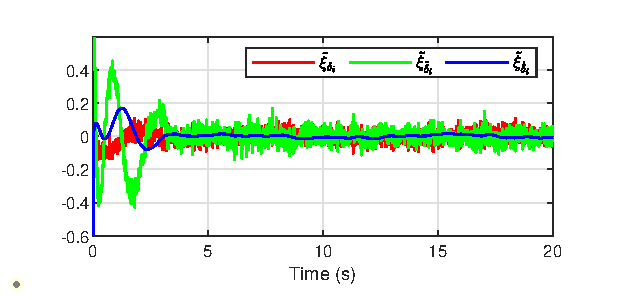
\includegraphics[scale=0.9]{ch3/img/matlab_error_case_2.eps}
    \caption{State estimation case 1.}%under the attack~\eqref{attack1}} 
    \label{fig:case1}
\end{figure}


\begin{figure}
    \centering
    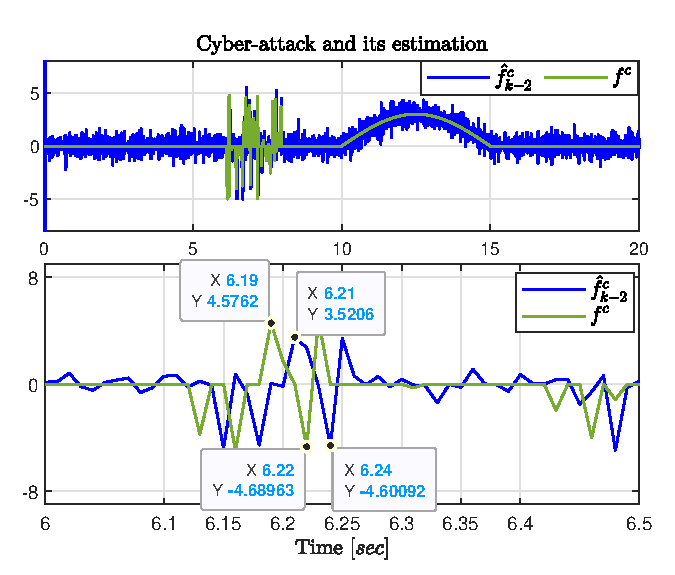
\includegraphics[scale=0.7]{ch3/img/matlab_fc_2.eps}
    \caption{Attack estimation using UIO case 1.}
    \label{fig:case1_fc}
\end{figure}


%  (since the plot of the results for this scenario
% is almost the same as Fig. 8, it is omitted to avoid repetition)
%{\color{blue}


For the second case of time-varying and bounded attack signal~\eqref{attack2}, it can be observed from the Figure~\ref{fig:case2_fc} that the cyberattack signal is accurately estimated, and the estimation error is bound.


\begin{figure}
    \centering
    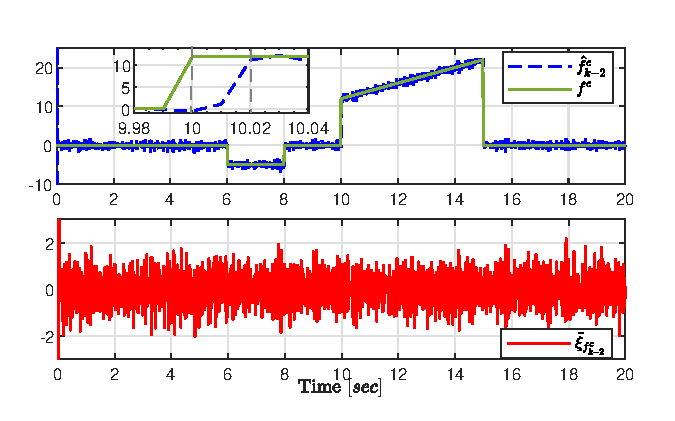
\includegraphics[scale=0.8]{ch3/img/matlab_fc_1.eps}
    \caption{Attack estimation and the errors case 2.}
    \label{fig:case2_fc}
\end{figure}

We can see that the proposed observer can estimate the the full state with good accuracy, while the unknown input is reconstructed with a fixed delay of two units based on the available output measurements. 

%}

%\begin{comment}
%
%\begin{figure}[h!]
%    \centering
%    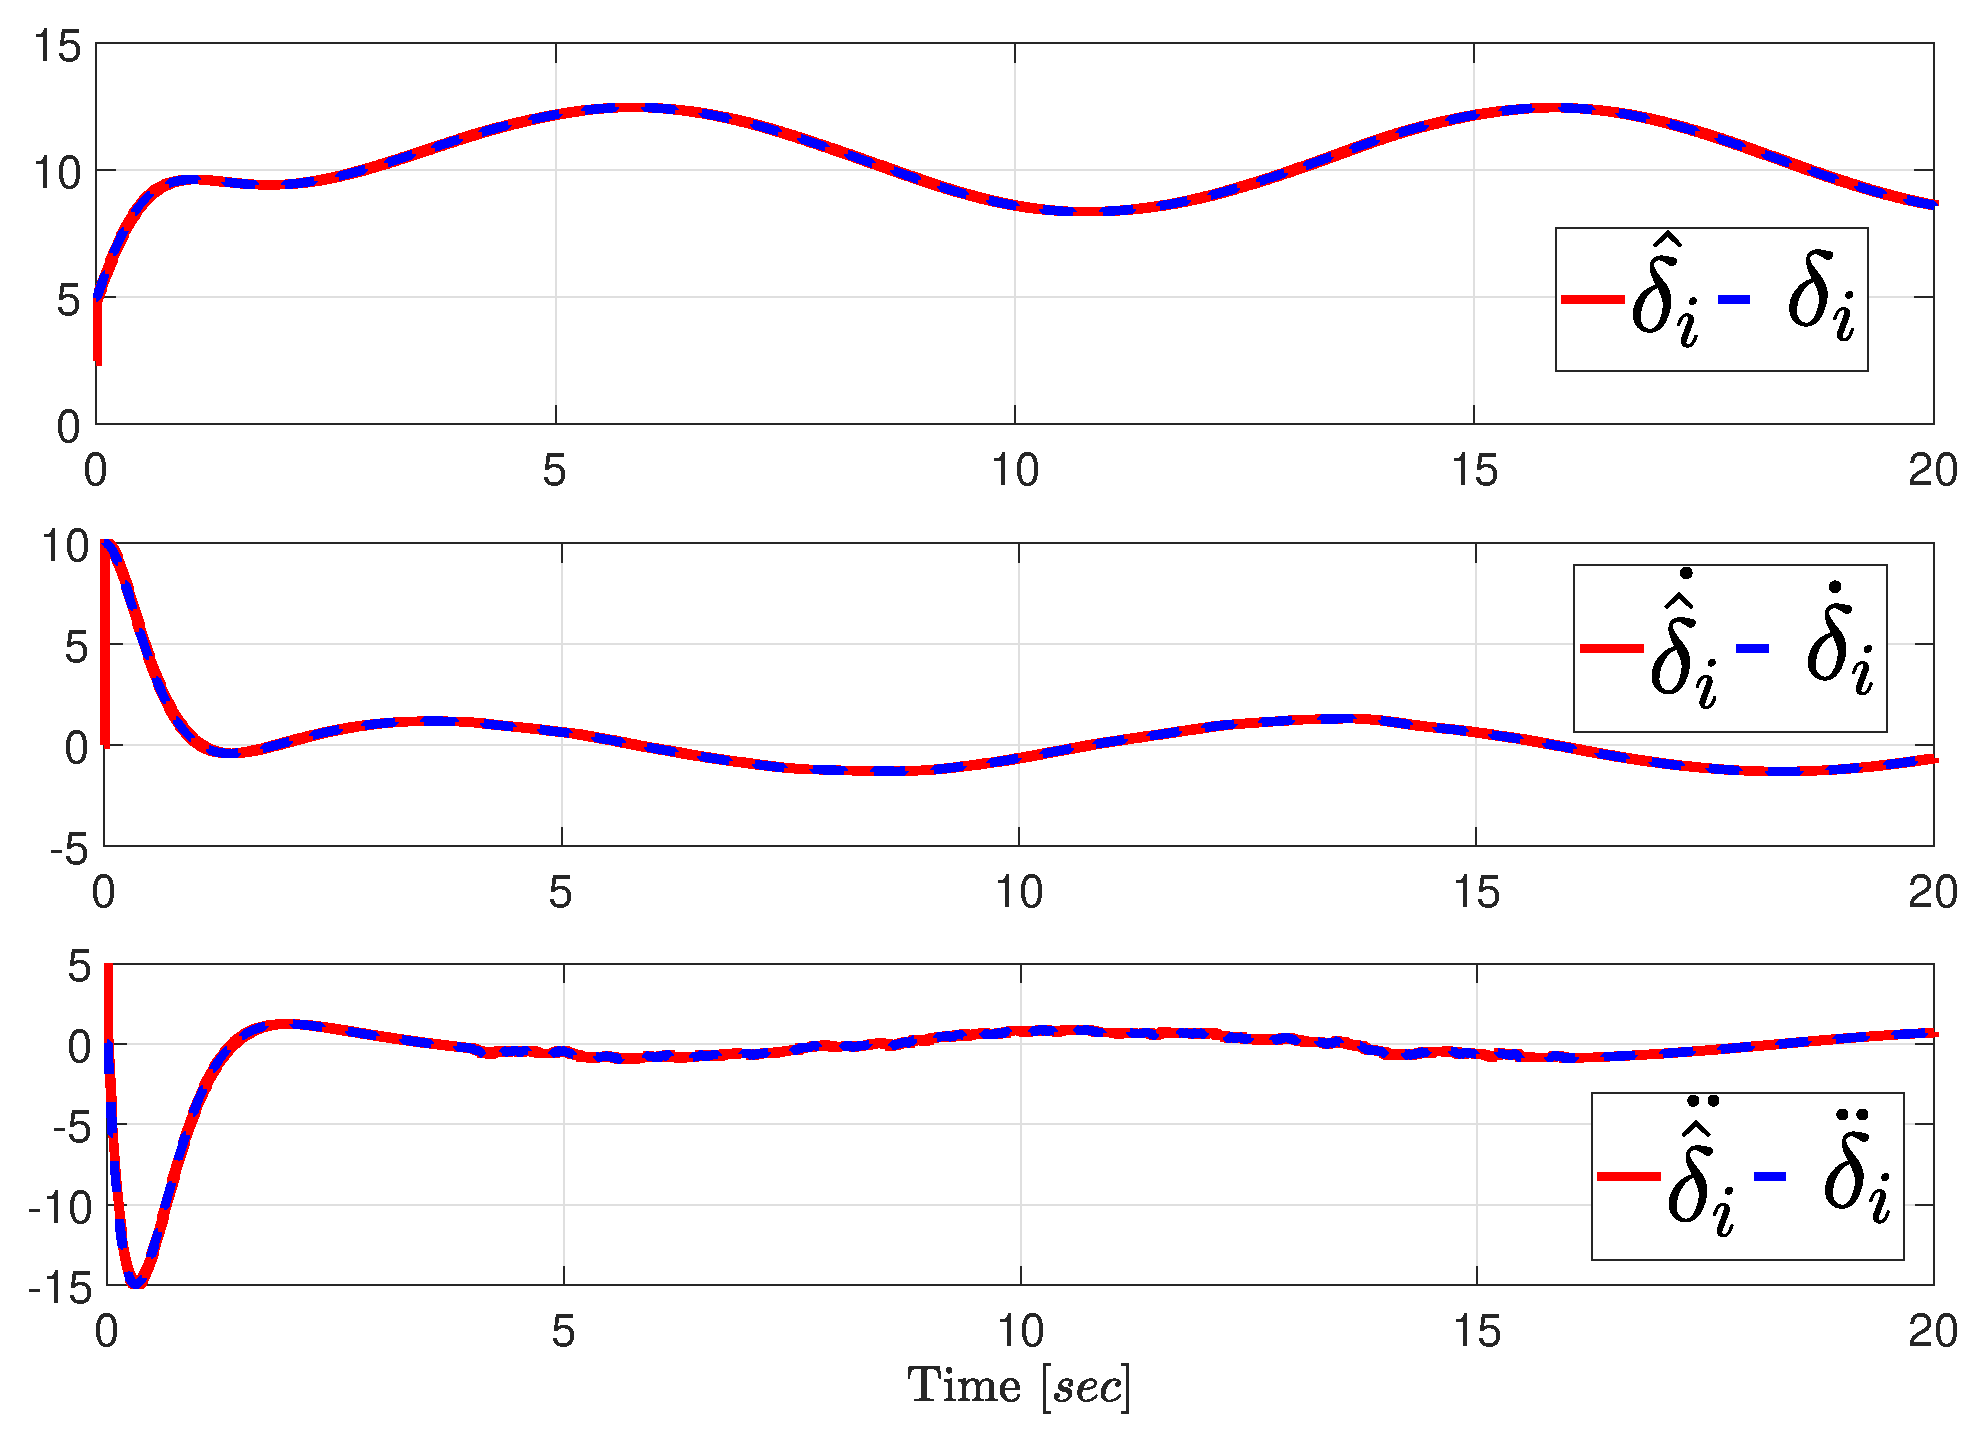
\includegraphics[width=0.4\textwidth, height=5cm]{img/case2.eps}
%    \caption{UIO state estimation case 2 }%under the attack~\eqref{attack2}}
%    \label{fig:case2}
%\end{figure}
%\begin{figure}
%    \centering
%    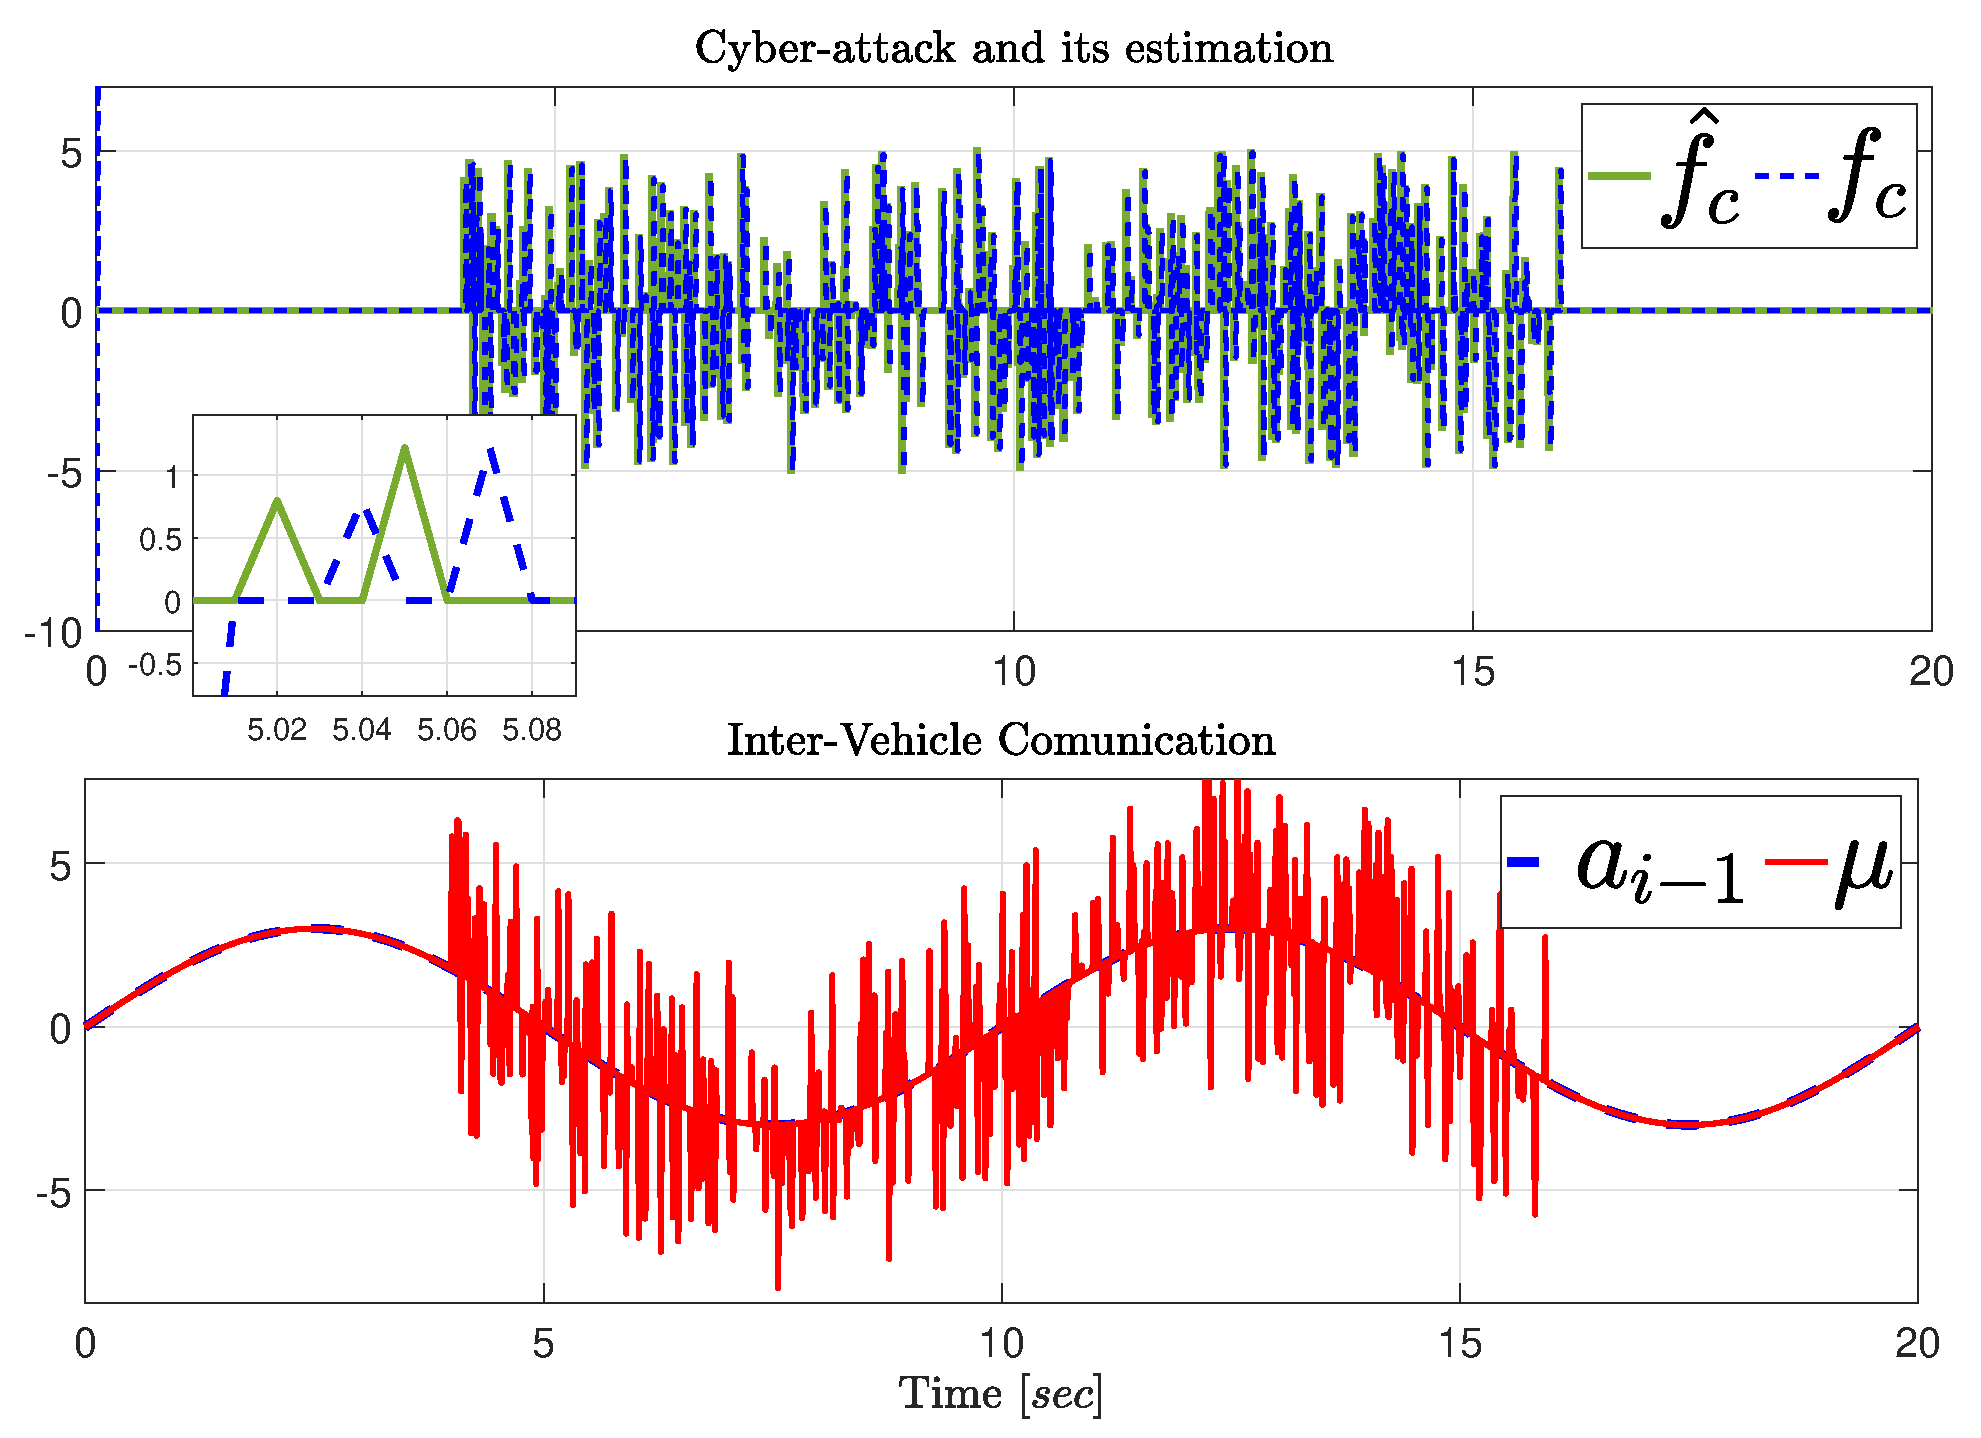
\includegraphics[width=0.4\textwidth,height = 5cm]{img/case2_fc.eps}
%    \caption{Attack estimation by UIO, case 2}
%    \label{fig:case2_fc}
%\end{figure}
%\end{comment}
%
%\begin{comment}
%    
%\pagebreak 
%\begin{remark}
%If the disturbance $\omega_{t}$ affects the second part of the state vector, $\dot{\delta}_i$, in either the system or measurement, it will impact the system's accuracy in estimating the attack $f^c$. Therefore, detecting attacks is only possible if the measurement of relative velocity remains untainted.
%\end{remark}
%
%\end{comment}

% \vspace*{-0.3cm}
\subsection{Simulation result using Carla}
%----
{
\color{black}

To evaluate the system under more realistic conditions, we conducted simulations within the CARLA simulator. Specifically, we simulated a scenario where a leading vehicle utilized a PID controller for cruise control, aiming to maintain a velocity of $10m/s$. We kept the parameters consistent with those listed in Table~\ref{tab:simple} and adopted a time step of $t_s = 0.04$. We also implemented a deterministic attack signal that varies over time and is defined by equation~\eqref{attack2}. As depicted in Fig~\ref{fig:carla_state}, the error state vectors for relative position and relative velocity exhibit good tracking, but the third vector $\tilde{\xi}_{a}$ falls short of perfection. This is because the acceleration of the preceding vehicle in Fig~\ref{fig:carla_fc} sent to the network is inconsistent, which affects the attack estimation performance. Fig~\ref{fig:carla_fc} illustrates the observer taking at least 5 seconds to converge to the actual state, and the estimated value being influenced by noise and imperfection of the model. However, the leading vehicle retains its ability to detect the cyberattack signal, ensuring a safe distance effectively}. A video showcasing the simulation scenario is provided in~\href{https://github.com/kslhuy/CACC_UIO_simulink}{GitHub repository}. Fig.~\ref{fig:carla_img} displays a thumbnail from the video.
 %~\cite{CarlaSimulator}
 \begin{figure}[h!]
     \centering    
     \includegraphics[width=0.4\textwidth,height = 3.5cm]{ch3/img/carla_d.png}
    \caption{Carla Simulator platform~(\href{https://github.com/kslhuy/CACC_UIO_simulink}{GitHub repository}).}
     \label{fig:carla_img}
 \end{figure}

\begin{figure}[h!]
    \centering    
    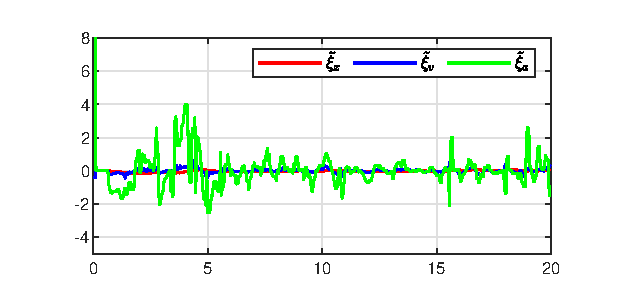
\includegraphics[scale=0.9]{ch3/img/state_carla_new.eps}
    \caption{State estimation using CARLA under attack case 2.}
    \label{fig:carla_state}
\end{figure}
\begin{figure}[h!]
    \centering    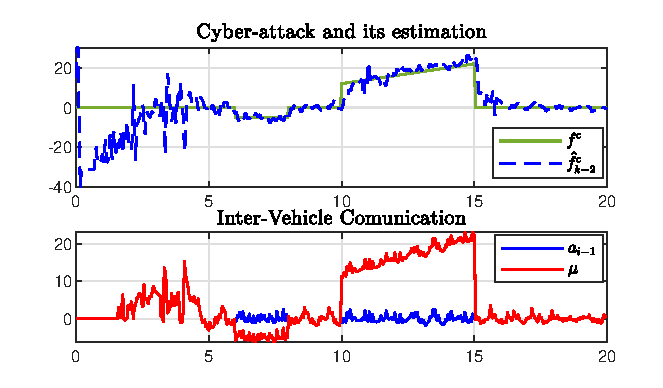
\includegraphics[scale=0.8]{ch3/img/fc_carla_new.eps}
    \caption{Cyberattack signal and inter-vehicle communication case 2.}
    \label{fig:carla_fc}
\end{figure}
%[GitHub repository](https://github.com/kslhuy/CACC_UIO_simulink).

% \pagebreak 











%======
\section{Exact Discretization Approach}\label{sec_Exact discretization}
%---

The observer design developed in the previous sections relies on a discrete-time model obtained via Euler discretization. This choice is deliberate, as it preserves the structure of the continuous-time system and allows direct application of well-established UIO existence and stability theorems. However, this discretization introduces a structural limitation, namely the violation of the rank condition, which necessitates the use of delayed outputs. The delay introduced in the previous sections is a discretization artifact, not a physical requirement.
{\color{blue}
In this section, we show that the delay requirement is not intrinsic to the continuous-time dynamics of the CACC system, but rather induced by the Euler discretization method. Physically, an input force affects acceleration instantly, which in turn influences velocity and position over any time interval $\Delta t$. 
The Euler method ($p_{k+1} = p_k + \Delta t \cdot v_k$) effectively ignores the direct influence of acceleration on position within the sampling step, severing the algebraic link required for the rank condition. 
By adopting an exact discretization based on the matrix exponential~\cite{M.Zhang}, the discrete-time model captures the complete evolution of the state trajectories between samples. This integration naturally couples the input with the position and velocity states through the matrix exponential, effectively preserving higher-order dynamics (such as $\frac{1}{2} a \Delta t^2$). This restores the structural coupling between the unknown input and the measured output, allowing the construction of a delay-free UIO. This approach offers significant advantages, including improved responsiveness and a simplified observer structure.
}
Figure~\ref{fig_dis_UIO} illustrates the structure of the proposed observer-based cyberattack estimation framework using the exact discretization model.

\begin{figure}[h!]
\centering
\includegraphics[width=7cm]{ch3/img/probleme_2.png}
\caption{Discrete-time model-based UIO}
\label{fig_dis_UIO}
\end{figure}



Following the exact discretization method detailed in~\cite{M.Zhang}, the discrete-time model of the CACC system is given by:
\begin{equation}\label{CACC_discrete_2}
      \left\{ \begin{array}{l}
        x_{k+1} = A_d x_{k} + B_d v_{i,k} +F_d  \mu_{k}+ \hat{\Delta} - W_d  f^c_{k} \\
            y_{k} = C_d x_{k}\end{array}\right.
\end{equation}  
where the system matrices are computed as:
\begin{align*}
    A_d &= e^{A T_s}, \quad B_d =\int_{0}^{T_s} e^{A \eta} B d\eta, \quad C_d = C, \\
    F_d &= \int_{0}^{T_s} e^{A \eta} F d\eta, \quad W_d = \int_{0}^{T_s} e^{A \eta} W d\eta, \quad \hat{\Delta} = \int_{0}^{T_s} e^{A \eta} \Delta d\eta,
\end{align*}
with $T_s$ denoting the sampling period.

We now verify the rank condition for the discretized system~\eqref{CACC_discrete_2}. Using the system parameters given in Table~\ref{tab:simple}, we obtain:
\[
C_d W_d = \begin{pmatrix}
1 & 0 & 0 \\
0 & 1 & 0
\end{pmatrix} 
\begin{pmatrix}
1.14\times 10^{-6}\\
3.41\times 10^{-4}\\
6.75\times 10^{-2}
\end{pmatrix} 
= \begin{pmatrix}
    1.14\times 10^{-6}\\
    3.41\times 10^{-4}
\end{pmatrix} \neq 0.
\]
Since $C_d W_d \neq 0$, the rank condition $\rank(C_d W_d) = \rank(W_d) = 1$ is satisfied. This confirms that the unknown input $f^c_k$ can be estimated directly from the output $y_k$ without requiring any delay.






%============
\subsection{Simulation Results and Comparison}\label{sec4}
%--
To demonstrate the effectiveness of the exact discretization method and the proposed observer, we conducted simulations using MATLAB and CARLA, following the procedures outlined in~\cite{nguyen2020cyberattack}. This section presents the results obtained with our method and compares them with those from~\cite{nguyen2020cyberattack}.

We solve the LMI conditions for the observer gain using the YALMIP Toolbox with the exponential stability parameter $\alpha=0.5$. The resulting observer gain $K$ is:
\[
K = \begin{pmatrix}
0.5 & -0.005 \\
-0.001 & 0.7 \\
-0.2 & -68.0 \\
2.2 & 1004.2 
\end{pmatrix}
\]

\begin{figure}[h!]
    \centering 
    \includegraphics[scale=0.45]{ch3/img/error_state_mat.png}
    \caption{State estimation error using the proposed exact discretization method.}
    \label{est_error_sel_fig}
    
    \vspace{0.5cm}
    
    \centering 
    \includegraphics[scale=0.3]{ch3/img/erreur.png}
    \caption{State estimation error from~\cite{nguyen2020cyberattack}.}
    \label{est_error_sel_fig_huy}
\end{figure}

Figures~\ref{est_error_sel_fig} and~\ref{est_error_sel_fig_huy} illustrate the estimation errors for the system states (position, velocity, and acceleration). Figure~\ref{est_error_sel_fig_huy} shows the results from~\cite{nguyen2020cyberattack}, where the estimation errors exhibit significant initial oscillations lasting about 5 seconds before stabilizing. Furthermore, the noise amplitude is substantial, indicating reduced accuracy under cyberattacks.

In contrast, Figure~\ref{est_error_sel_fig} shows the results obtained with our exact discretization method. The initial oscillations are less pronounced, and the system stabilizes more rapidly (within approximately 3 seconds). Moreover, the noise amplitude in both position and velocity errors is significantly reduced. This demonstrates the superior accuracy and robustness of the proposed method. Notably, the velocity estimation error is much smaller compared to the method in~\cite{nguyen2020cyberattack}.

\begin{figure}[h!]
    \centering 
    \includegraphics[scale=0.4]{ch3/img/photo1.png}
    \caption{Cyberattack estimation and error using the proposed method.}
    \label{fig:attack_est}

    \vspace{0.5cm}

    \centering 
    \includegraphics[scale=0.4]{ch3/img/cyberattack.png}
    \caption{Cyberattack estimation and error from~\cite{nguyen2020cyberattack}.}
    \label{fig:attack_est_huy}
\end{figure}

Figures~\ref{fig:attack_est} and~\ref{fig:attack_est_huy} depict the actual cyberattack signal (blue) and its estimate (green), along with the estimation error. Both methods detect the attack, but our method (Figure~\ref{fig:attack_est}) exhibits superior performance. The estimated signal shows fewer fluctuations and greater stability compared to~\cite{nguyen2020cyberattack} (Figure~\ref{fig:attack_est_huy}).

The estimation error in our method is centered around zero with minimal fluctuations (amplitude $\approx 0.6$), whereas the method from~\cite{nguyen2020cyberattack} shows errors with an amplitude of around 2. This higher noise level in the previous method could compromise reliability in safety-critical scenarios.

\subsubsection{CARLA Simulator Results}
To validate the proposed method under more realistic conditions, we conducted tests using the CARLA simulator. We implemented the same scenario as in~\cite{nguyen2020cyberattack}, involving a lead vehicle and a following vehicle. The lead vehicle maintains a reference speed of 10 m/s using a PID controller. The simulation parameters match those used in the MATLAB simulation, with a time step of 0.04 seconds.

\begin{figure}[h!]
    \centering 
    \includegraphics[scale=0.32]{ch3/img/err_moi.png}
    \caption{State estimation error in CARLA using the proposed method.}
    \label{fig:carla_error_moi}
    
    \vspace{0.5cm}
    
    \centering 
    \includegraphics[scale=0.45]{ch3/img/carla erreur.png}
    \caption{State estimation error in CARLA from~\cite{nguyen2020cyberattack}.}
    \label{fig:carla_error_huy}
\end{figure}

Figures~\ref{fig:carla_error_moi} and~\ref{fig:carla_error_huy} compare the state estimation errors in the CARLA environment. With our method (Figure~\ref{fig:carla_error_moi}), the position and velocity errors converge to zero more rapidly than in~\cite{nguyen2020cyberattack} (Figure~\ref{fig:carla_error_huy}). The acceleration estimation takes about 5 seconds to stabilize, which is comparable to the reference method.

\begin{figure}[h!]
    \centering 
    \includegraphics[scale=0.52]{ch3/img/fc_moi.png}
    \caption{Cyberattack estimation in CARLA using the proposed method.}
    \label{fig:carla_attack_moi}
    
    \vspace{0.5cm}
    
    \centering 
    \includegraphics[scale=0.47]{ch3/img/fc_huy.png}
    \caption{Cyberattack estimation in CARLA from~\cite{nguyen2020cyberattack}.}
    \label{fig:carla_attack_huy}
\end{figure}

Figures~\ref{fig:carla_attack_moi} and~\ref{fig:carla_attack_huy} present the cyberattack estimation results. Our method (Figure~\ref{fig:carla_attack_moi}) demonstrates better initial error management with smaller fluctuations compared to the significant transient instability observed in~\cite{nguyen2020cyberattack} (Figure~\ref{fig:carla_attack_huy}).

Furthermore, our method achieves faster convergence, accurately estimating the cyberattack within 3 seconds, whereas the reference method requires more than 5 seconds. In terms of long-term accuracy, our method tracks the actual cyberattack signal $f^c$ more closely, providing a more precise estimation than the method in~\cite{nguyen2020cyberattack}.

\section{Conclusion}
This chapter addressed the problem of resilient state estimation and cyberattack reconstruction for Connected Autonomous Vehicles (CAVs) operating in a Cooperative Adaptive Cruise Control (CACC) platoon. The primary challenge identified was the violation of the rank condition required for standard Unknown Input Observer (UIO) design when using classical Euler discretization.

To overcome this, we first proposed a discrete-time UIO design based on output delay. By shifting the output measurement backward, we recovered the necessary algebraic coupling between the unknown input and the measured output, enabling the simultaneous estimation of vehicle states and attack signals. We derived Linear Matrix Inequality (LMI) conditions to guarantee the Input-to-State Stability (ISS) of the estimation error in the presence of bounded disturbances.

Subsequently, we introduced a refined approach using exact discretization based on the matrix exponential. We demonstrated that the rank condition failure was an artifact of the Euler approximation rather than an intrinsic system limitation. The exact discretization method naturally preserves the higher-order dynamics, restoring the rank condition without the need for artificial delays.

Comparative simulations in both MATLAB and the high-fidelity CARLA simulator validated the effectiveness of both approaches. The results confirmed that while the delayed-output method is effective, the exact discretization approach offers superior performance in terms of convergence speed, estimation accuracy, and robustness to noise.

Future work will focus on extending these resilient estimation strategies to multi-vehicle platoons with heterogeneous dynamics and investigating the impact of model parameter uncertainties. Additionally, we aim to integrate this observer-based detection with active fault-tolerant control strategies to further enhance the safety and resilience of autonomous transportation systems.
% \section{Conclusion}


\chapter[Titre court du 2nd chapitre pour sommaire]{Le titre long du second chapitre du manuscrit de thèse}\label{chp2_chap}
\chaptermark{Titre chp 2 pour en tete de page}

\objectif{Objectif rapide du chapitre 2.}

%%%%%%%%%%%%%%%%%%%%%%%%%%%%%%%%%%%%%%%%%%%%%%%%%%%%%%%%%%%%%%%%%%%%%%%%%%%%%%%%%%%%%%%%%%%%%%%%%
\section{Introduction}
%%%%%%%%%%%%%%%%%%%%%%%%%%%%%%%%%%%%%%%%%%%%%%%%%%%%%%%%%%%%%%%%%%%%%%%%%%%%%%%%%%%%%%%%%%%%%%%%%
\section{Problem Formulation and Motivation}\label{sec2}
%
In this paper, we consider the class of continuous-time nonlinear systems in state-space form described by the following equations:

\begin{equation}\label{sys_1}
    \begin{array}{l}
        \dot{x} = \varphi(x,u) + B\mu_{x}  \\
        y = Cx, 
    \end{array}
\end{equation}
where $x\in \mathcal{X} \subseteq\mathbb{R}^{n_x}$ is the state vector, $y\in\mathbb{R}^{n_y}$ is the output measurement, $u\in\mathcal{U} \subseteq\mathbb{R}^{n_u}$ is the control input, and $\mu_{x}\in\mathbb{R}^{n_{\mu}}$ is an unknown nonlinear function that encapsulates the system uncertainty including both unmodeled dynamics and external disturbances. The matrices $C\in\mathbb{R}^{n_y}\times\mathbb{R}^{n_x}$ and $B\in\mathbb{R}^{n_x}\times\mathbb{R}^{n_{\mu}}$ are constant and known matrices. The function $\varphi: \mathcal{X} \times \mathcal{U} \to \mathbb{R}^{n_x}$ represents the known nonlinear component of the system. 

\begin{remark}
For simplicity, we consider systems with linear output. Otherwise, if we have nonlinear output $y = h(x)$, we introduce a new state $\eta(t)$, with $\dot{\eta} \triangleq A_{\eta} \eta + \gamma y$ and $\eta_0 = \eta(0)$ known. Then, a new system with the augmented vector $\zeta = \begin{bmatrix} \eta \\ x \end{bmatrix}$ may be considered, which has as linear output the vector $\eta$.
\end{remark}


Now, let us introduce the following assumptions which are required for our unknown input observer design methods.
\begin{assumption}\label{ali_hyp1}
%Assumption 1. 
The output vector $y$ has dimension greater than or equal to the number of unknown terms~$\mu_{x}$; equivalently, $n_{\mu} \leq n_y$.
\end{assumption}

\begin{assumption}\label{ali_hyp2}
%Assumption 2. 
The nonlinear function $\varphi(.)$ is $\gamma_{\varphi}-$Lipschitz continuous on $\mathcal{X}$, uniformly on $u\in\mathcal{U}$.
\end{assumption}

\begin{assumption}\label{ali_hyp3}
The unknown nonlinearity $\mu_{x}(.)$ is Lebesgue measurable and $\mathcal{L}_{2}-$bounded.
\end{assumption}

The objective of this paper is to estimate the unmodeled dynamics $\mu_{x}$. More specifically, we propose to estimate $\mu_{x}$ by combining an unknown input observer~(UIO) with a neural network--based approach, leveraging gradient-based methods to better capture the unmodeled components of the system. The key idea is to incorporate the UIO-based estimation into the loss function of the neural network, thereby enhancing residual regularization and ensuring consistency with the UIO. This, in turn, improves the robustness and performance of the overall estimation scheme. Unfortunately, it is not possible to estimate the unknown input, $\mu_x$, if the system fails to satisfy the following main necessary condition:
\begin{equation}\label{rank}
\textrm{rank}(C B) = \textrm{rank}(B).
\end{equation}
%
In addition, to be able to directly construct a UIO for system~\eqref{sys_1} to estimate simultaneously $x$ and $\mu_x$, the constraint~\eqref{rank} is not sufficient. For this, we should be able to write the system under the form:
\begin{equation}\label{sys_2}
    \begin{array}{l}
        \mathbb{E} \dot{\zeta} = \varphi_{\zeta}(\zeta,u)  \\
        y = \mathcal{H} \zeta
    \end{array}
\end{equation}
with
\begin{equation}\label{rank2}
\textrm{rank}\left( \begin{bmatrix} \mathbb{E} \\  \mathcal{H} \end{bmatrix} \right) = n_{x} + n_{\mu}.
\end{equation}
%--
For further details on this requirement, the reader is referred to~\cite{chaouche2022unknown,trinh2011functional,Zemouche-Boutayeb-2009,Hassan13a,Trinh:TAC08} and the references therein. 

% % %%% Simple details of problem

% Various techniques address the rank condition issue. Some invert system dynamics [13]–[15] or rely on output derivatives [13], [16], which amplifies noise. Others augment the system with additional sensors [13], which increases cost. Proportional-Integral Observers (PIO) often assume null dynamics [17], [18] or constant inputs [19], which is overly conservative for vehicle dynamics. 
% % %%% Simple details of problem


%%% TOO much details of the literature
To address this challenge, various techniques have been proposed in the literature, each offering a different approach to the problem. Without aiming for exhaustiveness, these techniques can be summarized as follows. Nevertheless, the problem remains open, and new ideas or improvements are still possible, although often at the cost of additional assumptions:
%==
\begin{itemize}
\item {\it Inverting the system dynamics:} The system state is first estimated, and the unknown inputs are then obtained by inverting the dynamics~\cite{Phanomchoeng:ASME/TM14,Benallouch:TCST17,Marquez:Auto14}. However, the presence of disturbances and nonlinearities in the output signal or in the dynamics can make the problem particularly challenging.
%



\item {\it Deriving the output vector $y(t)$:} In some cases, the derivatives of the output measurements are required~\cite{Hou:256351,Phanomchoeng:ASME/TM14}. This leads to the construction of a pseudo-output vector $y_{\rm new}$, which enables the simultaneous estimation of $x$ and $\mu_{x}$. For instance, in the linear case without disturbances, one obtains 
$$
y_{\rm new} = C_{\rm new} x + C_{\mu}\mu_{x},
$$
where $\mathrm{rank}(C_{\mu}) = n_{\mu}$. However, this approach is not suitable for nonlinear disturbed systems, since differentiating $y(t)$ introduces additional variables arising from the derivatives of the disturbance vector, as well as new nonlinearities in the pseudo-output vector. Consequently, satisfying the rank condition~\eqref{rank} with the new matrices becomes very difficult.

%
\item {\it Adding sensors:} In some cases, augmenting the system with additional sensors is a natural way to overcome the rank condition~\eqref{rank}. This approach introduces a new measurement vector $y_{\rm new}$, where the original output $y(t)$ is used to estimate the state $x(t)$, and the additional outputs $y_{\rm new}$ are exploited to estimate the unknown input, $\mu_{x}$. For example, in~\cite{Phanomchoeng:ASME/TM14} (and references therein), four sensors (i.e., four output measurements) were employed to estimate only two unknown inputs. However, the presence of disturbances can significantly decrease estimation performance. Moreover, additional sensors may be very expensive or, in some cases, unavailable.
%
\item {\it Proportional--Integral Observer and Null Dynamics:} Some works in the literature have employed a Proportional--Integral Observer (PIO) together with null dynamics imposed on the estimated unknown input~\cite{PIO_1995,PIOreview}. However, this assumption does not reflect the true dynamics of the unknown input, leading to inaccurate estimation. Other approaches assume constant inputs~\cite{jeon2020simultaneous}, i.e., $\dot{\mu}_{x} \equiv 0$, but this restriction is overly conservative. Recently, a method for discrete-time systems was proposed in~\cite{nguyen2024cyberattack}; however, this approach yields delayed estimates of both the system state and the unknown inputs, which is often impractical to design reliable controllers.
\end{itemize}
%%%%

The limitations of the aforementioned methods motivated us to adopt a different approach and propose a simple strategy to estimate the system state and the unknown input without relying on conservative assumptions. The key idea is to recognize that this initial estimation is not final. Rather, the objective is to provide a first-level approximation of $x$ and $\mu_{x}$, which will subsequently be refined through the neuro-adaptive observer we introduce later. This refinement enhances estimation accuracy and ultimately yields a definitive estimate of the unmodeled nonlinearity, $\mu_{x}$.


The strategy consists in rewriting system~\eqref{sys_1} without modifying it. Then, the UIO we will propose will be based on reliable approximation of~\eqref{sys_1}.

\begin{equation}\label{ali_syst1}
    \begin{array}{l}
        \dot{x} + E_{\delta_1} \dot{\mu}_{x} = \varphi(x,u) + B\mu_{x} + E \omega_{\delta_{1}} \\
        y = Cx + D_{\delta_2} \mu_{x} + D\, \omega_{\delta_{2}} 
    \end{array}
\end{equation}
where $D \in \mathbb{R}^{n_y \times n_{\mu}}$ and $E \in \mathbb{R}^{n_x \times n_{\mu}}$ are given constant, full-column-rank matrix specified by the user; $E_{\delta_1} = \delta_{1} E, D_{\delta_2} = \delta_{2} D$; and $\omega_{\delta_{1}}(t) = \delta_{1} \dot{\mu}_{x}(t), \omega_{\delta_{2}}(t) = \delta_{2} \mu_{x}(t)$, with $\delta_{j} \geq 0$, with $(\delta_1,\delta_2) \neq (0,0)$, chosen sufficiently small to ensure the feasibility of some sufficient conditions that will be stated later. The purpose of this reformulation is to recover the rank condition~\eqref{rank2}, at the expense of introducing the additive terms $\omega_{\delta_{j}}(t), j=1,2$, which are handled as disturbances. 

The next section presents LMI conditions that guarantee accurate estimation of $x$ and $\mu_{x}$ while satisfying an $\mathcal{H}_{\infty}$ criterion, or more specifically, an $\mathcal{L}_{2}$-optimality criterion---where the performance bound is proportional to $\delta_{j}, j=1,2$.








\section{LMI-Based $\mathcal{H}^{1}$ UIO Design}\label{uio}
%==  $\mathcal{W}^{1,2}$
This section is devoted to the numerical LMI-based design procedure ensuring the asymptotic estimation of the system state $x$ and the unmodeled dynamics $\mu_{x}$ following a $\mathcal{H}^{1}-$optimality criterion.

%===========
\subsection{System transformation}
%-----
Recall that $\mathcal{H}^{1}$ is the {\it Hilbert} space corresponding to the {\it Sobolev} space, $\mathcal{W}^{1,2}$, of square--integrable functions whose weak first derivatives are also square--integrable. Mathematically, we define the set $\mathcal{H}^{1}\left( \Omega \right)$ as
$$
\mathcal{H}^{1}\left( \Omega \right) := \left\{ \psi \in \mathcal{L}^{2}(\Omega) \;\middle|\; \frac{\textrm{d} \psi}{\textrm{d} t} \in \mathcal{L}^{2}(\Omega) \right\}
$$
with $\Omega = [0~+\infty[$ in our case. This space is endowed by the norm $\| . \|_{\mathcal{H}^{1}}$ defined as follows:
$$
\| \psi \|_{\mathcal{H}^{1}} :=
\left( \| \psi \|_{\mathcal{L}^{2}}^2 + \left\| \frac{\textrm{d} \psi}{\textrm{d} t} \right\|_{\mathcal{L}^{2}}^2 \right)^{1/2}.
$$

First, system~\eqref{ali_syst1} can be rewritten under the compact form:
\begin{equation}\label{ali_syst2}
    \begin{array}{l}
        \mathbb{E} \dot{\zeta} = \varphi_{\zeta}(\zeta,u) + \bar{E} \bm{\omega}_{\delta} \\
        y = \mathcal{H} \zeta + \bar{D} \bm{\omega}_{\delta}
    \end{array}
\end{equation}
where
\begin{subequations}\label{ali_syst2_e1}
\begin{equation}\label{ali_syst2_e1_1}
\mathbb{E} := \begin{bmatrix} \mathbb{I}_{n_x} & E_{\delta_1} \end{bmatrix},~\mathcal{H} := \begin{bmatrix} C & D_{\delta_2} \end{bmatrix},
\end{equation}
%
\begin{equation}\label{ali_syst2_e1_2}
\bar{E} := \begin{bmatrix} E & 0_{n_{x}\times n_{\mu}} \end{bmatrix},~\bar{D} := \begin{bmatrix} 0_{n_{y}\times n_{\mu}} & D \end{bmatrix},
\end{equation}
%
\begin{align}\label{ali_syst2_e1_3}
\zeta := \begin{bmatrix} x \\ \mu_{x} \end{bmatrix},~\bm{\omega}_{\delta} := \begin{bmatrix} \omega_{\delta_{1}} \\ \omega_{\delta_{2}} \end{bmatrix},
\end{align}
%
%\vspace{-0.7cm}
\begin{align}\label{ali_syst2_e1_4}
\varphi_{\zeta}(\zeta,u) := \varphi(x,u) + B \mu_{x}.
\end{align}
\end{subequations}
%==
%
Now, let us introduce the following necessary assumption:
\begin{assumption}\label{ali_hyp4}
The matrices $E$ and $D$ are chosen such that $\mathbb{E}$ and $\mathcal{H}$ satisfy the rank condition~\eqref{rank2}.
\end{assumption}

The objective is to design a state observer that provides an estimate $\hat{\zeta}$ of $\zeta$, such that the following $\mathcal{H}^1$-optimality inequality holds:
%
\begin{align}%\label{ali_h1_e1}
\| \tilde{\zeta} \|_{\mathcal{H}^{1}} &\leq \lambda_{\delta} \, \left\| \mu_{x} \right\|_{\mathcal{H}^{1}}  + \beta \, \left\| \xi_0 \right\| \label{ali_h1_e1_2}
\end{align}
where $\tilde{\zeta} := \zeta - \hat{\zeta}$, $\lambda_{\delta}$ is the disturbance attenuation level, explicitly depending on $\delta_1$ and $\delta_2$, $\beta > 0$ is a weighting real constant, and $\xi_0$ is a vector depending on $\tilde{\zeta}(0)$ and $\mu_{x}(0)$.%$\mathcal{N}\left(\tilde{\zeta}(0), \mu_{x}(0)\right)$. $\xi_0 := \tilde{\zeta}(0) - D \mu_{x}(0)$
%--
%===========
\subsection{UIO structure and error dynamics}
%-----
From Assumption~\ref{ali_hyp4},  there exist two matrices $P_{\zeta}$ and $Q_{\zeta}$ such that
\begin{equation}\label{ali_syst2_e2}
 P_{\zeta} \mathbb{E} + Q_{\zeta} \mathcal{H} = \mathbb{I}_{n_{\zeta}}.
\end{equation}
where $n_{\zeta} := n_{x} + n_{\mu}$. These matrices are exploited in the following observer structure:
\begin{equation}\label{ali_syst2_e3}
\left\{
\begin{array}{rcl}
\dot{\eta} & = & P_{\zeta} \varphi_{\zeta}(\hat{\zeta},u) + K \left( y - \mathcal{H} \hat{\zeta} \right)
\\
\hat{\zeta} & = & \eta + Q_{\zeta} y 
\end{array}
\right.
\end{equation}
where $\hat{\zeta}$ is the estimate of $\zeta$ and $K \in\mathbb{R}^{n_{\zeta}}\times\mathbb{R}^{n_y}$ is the observer gain to be determined such that the estimation error, $\tilde{\zeta} : = \zeta - \hat{\zeta}$, satisfies the $\mathcal{H}^1$-optimality criterion~\eqref{ali_h1_e1_2} with appropriate $\lambda_{\delta}, \beta$, and $\xi_0$.
%

We have 

\begin{align}\label{ali_syst2_e4}
\tilde{\zeta} &= \zeta - \eta - Q_{\zeta} y \notag \\
&= \left(\mathbb{I}_{n_{\zeta}} - Q_{\zeta} \mathcal{H}\right) \zeta - \eta - Q_{\zeta} \bar{D} \bm{\omega}_{\delta} \notag \\
&\overbrace{ \mathrel{\scalebox{2}[1]{=}} }^{\eqref{ali_syst2_e2}} P_{\zeta} \mathbb{E} \zeta - \eta - Q_{\zeta} \bar{D} \bm{\omega}_{\delta}
\end{align}
which gives equivalently
\begin{equation}\label{ali_syst2_e5}
\overbrace{ \tilde{\zeta} + Q_{\zeta} \bar{D} \bm{\omega}_{\delta} }^{\xi(t)} = P_{\zeta} \mathbb{E} \zeta(t) - \eta(t).
\end{equation}
It is worth noting that the reformulation~\eqref{ali_syst2_e5} conveniently avoids the derivative of $\bm{\omega}_{\delta}$ in the derivation of the error dynamics.

By using the dynamics~\eqref{ali_syst2} and~\eqref{ali_syst2_e3}, we obtain
\begin{align}\label{ali_syst2_e6}
\dot{\xi} &= P_{\zeta} \left[ \varphi_{\zeta}(\zeta,u) - \varphi_{\zeta}(\hat{\zeta},u) \right] -K \mathcal{H} \tilde{\zeta} \notag \\
&\quad + \left(P_{\zeta} \bar{E} - K \bar{D} \right) \bm{\omega}_{\delta} \notag \\
&= \left(P_{\zeta} \nabla^{\varphi_{\zeta}}_{\zeta}(\bm{z},u) - K  \mathcal{H} \right) \xi \notag \\
&\quad+ \Big( \mathcal{E}\left( \bm{z},u\right) - K  \mathcal{D} \Big) \bm{\omega}_{\delta}
\end{align}
where
$$
\mathcal{E}\left( \bm{z},u\right) := \bar{E} - P_{\zeta} \nabla^{\varphi_{\zeta}}_{\zeta}(\bm{z},u) Q_{\zeta} \bar{D}
$$
%==
$$
\mathcal{D} := \left( \mathbb{I}_{n_y} + \mathcal{H} Q_{\zeta} \right) \bar{D}.
$$
and from the differential mean value theorem~\cite{Hasni_LCSS_24}, we have
$$
\varphi_{\zeta}\left(\zeta,u \right) - \varphi_{\zeta}\left(\hat{\zeta},u \right) = \nabla^{\varphi_{\zeta}}_{\zeta}(\bm{z},u) \tilde{\zeta}
$$
for a given $\bm{z}$.

From this point onward, the analysis will be carried out with the vector~$\xi$ instead of~$\tilde{\zeta}$, and we will return to~$\tilde{\zeta}$ at the end to derive the final $\mathcal{H}^{1}$ bound~\eqref{ali_h1_e1_2}.
%===========
\subsection{New LMI-based UIO design conditions}
%-----
Before presenting the proposed LMI-based UIO design procedure, we state an intermediate and general result in the following proposition.
%-
\begin{proposition}\label{ali_prop1}
Le $\vartheta(.)$ be a Lyapunov function such that there exists $\vartheta_{\max} >0$ such that $\vartheta(z) \leq \vartheta_{\max}\| z \|^{2}$, for all $z \in \mathbb{R}^{n_\zeta}$. Consider a matrix $\mathcal{S} = \mathcal{S}^{\top} > 0$ and a real constant $\lambda >0$ such that the following inequality holds:
\begin{multline}\label{ali_prop1_e1}
\dot{\vartheta}(z) + \| z \|^{2} + \dot{z}^{\top} \mathcal{S} \dot{z} - \lambda \| w \|^{2} \leq 0,\\ 
\forall z \in \mathbb{R}^{n_\zeta}, w \in \mathbb{R}^{2n_{\mu}}
\end{multline}
%
with $z \in \mathcal{H}^{1}$ and $w \in \mathcal{L}^{2}$. Then, the following inequality is satisfied:
\begin{multline}\label{ali_prop1_e2}
\| z \|_{\mathcal{H}^{1}} \leq \sqrt{\frac{\lambda}{\min\left(1,\lambda_{\min}(\mathcal{S})\right)}} \| w \|_{\mathcal{L}^{2}}  \\
+\sqrt{\frac{\vartheta_{\max}}{\min\left(1,\lambda_{\min}(\mathcal{S})\right)}} \| z_0 \|.
\end{multline}
Moreover, if~\eqref{ali_prop1_e1} is satisfied with $z := \xi$ and $w := \bm{\omega}_{\delta}$, where $\xi$ and $\bm{\omega}_{\delta}$ are defined by~\eqref{ali_syst2_e5} and~\eqref{ali_syst2_e1_3}, respectively, then the estimation error, $\tilde{\zeta}$, satisfies the $\mathcal{H}^{1}$ bound~\eqref{ali_h1_e1_2} with $\lambda_{\delta}$, $\beta$, and $\xi_0$ given as follows:
\begin{subequations}
\begin{multline}\label{ali_prop1_e3}
\lambda_{\delta} := \delta_{2} \sigma_{\max}\left(Q_{\zeta} D\right) \\
+ \max\left(\delta_{1}, \delta_{2} \right) \sqrt{\frac{\lambda}{\min\left(1,\lambda_{\min}(\mathcal{S})\right)}}
\end{multline}
%--
\begin{equation}\label{ali_prop1_e4}
\beta := \sqrt{\frac{\vartheta_{\max}}{\min\left(1,\lambda_{\min}(\mathcal{S})\right)}}
\end{equation}
%--
\begin{equation}\label{ali_prop1_e5}
\xi_0 := \tilde{\zeta}(0) + Q_{\zeta} D \mu_{x}(0).
\end{equation}
\end{subequations}
where $\sigma_{\max}\left(Q_{\zeta} D\right)$ represents the largest singular value of the matrix $Q_{\zeta} D$.
\end{proposition}
%==
\begin{proof}
The first part of the proof is relatively straightforward. Before integrating~\eqref{ali_prop1_e1} to get the norms $\| . \|_{\mathcal{H}^{1}}$ and $\| . \|_{\mathcal{L}^{2}}$, take in mind that
$$
\min\left(1,\lambda_{\min}(\mathcal{S})\right) \left(  \| z \|^{2} +  \| \dot{z} \|^{2}  \right) \leq \| z \|^{2} + \dot{z}^{\top} \mathcal{S} \dot{z}.
$$
%
Hence, since 
$$
\int_{0}^{+\infty} \!\left( \| z(s) \|^{2} + \| \dot{z}(s) \|^{2} \right) \, {\rm d}s \;=\; \| z \|^{2}_{\mathcal{H}^{1}},
$$
$$
\int_{0}^{+\infty} \! \| w(s) \|^{2} \, {\rm d}s \;=\; \| w \|^{2}_{\mathcal{L}^{2}},
$$
and because $\vartheta(z(t)) \geq 0$ for all $t \geq 0$, implying that 
$$
\int_{0}^{+\infty} \vartheta(z(s)) \, {\rm d}s \;\geq\; - \vartheta(z(0)),
$$
we can readily conclude~\eqref{ali_prop1_e2}.\\
As for the second part of the proof, we will exploit the structure of $\xi$ and $\bm{\omega}_{\delta}$. First, $\xi$ and $\bm{\omega}_{\delta}$ satisfy~\eqref{ali_prop1_e2} proved in the first part. In addition, we have
%
\begin{align}\label{ali_prop1_e6}
\| \tilde{\zeta} \|_{\mathcal{H}^{1}} &= \left\| \xi - Q_{\zeta} \bar{D} \bm{\omega}_{\delta} \right\|_{\mathcal{H}^{1}} \notag \\
&\leq \left\| \xi \right\|_{\mathcal{H}^{1}} + \left\| Q_{\zeta} \bar{D} \bm{\omega}_{\delta} \right\|_{\mathcal{H}^{1}} \notag \\
&\quad= \left\| \xi \right\|_{\mathcal{H}^{1}} + \left\| \begin{bmatrix}0 & Q_{\zeta} D \end{bmatrix} \bm{\omega}_{\delta} \right\|_{\mathcal{H}^{1}} \notag \\
&\quad= \left\| \xi \right\|_{\mathcal{H}^{1}} + \delta_{2} \left\| Q_{\zeta} D \mu_{x} \right\|_{\mathcal{H}^{1}} \notag \\
&\leq \left\| \xi \right\|_{\mathcal{H}^{1}} + \delta_{2} \sigma_{\max}\left(Q_{\zeta}D\right) \left\| \mu_{x} \right\|_{\mathcal{H}^{1}}
\end{align}
and
%
\begin{align}\label{ali_prop1_e7}
\| \bm{\omega}_{\delta} \|_{\mathcal{L}^{2}} &= \sqrt{ \delta^{2}_{1}  \left\| \dot{\mu}_{x} \right\|^{2}_{\mathcal{L}^{2}} + \delta^{2}_{2}  \left\| \mu_{x} \right\|^{2}_{\mathcal{L}^{2}} } \notag \\
&\leq \max\left(\delta_{1}, \delta_{2} \right)  \sqrt{ \left\| \dot{\mu}_{x} \right\|^{2}_{\mathcal{L}^{2}} + \left\| \mu_{x} \right\|^{2}_{\mathcal{L}^{2}} } \notag \\
&\quad= \max\left(\delta_{1}, \delta_{2} \right) \left\| \mu_{x} \right\|_{\mathcal{H}^{1}}.
\end{align}
Hence, by substituting~\eqref{ali_prop1_e6} and~\eqref{ali_prop1_e7} in~\eqref{ali_prop1_e2}, the bound~\eqref{ali_h1_e1_2} is inferred with the parameters given in~\eqref{ali_prop1_e3}--\eqref{ali_prop1_e5}.
%
\end{proof}
%
Before stating the main theorem, notice that from Assumption~\ref{ali_hyp2}, there exist constant matrices $\mathcal{A}_{j} \in \mathbb{R}^{n_\zeta \times n_\zeta}$ and functions $\alpha_{j}(\bm{z})$, $j=1,\dots \bar{n}_{\zeta}$ such that the Jacobian $\nabla^{\varphi_{\zeta}}_{\zeta}(\bm{z},u)$ belongs to the convex polytopic set defined as:
%--
\begin{equation}\label{varphi_zeta}
\mathcal{H}_{\varphi} \triangleq \left\{ \sum^{\bar{n}_{\zeta}}_{j=1}\alpha_{j} (\bm{z}) \mathcal{A}_{j}, \sum^{\bar{n}_{\zeta}}_{j=1}\alpha_{j}(\bm{z}) =1, \alpha_{j}(\bm{z}) \geq0 \right\}
\end{equation}
%-- 
where $\mathcal{A}_{j} \in \mathbb{R}^{n_\zeta \times n_\zeta}$, are the vertices of the polytope $\mathcal{H}_{\varphi}$. 

Now, we are ready to state the main theorem, which provides new LMI conditions ensuring the bound~\eqref{ali_h1_e1_2}.

\begin{theorem}\label{ali_thm}
Suppose that Assumptions~\ref{ali_hyp1},~\ref{ali_hyp2}, and~\ref{ali_hyp3} hold. Let the matrices $E$ and $D$, together with the scalars $\delta_1$ and $\delta_2$, be chosen such that the Assumption~\ref{ali_hyp4} is satisfied. For a given constant $\epsilon > 0$, assume further that there exist a symmetric positive definite matrix $\mathcal{P} \in \mathbb{R}^{n_{\zeta}\times n_{\zeta}}$ and a matrix $\mathcal{Q} \in \mathbb{R}^{n_{y}\times n_{\zeta}}$ such that the LMI conditions~\eqref{ali_LMI} are fulfilled. Then, the estimation error $\tilde{\zeta}$, with $K = \mathcal{P}^{-1}\mathcal{Q}^{\top}$, satisfies the $\mathcal{H}^{1}$-optimality bound~\eqref{ali_h1_e1_2} with the parameters given in~\eqref{ali_prop1_e3}--\eqref{ali_prop1_e5}, where $\vartheta_{\max} = \lambda_{\max}\!\left( \mathcal{P} \right)$ and $\mathcal{S} = \epsilon \mathcal{P}$ with $\lambda_{\min}\!\left( \mathcal{S} \right)= \epsilon\, \lambda_{\min}\!\left( \mathcal{P} \right)$.
\end{theorem}

%
\begin{proof}
Consider the quadratic Lyapunov function $\vartheta(\xi) := \xi^{\top} \mathcal{P} \xi$. Then, the derivative of $\vartheta(.)$ along the trajectories of~\eqref{ali_syst2_e6} is given as follows:
\begin{multline}\label{ali_thm_e1}
\dot{\vartheta}(\xi) = \xi^{\top} \left[ \left( P_{\zeta} \nabla^{\varphi_{\zeta}}_{\zeta}(\bm{z},u) - K  \mathcal{H} \right)^{\top} \mathcal{P}\right. \\
+ \left. \mathcal{P} \left( P_{\zeta} \nabla^{\varphi_{\zeta}}_{\zeta}(\bm{z},u) - K  \mathcal{H} \right) \right] \xi \\
+  \xi^{\top} \mathcal{P} \Big( \mathcal{E}\left( \bm{z},u\right) - K  \mathcal{D}\Big) \bm{\omega}_{\delta} \\
+  \bm{\omega}^{\top}_{\delta} \Big( \mathcal{E}\left( \bm{z},u\right) - K  \mathcal{D}\Big)^{\top} \mathcal{P} \xi .
\end{multline}
and
\begin{multline}\label{ali_thm_e2}
 \dot{\xi}^{\top} \mathcal{S} \dot{\xi}  = \xi^{\top} \left( P_{\zeta} \nabla^{\varphi_{\zeta}}_{\zeta}(\bm{z},u) - K  \mathcal{H} \right)^{\top} \mathcal{S} \times \\ \left( P_{\zeta} \nabla^{\varphi_{\zeta}}_{\zeta}(\bm{z},u) - K  \mathcal{H} \right) \xi \\
+  \bm{\omega}^{\top}_{\delta} \Big( \mathcal{E}\left( \bm{z},u\right) - K  \mathcal{D}\Big)^{\top}\mathcal{S} \Big( \mathcal{E}\left( \bm{z},u\right) - K  \mathcal{D}\Big) \bm{\omega}_{\delta} \\
+ 2 \xi^{\top} \left( P_{\zeta} \nabla^{\varphi_{\zeta}}_{\zeta}(\bm{z},u) - K  \mathcal{H} \right)^{\top} \mathcal{S} \Big( \mathcal{E}\left( \bm{z},u\right) - K  \mathcal{D}\Big) \bm{\omega}_{\delta}.
\end{multline}
Then, we have
\begin{multline}\label{ali_thm_e3}
\dot{\vartheta}(\xi) + \| \xi \|^{2} + \dot{\xi}^{\top} \mathcal{S} \dot{\xi} - \lambda \| \bm{\omega}_{\delta} \|^{2} = \begin{bmatrix} \xi \\ \bm{\omega}_{\delta}\end{bmatrix}^{\top} \mathbb{M}\left( z,u \right) \begin{bmatrix} \xi \\ \bm{\omega}_{\delta}\end{bmatrix}
\end{multline}
where $\mathbb{M}\left( z,u \right)$ is defined in~\eqref{ali_thm_e4}. By applying Schur lemma, we deduce that $\mathbb{M}(z,u) < 0$ whenever inequality~\eqref{ali_thm_e5} holds. Consequently, by setting $\mathcal{S} = \epsilon \mathcal{P}$, introducing the change of variables $\mathcal{Q} := K^{\top} \mathcal{P}$, and invoking the convexity principle, we conclude that the inequality $\mathbb{M}(z,u) < 0$ is satisfied provided that the LMI conditions~\eqref{ali_LMI} hold. This, in turn, yields
\begin{equation}\label{omega_delta_e1}
\dot{\vartheta}(\xi) + \| \xi \|^{2}  + \dot{\xi}^{\top} \mathcal{S} \dot{\xi} - \lambda \| \bm{\omega}_{\delta} \|^{2} \leq 0.
\end{equation}
Hence, Proposition~\ref{ali_prop1} applies and the desired result follows.

%=== M ===
\begin{figure*}
\hrule
\vspace{0.2cm}
%
%\small
\begin{equation}\label{ali_thm_e4}
\begin{bmatrix}
\left( P_{\zeta} \nabla^{\varphi_{\zeta}}_{\zeta}(\bm{z},u) - K  \mathcal{H} \right)^{\top} \mathcal{P} 
+\mathcal{P} \left( P_{\zeta} \nabla^{\varphi_{\zeta}}_{\zeta}(\bm{z},u) - K  \mathcal{H} \right)
&&
\left[\mathcal{P} + \left( P_{\zeta} \nabla^{\varphi_{\zeta}}_{\zeta}(\bm{z},u) - K  \mathcal{H} \right)^{\top} \mathcal{S}\right] \Big( \mathcal{E}\left( \bm{z},u\right) - K  \mathcal{D}\Big)
\\~\\
\Big( \mathcal{E}\left( \bm{z},u\right) - K  \mathcal{D}\Big)^{\top} \left[ \mathcal{P} + \mathcal{S} \left( P_{\zeta} \nabla^{\varphi_{\zeta}}_{\zeta}(\bm{z},u) - K  \mathcal{H} \right) \right] && 
- \lambda \mathbb{I}_{2n_{\mu}} + \Big( \mathcal{E}\left( \bm{z},u\right) - K  \mathcal{D}\Big)^{\top} \mathcal{S} \Big( \mathcal{E}\left( \bm{z},u\right) - K  \mathcal{D}\Big)
\end{bmatrix}
\end{equation}
%===
%\medskip
\bigskip
%===

\begin{equation}\label{ali_thm_e5}
\begin{bmatrix}
\left( P_{\zeta} \nabla^{\varphi_{\zeta}}_{\zeta}(\bm{z},u) - K  \mathcal{H} \right)^{\top} \mathcal{P} 
+ \mathcal{P} \left( P_{\zeta} \nabla^{\varphi_{\zeta}}_{\zeta}(\bm{z},u) - K  \mathcal{H} \right)
&&
\mathcal{P} \Big( \mathcal{E}\left( \bm{z},u\right) - K  \mathcal{D}\Big) && \left( P_{\zeta} \nabla^{\varphi_{\zeta}}_{\zeta}(\bm{z},u) - K  \mathcal{H} \right)^{\top} \mathcal{S}
\\~\\
\Big( \mathcal{E}\left( \bm{z},u\right) - K  \mathcal{D}\Big)^{\top} \mathcal{P} && 
- \lambda \mathbb{I}_{2n_{\mu}} && \Big( \mathcal{E}\left( \bm{z},u\right) - K  \mathcal{D}\Big)^{\top} \mathcal{S}
\\~\\
\mathcal{S} \left( P_{\zeta} \nabla^{\varphi_{\zeta}}_{\zeta}(\bm{z},u) - K  \mathcal{H} \right) && 
\mathcal{S} \Big( \mathcal{E}\left( \bm{z},u\right) - K  \mathcal{D}\Big)&& - \mathcal{S}
\end{bmatrix} 
< 0
\end{equation}
%===
%\medskip
%\bigskip
%===
\dashedhrule{0.4pt}{2pt 2pt}
%\hrule
\begin{equation}\label{ali_LMI}
\begin{bmatrix}
\left( P_{\zeta} \mathcal{A}_{j}\right)^{\top} \mathcal{P} + \mathcal{P} \left( P_{\zeta} \mathcal{A}_{j} \right)  - \mathcal{H}^{\top} \mathcal{Q}  - \mathcal{Q}^{\top}  \mathcal{H}
&&
\mathcal{P} \mathcal{E}_{j} - \mathcal{Q}^{\top}  \mathcal{D}  && \left( P_{\zeta} \mathcal{A}_{j}\right)^{\top} \mathcal{P} - \mathcal{H}^{\top} \mathcal{Q}
\\~\\
\mathcal{E}^{\top}_{j} \mathcal{P} - \mathcal{D}^{\top} \mathcal{Q} && 
- \lambda \mathbb{I}_{2n_{\mu}} && \mathcal{E}^{\top}_{j} \mathcal{P} - \mathcal{D}^{\top} \mathcal{Q}
\\~\\
\mathcal{P} \left( P_{\zeta} \mathcal{A}_{j} \right) - \mathcal{Q}^{\top}  \mathcal{H} && 
\mathcal{P} \mathcal{E}_{j} - \mathcal{Q}^{\top}  \mathcal{D} && - \displaystyle\frac{1}{\epsilon} \mathcal{P}
\end{bmatrix} 
< 0
\end{equation}
where 
$$
\mathcal{E}_{j} := \bar{E} - P_{\zeta} \mathcal{A}_{j} Q_{\zeta} \bar{D}
$$
\hrule
\end{figure*}
%
\end{proof}


%


\begin{remark}
It is worth emphasizing that the choice $\mathcal{S} = \epsilon \mathcal{P}$ is neither arbitrary nor overly restrictive, although it represents a specific selection. The introduction of the matrix $\mathcal{P}$ serves to recover the decision variable $\mathcal{Q}$ and then to avoid bilinear matrix inequalities, which are generally unsuitable for numerical solvers. The scalar parameter $\epsilon$ is included as a {\it feasibility factor} to improve the feasibility of the LMI conditions~\eqref{ali_LMI}, and it should be chosen a priori.
\end{remark}





%=========================================================================
\section{Output Derivative-Based Generalized UIO}\label{output_derivative}
%=========================================================================
The main limitation of the previous result is that the proposed method does not guarantee exponential convergence of the estimation error, even when condition~\eqref{rank} is satisfied. This represents a drawback of the proposed {\it regularization} technique and has motivated the development of a more general and robust method that overcomes this shortcoming.

%----
\subsection{Output derivative-based generalized model}\label{output_derivative_model}
%--
The key idea consists in introducing a generalized system imbedding the original model, the output $y$ and its derivative. To this end, let us consider $\chi_{1} \triangleq y$ and $\chi_{2} \triangleq \dot{y}$, which leads to the following generalized system:
%-
\begin{equation}\label{ali_syst3_e1}
\left\{
\begin{array}{rcl}
\dot{\chi}_{1} & = & \chi_{2} 
\\
\dot{\chi}_{2} & = & C  \bar{\varphi}_{x}(x,u)  + C \frac{\partial \varphi}{\partial x}(x,u) B \mu_{x} + CB \dot{\mu}_{x}
\\ 
\dot{x} & = &  \varphi(x,u) + B \mu_{x} \\
y_{\chi} & = &  \chi_{1} + C_{\chi} \chi_{2} + C x
\end{array}
\right.
\end{equation}
where $\bar{\varphi}_{x}(x,u) \triangleq \frac{\partial \varphi}{\partial x}(x,u) \varphi(x,u)$, and $C_{\chi} \in\mathbb{R}^{n_y\times n_y}$ is a given weighting matrix associated with the measured derivative $\dot{y}$.

Clearly, if~\eqref{rank} is satisfied, then~\eqref{ali_syst3_e1} can be rewritten in the form of~\eqref{ali_syst2}, for which Assumption~\ref{ali_hyp4} holds. In this case, an exponential UIO for~\eqref{ali_syst3_e1} can be directly constructed if we add $\chi_{2}$ as output measurement. However, if~\eqref{rank} is not satisfied, the construction of an exponential UIO is not possible. In this situation, we can proceed as in the previous section by first regularizing the system~\eqref{ali_syst3_e1}. This approach leads to a design method that is more general than that of the previous section, as it ensures exponential convergence of the UIO whenever condition~\eqref{rank} is satisfied and the derivative $\dot{y}$ is used as a measurement.


%=== y_{\chi} & = &  \chi_{1} + \delta_{2}\chi_{2} + C x

%----
\subsection{Regularization of the generalized model}
%--
System~\eqref{ali_syst3_e1} can be regularized as follows
%-
\begin{equation}\label{ali_syst3_e2}
\left\{
\begin{array}{rcl}
\dot{\chi}_{1}  = & \chi_{2} 
\\
\dot{\chi}_{2} + \left( E_{\delta_{1}} - C B \right) \dot{\mu}_{x}   = & C  \bar{\varphi}_{x}(x,u)  + E\, \omega_{\delta_{1}}  \\
&\quad+\displaystyle C \frac{\partial \varphi}{\partial x}(x,u) B \mu_{x}
\\ 
\dot{x}  = &  \varphi(x,u) + B \mu_{x} \\
y_{\chi}  = &  \chi_{1} + C_{\chi} \chi_{2} + C x \\%+ \delta_{2} D \mu_{x}
&\quad +D_{\delta_2} \mu_{x} + D\, \omega_{\delta_{2}} 
\end{array}
\right.
\end{equation}
where the scalars $\delta_1 \geq 0$, $\delta_2 \geq 0$, and the matrices $E\in\mathbb{R}^{n_{y}\times n_{\mu}}$ and $D\in\mathbb{R}^{n_{y}\times n_{\mu}}$ are the {\it regularization parameters}, with $E$ and $D$ chosen to be binary, i.e., their entries are restricted to $\{0,1\}$. This choice is motivated by the aim of controlling the estimation error bound exclusively through the scalar parameters $\delta_1$ and $\delta_2$. Moreover, $E$ and $D$ are selected to satisfy an appropriate rank condition, which will be specified later.


First, system~\eqref{ali_syst1} can be rewritten under the compact form:
\begin{equation}\label{ali_syst3_e3}
    \begin{array}{l}
        \mathbb{E} \dot{\zeta} = \varphi_{\zeta}(\zeta,u) + \bar{E} \bm{\omega}_{\delta} \\
        y_{\chi} = \mathcal{H} \zeta + \bar{D} \bm{\omega}_{\delta}
    \end{array}
\end{equation}
where
\begin{subequations}\label{ali_syst3_e4}
\begin{equation}\label{ali_syst3_e4_1}
\mathbb{E} := 
\begin{bmatrix}
\mathbb{I}_{n_y} & 0 & 0 & 0\\
0 & \mathbb{I}_{n_y} & 0 & - C B\\
0 & 0 & \mathbb{I}_{n_x} & 0%E_{\delta_1} 
\end{bmatrix},~
\mathcal{H} := 
\begin{bmatrix} 
\mathbb{I}_{n_y} & C_{\chi} & C & D_{\delta_2}
\end{bmatrix},
\end{equation}
%
\begin{equation}\label{ali_syst3_e4_2}
\bar{E} := 
\begin{bmatrix} 
0 & 0_{n_{y}\times n_{\mu}} \\
E & 0_{n_{y}\times n_{\mu}} \\
0 & 0_{n_{x}\times n_{\mu}} 
\end{bmatrix},~
\bar{D} := \begin{bmatrix} 0_{n_{y}\times n_{\mu}} & D \end{bmatrix},
\end{equation}
%
\begin{align}\label{ali_syst3_e4_3}
\zeta := 
\begin{bmatrix} 
\chi_{1} \\ \chi_{2} \\ x \\ \mu_{x} 
\end{bmatrix},~
\bm{\omega}_{\delta} := \begin{bmatrix} \omega_{\delta_{1}} \\ \omega_{\delta_{2}} \end{bmatrix},
\end{align}
%
%\vspace{-0.7cm}
\begin{align}\label{ali_syst3_e4_4}
\varphi_{\zeta}(\zeta,u) := 
\begin{bmatrix}
\chi_{2} \\~\\
C  \bar{\varphi}_{x}(x,u) + C \frac{\partial \varphi}{\partial x}(x,u) B \mu_{x}  \\~\\
\varphi(x,u) + B \mu_{x}.
\end{bmatrix}
\end{align}
\end{subequations}
%==
with $E_{\delta_1}, D_{\delta_2}$, $\omega_{\delta_{1}}$, and $\omega_{\delta_{2}}$ defined as in~\eqref{ali_syst1}.

% \mathbb{I}_{n_{\mu}}




%----
\subsection{Generalized UIO}\label{generalized_uio}
%--
Here we provide the generalized UIO corresponding to the generalized and regularized system~\eqref{ali_syst3_e3}.

\begin{assumption}\label{ali_gen_hyp1}
The matrices $E$, $D$, and $C_{\chi}$, and the scalars $\delta_1$ and $\delta_2$ are chosen such that $\mathbb{E}$ and $\mathcal{H}$ satisfy the rank condition~\eqref{rank2}.
\end{assumption}
%--

\begin{assumption}\label{ali_gen_hyp2}
The function $\varphi_{\zeta}(.,u)$ defined in~\eqref{ali_syst3_e4_4} is globally Lipschitz, uniformly on $u$.
\end{assumption}

%----

As in the previous section, from Assumption~\ref{ali_gen_hyp1},  there exist two matrices $P_{\zeta}$ and $Q_{\zeta}$ such that
\begin{equation}\label{ali_syst3_e5'}
 P_{\zeta} \mathbb{E} + Q_{\zeta} \mathcal{H} = \mathbb{I}_{n_{\zeta}}.
\end{equation}
where $n_{\zeta} := 2n_{y} + n_{x} + n_{\mu}$, and then an observer is constructed as in~\eqref{ali_syst2_e3} as follows: 
\begin{equation}\label{ali_syst3_e5}
\left\{
\begin{array}{rcl}
\dot{\eta} & = & P_{\zeta} \varphi_{\zeta}(\hat{\zeta},u) + K \left( y_{\chi} - \mathcal{H} \hat{\zeta} \right)
\\
\hat{\zeta} & = & \eta + Q_{\zeta} y_{\chi} 
\end{array}
\right.
\end{equation}
To avoid repetitions, under Assumption~\ref{ali_gen_hyp2}, assume that the Jacobian $\nabla^{\varphi_{\zeta}}_{\zeta}(\bm{z},u)$ belongs to the convex polytopic set $\mathcal{H}_{\varphi} $ defined in~\eqref{varphi_zeta}.

%It is useless to reproduce here a new theorem or a new proposition. Since we use the same notation as in Section~\ref{uio}, the results of Proposition~\ref{ali_prop1} and Theorem~\ref{ali_thm} apply directly under Assumptions~\ref{ali_gen_hyp1} and~\ref{ali_gen_hyp2}. That is, the observer~\eqref{ali_syst3_e5} with $K = \mathcal{P}^{-1}\mathcal{Q}^{\top}$, satisfies the $\mathcal{H}^{1}$-optimality bound~\eqref{ali_h1_e1_2} with the parameters given in~\eqref{ali_prop1_e3}--\eqref{ali_prop1_e5}, where $\vartheta_{\max} = \lambda_{\max}\!\left( \mathcal{P} \right)$ and $\mathcal{S} = \epsilon \mathcal{P}$ with $\lambda_{\min}\!\left( \mathcal{S} \right)= \epsilon\, \lambda_{\min}\!\left( \mathcal{P} \right)$. The matrices $\mathcal{P}, \mathcal{Q}$, and the scalar $\epsilon$ are provided by Theorem~\ref{ali_thm}.
%==
It is unnecessary to restate a new theorem or proposition here. Since we use the same notation as in Section~\ref{uio}, the results of Proposition~\ref{ali_prop1} and Theorem~\ref{ali_thm} apply directly under Assumptions~\ref{ali_gen_hyp1} and~\ref{ali_gen_hyp2}. 
Specifically, the observer~\eqref{ali_syst3_e5} with $ K = \mathcal{P}^{-1}\mathcal{Q}^{\top} $ satisfies the $\mathcal{H}^{1}$-optimality bound~\eqref{ali_h1_e1_2}, with parameters given in~\eqref{ali_prop1_e3}--\eqref{ali_prop1_e5}, where $\vartheta_{\max} = \lambda_{\max}\!\left( \mathcal{P} \right)$ and $\mathcal{S} = \epsilon \mathcal{P}$, with $\lambda_{\min}\!\left( \mathcal{S} \right) 
= \epsilon\, \lambda_{\min}\!\left( \mathcal{P} \right)$. The matrices $\mathcal{P}$, $\mathcal{Q}$, and the scalar $\epsilon$ are defined in Theorem~\ref{ali_thm}.










%----
\subsection{Specific cases and discussion}
%--
This section is devoted to discussing the general result established in Section~\ref{output_derivative}. In addition, several specific cases are analyzed to illustrate the benefits of the generalized UIO in Section~\ref{generalized_uio} relative to that of Section~\ref{uio}.

%----
\subsubsection{Case $\rank(CB) =\rank(B)$}
%
%We will show that in this case, we can guarantee exponential convergence of the estimation error towards zero. Indeed, if $\rank(CB) =\rank(B)$, to recover Assumption~\ref{ali_gen_hyp1}, we only need an appropriate matrix $C_{\chi} \neq 0$ independently from $\delta_{1}$ and $\delta_{2}$. Then, we can use $\delta_{1} = \delta_{2} = 0$, which means that $\lambda_{\delta} = 0$ in~\eqref{ali_prop1_e3} and $\bm{\omega}_{\delta}(t) \equiv 0$ in~\eqref{omega_delta_e1}. The bound~\eqref{ali_h1_e1_2} is reduced to the following one:
%%
%\begin{align}\label{ali_syst3_e6}
%\| \tilde{\zeta} \|_{\mathcal{H}^{1}} &\leq  \beta \, \left\| \xi_0 \right\|,
%\end{align}
%which imply by uniform continuity of $\tilde{\zeta}(.)$ that 
%$$
%\displaystyle 
%\lim_{t \to +\infty} \tilde{\zeta}(t) = 0.
%$$
%On other word, we have $\xi(t) = \tilde{\zeta}(t)$ and then the LMIs~\eqref{ali_LMI} ensure~\eqref{omega_delta_e1} which imply
%\begin{equation*}\label{omega_delta_e1_reduce}
%\dot{\vartheta}(\tilde{\zeta}(t)) + \| \tilde{\zeta}(t) \|^{2}  \leq 0
%\end{equation*}
%guaranteeing exponential convergence of $\tilde{\zeta}(t)$ towards zero.
%--
We show that in this case, exponential convergence of the estimation error to zero can be guaranteed. 
Indeed, if $\operatorname{rank}(CB) = \operatorname{rank}(B)$, then to satisfy Assumption~\ref{ali_gen_hyp1}, it suffices to choose an appropriate matrix $C_{\chi}$, independently of $\delta_1$ and $\delta_2$. 
We can then set $\delta_1 = \delta_2 = 0$, which implies $\lambda_\delta = 0$ in~\eqref{ali_prop1_e3} and $\bm{\omega}_\delta(t) \equiv 0$ in~\eqref{omega_delta_e1}. Under these conditions, the bound~\eqref{ali_h1_e1_2} reduces to
\begin{align}\label{ali_syst3_e6}
\| \tilde{\zeta} \|_{\mathcal{H}^{1}} \le \beta \, \|\xi_0\|,
\end{align}
which, combined with the uniform continuity of $\tilde{\zeta}(\cdot)$, implies
\[
\lim_{t \to +\infty} \tilde{\zeta}(t) = 0.
\]

In other words, we have $\xi(t) = \tilde{\zeta}(t)$, and the LMIs~\eqref{ali_LMI} ensure~\eqref{omega_delta_e1}, which reduces to
\begin{equation*}\label{omega_delta_e1_reduce}
\dot{\vartheta}(\tilde{\zeta}(t)) + \|\tilde{\zeta}(t)\|^2 \le 0,
\end{equation*}
thus guaranteeing the \emph{exponential convergence of $\tilde{\zeta}(t)$ to zero}.





%----
\subsubsection{Case $C_{\chi} = 0$}
%
In this case, the derivative of the output measurement, $\dot{y}$, is not used as an additional input to the observer. Unfortunately, even when $\rank(CB) = \rank(B)$, the only way to satisfy Assumption~\ref{ali_gen_hyp1} is to choose an appropriate nonzero matrix $D$ and $\delta_{2} > 0$. Consequently, we may set $\delta_{1} = 0$ to achieve a tighter $\mathcal{H}^{1}$ bound; however, exponential convergence of the estimation error to zero cannot be guaranteed.

%----
\subsubsection{Case $\rank(CB) < \rank(B)$}
%
In this case, exponential convergence of $\tilde{\zeta}$ to zero cannot be guaranteed; however, an $\mathcal{H}^{1}$ bound can still be obtained through regularization. By appropriately selecting the matrices $E$ and $D$, and choosing the scalars $\delta_{1}$ and $\delta_{2}$ such that Assumption~\ref{ali_gen_hyp1} is satisfied, the $\mathcal{H}^{1}$ bound~\eqref{ali_h1_e1_2} can be effectively adjusted by tuning the parameters $\delta_{1}$ and $\delta_{2}$.

%----
\subsubsection{On the use of $\dot{y}$}
%
The generalized UIO~\eqref{ali_syst3_e5} requires real-time knowledge of the derivative $\dot{y}$, which can be viewed as a drawback since this derivative must be estimated online. Nevertheless, the structure of the proposed observer naturally incorporates the estimation of $\dot{y}$ through the auxiliary state variable $\chi_{2}$. In particular, when $\rank(CB) = \rank(B)$, the estimate $\hat{\chi}_{2}$ converges exponentially to $\chi_{2}$, thereby providing an accurate estimation of $\dot{y}$. This represents a major improvement over conventional UIO design approaches, which typically estimate the unknown inputs by differentiating the estimated states or the measured output $y$ a posteriori.



%%=========================================================================
%\section{Online Learning--Based Neural Network Approximation of Unmodeled Nonlinearity $\mu_{x}$}\label{learning}
%%=========================================================================

%=========================================================================
\section{UIO-Based Neural Online Approximation of Unmodeled Nonlinearity $\mu_{x}$}\label{learning}
%=========================================================================
As noted in the previous section, the approximation of the unmodeled nonlinearity $\mu_{x}$ is not yet final. We will employ neural network--based modeling to approximate it explicitly for control design purposes. The earlier UIO scheme serves only as a foundation for the online learning of $\mu_{x}$. Regarding the estimation of the system state $x$, two approaches are possible: (1) use $\hat{x}$ from the existing UIO, or (2) introduce a neuro-adaptive observer to simultaneously re-estimate $x$ and the weighting parameters in the neural network representation of $\mu_{x}$. In this paper, we will examine the first approach in detail.  

First, we introduce the following assumption;
\begin{assumption}\label{huy_hyp1}
    The system can track the known trajectory $x_{\refx}$ under the observer-based controller as
    \begin{equation}\label{control}
        u := \kappa\left(x_\refx, u_{\refx},\hat{x}\right)
    \end{equation}
    where $\hat{x}$ is the estimation of $x$ \textcolor{black}{and $u_{\refx}$ is a reference controller such that the pair $\left(x_{\refx}, u_{\refx} \right)$ is an admissible trajectory of system~\eqref{sys_1}}.
\end{assumption}



%=========================================================================
\subsection{Fully UIO-based learning}\label{learning_uio}
%--
The generalized UIO derived in Section IV yields the augmented estimate $\hat{\zeta}$. To facilitate the proposed learning strategy, we decompose this vector to isolate the physics-based state estimate, denoted $\hat{x}_{\text{UIO}}$, and the unknown input estimate, $\hat{\mu}_x$. This partition is defined as:
\begin{equation}
    \hat{\zeta} = \begin{bmatrix} \hat{\chi}_1 \\ \hat{\chi}_2 \\ \hat{x}_{\text{UIO}} \\ \hat{\mu}_x \end{bmatrix} \in \mathbb{R}^{2n_y + n_x + n_\mu}
\end{equation}
Leveraging these physics-based priors, we introduce a neural network approximation $\mu_{\theta}(\cdot)$ to capture the residual unmodeled dynamics. This data-driven term is integrated into the observer structure to refine the estimation of $\mu_x$ online.

Let us consider $\mu_{\theta}(x)$, the neural network based approximation of $\hat{\mu}_{x}(t)$. In a general manner, we write
\begin{equation}\label{learning_uio_e1}
\mu_{\theta}(x) = \mathcal{N}_{\theta} (x,\hat{x}_{\uio}, \hat{\mu}_{x},u)
\end{equation}
where $\mathcal{N}_{\theta}(.)$ represents the neural network function and $\theta$ is the neural network parameters. Then, this approximation is substituted into an observer to improve estimation, as follows:
\begin{equation}\label{learning_uio_e2}
    \begin{array}{l}
        \dot{\hat{x}}_{\nn} = \varphi(\hat{x}_{\nn},u) + B \mu_{\theta}(\hat{x}_{\nn}) + \Lo_{\nn} \left( y - y_{\nn} \right) \\
        y_{\nn} = C \hat{x}_{\nn}
    \end{array}
\end{equation}
where $\hat{x}_{\nn}\in \mathcal{X} \subseteq\mathbb{R}^{n_x}$ is the state of the observer~\eqref{learning_uio_e2} and $y_{\nn}$ is its output vector.

The proposed hybrid strategy is depicted in Figure~\ref{fig_Adapt_observer_schema}. This framework combines a physics-based UIO, which exploits the measured output $y$ to provide reliable initial estimates $\hat{x}_{UIO}$ and $\hat{\mu}_{x}$, with a data-driven Neural Observer. A neural network learns the unmodeled dynamics $\mu_{\theta}$ to refine the state estimate $\hat{x}_{NN}$. This refined estimate is utilized by the controller for trajectory tracking, while the network parameters $\theta$ are updated online via a composite loss function that enforces consistency between the physics-based and data-driven models.

%----------------------
\begin{figure}[H]
    \centering
    \includegraphics[scale=0.37]{ch4/img/Apdapt_obs_shema_2_uio.png}
    \caption{Diagram of the proposed hybrid estimation strategy.}
    \label{fig_Adapt_observer_schema}
\end{figure}
% %----------------------
% {\color{red}\it
% This figure illustrates the hybrid estimation-learning framework combining a physics-based Unknown Input Observer (UIO) and a data-driven Neural Observer.
% The UIO observer receives the measured system output $y$ and provides estimates of the state $\hat{x}_{UIO}$ and the unknown input $\hat{\mu}_x$. These serve as reliable, physics-consistent references.
% A neural network, parameterized by $(\theta)$, learns an adaptive model $\mu_\theta$ of the unmodeled dynamics and feeds it into the Neural Observer, which refines the state estimate $\hat{x}_{NN}$.
% The loss function aggregates multiple error terms-tracking $x_{ref}$ vs $\hat{x}_{NN}$, output, UIO consistency, and residual regularization to update $\theta$ through gradient descent.
% Finally, the controller uses $\hat{x}_{NN}$ to drive the system along the reference trajectory $x_{ref}$, while continuous feedback from the measured output $y$ allows both observers to adapt online for robust and accurate state and disturbance estimation.}



The original system~\eqref{sys_1} can be written under the form:
\begin{equation}\label{learning_uio_e3}
        \dot{x} = \varphi(x,u) + B \mu_{\theta}(\hat{x}_{\nn}) + B \Delta_{x}(t)
\end{equation}
where $\Delta_{x}(t) \triangleq \mu_{x}(t) -  \mu_{\theta}(\hat{x}_{\nn}(t))$ represents the learning approximation error.






%========
\subsubsection{Design of the learning-based observer~\eqref{learning_uio_e2}}
%--
The objective consists in determining the observer gain $\Lo_{\nn}$ such that the estimation error, $\epsilon_{\nn} \triangleq x - \hat{x}_{\nn}$, satisfies the following $\mathcal{L}^{2}-$optimality criterion:
\begin{equation}\label{learning_uio_e4}
\| \epsilon_{\nn} \|_{\mathcal{L}^{2}} \leq \lambda_{\nn} \, \left\| \Delta_x \right\|_{\mathcal{L}^{2}}  + \beta_{\nn} \, \left\| \epsilon_{\nn}(0) \right\| 
\end{equation}
where $\lambda_{\nn}$ and $\beta_{\nn}$ are positive scalars. Towards this end, we employ the usual Lyapunov-based technique by using the quadratic Lyapunov function
$$
\vartheta\left( \epsilon_{\nn} \right) \triangleq \epsilon^{\top}_{\nn} \mathcal{P} \epsilon_{\nn}
$$
where $\mathcal{P} = \mathcal{P}^{\top} > 0$. Then, to satisfy~\eqref{learning_uio_e4}, we need to have
$$
\dot{\vartheta}\left( \epsilon_{\nn} \right) + \epsilon^{\top}_{\nn} \epsilon_{\nn} - \lambda^{2}_{\nn} \Delta^{\top}_x \Delta_x < 0.
$$
%--- \frac{\partial \vartheta}{\partial \rm t}\left( \epsilon_{\nn} \right)
First, the estimation error dynamic is expressed by the following equation:
\begin{equation}\label{learning_uio_e5}
        \dot{\epsilon}_{\nn} = \Big( \nabla^{\varphi}_{x}(\bm{z}_{x},u) - \Lo_{\nn} C \Big) \epsilon_{\nn} + B \Delta_{x}(t)
\end{equation}
where $\nabla^{\varphi}_{x}(\bm{z}_{x},u) = \varphi(x,u) - \varphi(\hat{x}_{\nn},u)$ for a given $\bm{z}_{x} \in \mathbb{R}^{n_x}$, from the differential mean value theorem.
According to Assumption~\ref{ali_hyp2}, there exist constant matrices $\mathcal{A}^{x}_{j} \in \mathbb{R}^{n_x \times n_x}$ and functions $\alpha_{j}(\bm{z}_x)$, $j=1,\dots \bar{n}_{x}$ such that the Jacobian $\nabla^{\varphi}_{x}(\bm{z}_{x},u)$ belongs to the convex polytopic set defined as:
%--
\begin{equation}\label{varphi_x}
\mathcal{H}^{x}_{\varphi} \triangleq \left\{ \sum^{\bar{n}_{x}}_{j=1}\alpha_{j} (\bm{z}_{x}) \mathcal{A}^{x}_{j}, \sum^{\bar{n}_{x}}_{j=1}\alpha_{j}(\bm{z}_{x}) =1, \alpha_{j}(\bm{z}_{x}) \geq0 \right\}
\end{equation}
%-- 
where $\mathcal{A}^{x}_{j} \in \mathbb{R}^{n_x \times n_x}$, are the vertices of the polytope $\mathcal{H}^{x}_{\varphi}$. 

Now, we are ready to state the sufficient LMI conditions guaranteeing the criterion~\eqref{learning_uio_e4}.

%=====
\begin{theorem}\label{ali_thm2}
Under the Assumption~\ref{ali_hyp2}, if there exist a symmetric positive definite matrix $\mathcal{P} \in \mathbb{R}^{n_{x}\times n_{x}}$, a matrix $\mathcal{Q} \in \mathbb{R}^{n_{y}\times n_{x}}$, and a positive scalar $\sigma$ such that the following LMI conditions~\eqref{ali_LMI_2} are fulfilled:
\begin{equation}\label{ali_LMI_2}
\begin{bmatrix}
\left(\mathcal{A}^{x}_{j}\right)^{\top} \mathcal{P} + \mathcal{P} \left( \mathcal{A}^{x}_{j} \right)  - C^{\top} \mathcal{Q}  - \mathcal{Q}^{\top}  C
&
\mathcal{P} B
\\~\\
B^{\top} \mathcal{P} &
- \sigma \mathbb{I}_{n_{\mu}}
\end{bmatrix} 
< 0
\end{equation}
then, the estimation error $\epsilon_{\nn}$, with $\Lo_{\nn} = \mathcal{P}^{-1} \mathcal{Q}^{\top}$, satisfies the $\mathcal{L}^{2}-$optimality criterion~\eqref{learning_uio_e4} with $\lambda_{\nn}=\sqrt{\sigma}$ and $\beta = \sqrt{\lambda_{\max} (\mathcal{P})}$.
\end{theorem}
%--
\begin{proof}
The proof is omitted, as it is straightforward and well-established in the literature on $\mathcal{L}^{2}-$optimality stability analysis.
\end{proof}
%=====




%========
\subsubsection{Computation of the learning parameter $\theta$}
%--
To approximate $\mu_{x}(t)$ via $\mu_{\theta}(\cdot)$, the parameter $\theta$ is optimized to minimize a specific loss function. Unlike classical supervised learning, where the ground truth $\mu_{x}(t)$ is accessible, we must rely on the UIO estimate $\hat{\mu}_{x}(t)$ as a proxy target (see Fig.~\ref{fig_Adapt_observer_schema}). Consequently, we define a composite loss function that incorporates tracking errors and regularization terms to ensure robust convergence:
{\small
\begin{align}\label{loss_fun}
\mathcal{L}(\hat{x}_{\nn}(\theta)) &= \underbrace{(\hat{x}_{\nn} - x_{\text{ref}})^{\top} \mathcal{T}_{\refx}\,(\hat{x}_{\nn} - x_{\text{ref}})}_{\textit{Tracking error}} \notag \\
&\quad+ 
\underbrace{(y - y_{\nn})^{\top} \mathcal{T}_{y} (y - y_{\nn})}_{\textit{Output error}} \notag \\
&+ \underbrace{(\hat{x}_{\nn} - \hat{x}_{\uio})^{\top} \mathcal{T}_{\uio} (\hat{x}_{\nn} - \hat{x}_{\uio})}_{\textit{Consistency with UIO}} \notag \\
&\quad+ 
\underbrace{\lambda \| \mu_{\theta}(\hat{x}_{\nn}) - \hat{\mu}_{x} \|^2}_{\textit{Residual regularization}}   
\end{align}
}
where $\mathcal{T}_{\refx}, \mathcal{T}_{y}$, and $\mathcal{T}_{\uio}$ are symmetric and positive definite weight matrices of appropriate dimensions, and $\lambda > 0$ is a regularization gain.

Each quadratic term in the loss function~\eqref{loss_fun} serves a specific purpose:
\begin{itemize}
    \item {\it Tracking error term $(\hat{x}_{\nn} - x_{\text{ref}})^{\top} \mathcal{T}_{\refx}\,(\hat{x}_{\nn} - x_{\text{ref}})$:} this term, retained from the original loss, penalizes deviations of the estimated state $\hat{x}_{\nn}$ from the reference trajectory $x_{\text{ref}}$, ensuring the observer meets its primary objective of accurate tracking.
    \item {\it Output error term $(y - y_{\nn})^{\top} \mathcal{T}_{y} (y - y_{\nn})$:} by aligning the neural network predicted output $y_{\nn}$ with actual measurements $y$, this term provides direct supervision from sensor data. It stabilizes training, particularly in early stages, and enhances the observer ability to adapt to real-time conditions.
    \item {\it Consistency with UIO associated term $(\hat{x}_{\nn} - \hat{x}_{\uio})^{\top} \mathcal{T}_{\uio} (\hat{x}_{\nn} - \hat{x}_{\uio})$:} this term forces the neural network state estimate $\hat{x}_{\nn}$ to remain consistent with the UIO-based estimate, leveraging the stability of the physics-based model. It facilitates a smooth transition from the UIO estimate to the neural network data-driven refinement, preventing significant divergence when the neural network is still learning.
    \item {\it Residual regularization term $\lambda \| \mu_{\theta}(\hat{x}_{\nn}) - \hat{\mu}_{x} \|^2$:} this term regularizes the neural network learned dynamics $\mu_{\theta}(\hat{x}_{\nn})$ to stay plausible relative to the UIO-based estimate $\hat{\mu}_{x}$, mitigating overfitting and ensuring robustness.
 
\end{itemize}


% \mathcal{N}_{\theta} (\hat{x}_{\nn},\hat{x}_{\uio}, \hat{\mu}_{x},u)


The procedure for minimizing the loss function $\mathcal{L}$ in order to determine the optimal value of $\theta$ will be described in the next section.



%===============================
\section{Conclusion}\label{sec7}
This paper presented a robust hybrid estimation framework designed to address the challenges of vehicle motion tracking in the presence of unmodeled nonlinearities. We proposed a layered architecture that integrates a physics-based Generalized Unknown Input Observer (UIO) with a data-driven Neural Adaptive Observer. To overcome the structural limitations of standard observers, specifically when the rank condition $rank(CB) = rank(B)$ is not met, we introduced a regularization technique combined with an output-derivative based generalized model. This approach ensures the existence of the observer and provides a reliable initial estimate of the unknown dynamics. This estimate subsequently serves as a supervisor for a neural network, which refines the approximation of complex nonlinearities, such as variable tire-road friction, through online learning. Theoretical analysis demonstrated that the proposed method guarantees $\mathcal{H}^1$ and $\mathcal{L}^2$ stability for the estimation errors, provided that the derived Linear Matrix Inequality (LMI) conditions are satisfied. Future work will focus on the experimental validation of this framework using real driving data and its extension to discrete-time formulations for embedded implementation.

% % Adjust chapter counter for skipped chapters 2-4
% \setcounter{chapter}{4}
\chapter[Resilient Trust--Aware Distributed Observer Design for Connected Vehicle Platoons]{Resilient Trust--Aware Distributed Observer Design for Connected Vehicle Platoons}\label{chp5_chap}
% \chaptermark{Resilient Trust--Aware Distributed Observer Design for Connected Vehicle Platoons}

\objectif{This chapter proposes a trust-aware distributed observer for vehicle platoons that maintains resilient state estimation under cyberattacks. 
A behavioral divergence metric evaluates the reliability of shared data, forming a dynamic neighbor set used to adapt observer's weighting gains. 
Stability conditions are derived via Lyapunov analysis. 
Simulations under bogus, replay, and DoS attacks demonstrate robust performance and stable platoon behavior.
}

%%%%%%%%%%%%%%%%%%%%%%%%%%%%%%%%%%%%%%%%%%%%%%%%%%%%%%%%%%%%%%%%%%%%%%%%%%%%%%%%%%%%%%%%%%%%%%%%%
\section{Introduction}
%%%%%%%%%%%%%%%%%%%%%%%%%%%%%%%%%%%%%%%%%%%%%%%%%%%%%%%%%%%%%%%%%%%%%%%%%%%%%%%%%%%%%%%%%%%%%%%%%

\subsection{General introduction}
\vspace*{-0.3pt}
The rapid development of autonomous and connected vehicles has introduced new opportunities to improve road safety, traffic flow, and fuel efficiency. In vehicle platoons-where multiple vehicles coordinate through vehicle-to-vehicle (V2V) communication-accurate distributed state estimation is essential for maintaining stability and efficiency. Each vehicle must reconstruct both its own and others' states using locally sensed data and information exchanged with neighbors. However, this distributed structure also exposes the system to cyber and communication attacks that can disrupt coordination or compromise state estimation~\citep{Ali_book}. \\
%
Traditional estimation and control methods generally assume all vehicles are cooperative and trustworthy, which is unrealistic in adversarial environments~\citep{Shengya_HG}. Malicious or faulty agents can transmit falsified information, causing estimation errors that propagate through the network. Consequently, resilient estimation strategies capable of identifying and isolating untrustworthy data have become a key research direction in cyber-physical systems (CPS) and distributed multi-agent systems (DMAS).\\
%
Existing work on secure estimation and fault detection can be categorized into three main families:
\begin{itemize}
    \item {\it Observer-based detection:} compares model-predicted states with sensor measurements to identify anomalies \cite{Huy_LCSS,2_obs_Angelo}. These methods are effective for detecting deviations but may propagate errors if compromised neighbors provide false data.
    %--
    \item {\it Consensus-based detection:} relies on cross-validation among agents to identify inconsistent information \cite{Guitao_multi_mesure}. While robust under the assumption that most agents are trustworthy, their performance degrades under large-scale coordinated attacks.
    %--
    \item {\it Trust-based detection:} assigns reliability scores to neighboring agents based on behavioral or statistical consistency. Physical-signal approaches use device fingerprints for authentication \cite{trust_physic_connecte}, while statistical approaches compare communicated data against locally observed behaviors \cite{Wang_2021}. These methods improve resilience by filtering unreliable inputs before consensus or estimation steps, but they typically require significant computational resources or long-term historical data-making real-time adaptation challenging for dynamic platoons.
\end{itemize}
%
Mitigation strategies in the literature often depend on attack detection results. Some switch to fallback modes (e.g., CACC to ACC), while others incorporate trust scores directly into control to down-weight suspicious data \cite{self_belive,Enhancing_control_trust}. The latter provides finer control adaptation but relies heavily on accurate and timely trust evaluation. To overcome these limitations, we propose a trust-aware distributed observer framework for vehicle platoons. The framework continuously evaluates the trustworthiness of communicated data by comparing reported and predicted behaviors, dynamically adjusting observer weights according to each neighbor's trust score. This mechanism ensures reliable estimation even under cyberattacks or communication faults.

The main contributions of the paper can be summarized in the following items:
\begin{itemize}
    \item A formal definition of the resilient distributed state estimation problem for connected vehicles under adversarial conditions.
    \item A behavioral trust model that quantifies each agent's reliability and constructs a dynamic trusted neighbor set.
    \item A trust-informed distributed observer with provable stability guarantees, validated through simulations under multiple attack scenarios.
\end{itemize}

By integrating detection, mitigation, and estimation within a unified trust-based layer, the proposed method improves the resilience and stability of cooperative vehicle systems.

%The remainder of this paper is organized as follows. Section \ref{sec_vehiclemodel} describes the vehicle model. Section \ref{sec_Distributed Observer} introduces the distributed observer design. Section \ref{sec_trust_score} presents the trust framework and trust-weight-based adaptation. Section \ref{sec_Weigth_Design} presents the weight design and the stability analysis. Section \ref{sec_simulation} validates the proposed approach through simulation studies under multiple attack scenarios, followed by conclusions and future work in Section \ref{sec_conclusion}.

% Connected and autonomous vehicle platoons depend on coordinated state estimation to maintain safety, efficiency, and string stability. Each vehicle must estimate its own and neighboring states using a combination of onboard sensor data and vehicle-to-vehicle (V2V) information. However, this distributed structure introduces vulnerabilities: a single malicious or faulty agent can send incorrect information, leading to degraded estimation, unsafe distances, or even collisions. Ensuring resilient estimation against such disruptions is therefore crucial.

% Conventional distributed observers typically assume that all participating vehicles behave reliably. In practice, communication channels are exposed to cyberattacks, and data integrity cannot be guaranteed. Recent trust-based approaches evaluate the reliability of information sources, but they often rely on static weighting or historical patterns, which limits responsiveness in dynamic traffic conditions. Moreover, most existing frameworks treat trust as an external metric, rather than integrating it directly into the estimation process.

% To overcome these limitations, this paper introduces a trust-integrated distributed observer for vehicle platoons. The method uses a behavioral divergence metric that measures the inconsistency between each vehicle's reported states and its predicted physical behavior. Based on this metric, trust scores are continuously updated and used to construct a trust-adaptive neighbor set, which directly governs the observer's weighting matrix. This dynamic adaptation enables the platoon to automatically reduce the influence of untrustworthy agents while preserving cooperation among reliable vehicles.

% The main contributions are summarized as follows:

% Trust Model: A novel behavioral divergence-based framework combining local and global consistency checks to evaluate the reliability of shared information in real time.

% Trust-Aware Distributed Observer: An adaptive estimation architecture that modifies observer gains according to trust scores, ensuring stable and accurate estimation even under adversarial conditions.

% The remainder of this paper is organized as follows. Section II describes the vehicle model and distributed observer design. Section III introduces the trust framework and trust-weight-based adaptation. Section IV presents the stability analysis. Section V validates the proposed approach through simulation studies under multiple attack scenarios, followed by conclusions and future work in Section VI.


\vspace*{-0.2cm}
\subsection{Graph theory}\label{sec_notation}
\vspace*{-0.3cm}

An undirected graph with a nonempty finite set of $N$ nodes can be described by $\G =\{\V,\E,\A\}$ where:
\begin{itemize}
    \item $\V = \{1, 2, \dots, N\}$ is the set of nodes.
    \item $\E \subseteq \V \times \V$ is the set of edges.
    \item $\A = [a_{ij}] \in \mathbb{R}^{N \times N}$ is the weighted adjacency matrix of $\G$ defined by
    \begin{equation}
        [a_{ij}] = \begin{cases}
            a_{ij}, & \text{if}\ (i,j) \in \E , \\
            0, & \text{otherwise}.
        \end{cases}
    \end{equation}
    \item The {\it Laplacian} matrix of $\G$ is denoted as $\L = [l_{ij}] \in \mathbb{R}^{N \times N}$ with
    \begin{equation}
        l_{ij} = \begin{cases}
            \sum_{k=1}^{N}a_{ik}, & \text{if}\  i = j , \\
            -a_{ij}, & \text{otherwise}.
        \end{cases}
    \end{equation}
    \item The set of the neighbors of the node $i$ is defined by $\N_{i} =  \left\{j \in \V \ | \ \left( j, i \right) \in \E \right\}$.
\end{itemize}

\subsection{Vehicle mathematical model}\label{sec_vehiclemodel}
\vspace*{-0.3cm}
%--
The platoon of $N$ vehicles considered in this paper can be modeled as a network of $N$ agents, represented by an undirected communication graph $\mathcal{G} = \{\mathcal{V}, \mathcal{E}, \mathcal{A}\}$.
%--
The discrete-time longitudinal dynamics of each vehicle $i \in \V$ are
\begin{equation}\label{v_i}
    \begin{aligned}
        x_i(t+1) &= A_{\text{b}} x_i(t) + B_{\text{b}}u_{i}(t) + \Delta_i(t),\\
        y_i(t) &= C_{i} x_i(t),
    \end{aligned} 
\end{equation}
where $x=\begin{bmatrix} s_i & v_i & a_i \end{bmatrix}^{\top}$ and $u_i$ denote the state and control input of vehicle $i$, respectively. $s_i$, $v_i$, and $a_i$ denote position, velocity, and acceleration. The system matrices are given by 
\begin{equation*}
    A_{\text{b}}  =\begin{bmatrix}
    1 & T_s & \dfrac{T^2_s}{2} \\
    0 & 1 & T_s \\
    0 &  0 & 1 - \dfrac{T_s}{\tau_b}
        \end{bmatrix}, \
    B_{b} =\begin{bmatrix}
    0 \\
    0 \\
    \dfrac{T_s}{\tau_b}
        \end{bmatrix}, 
    C_{\text{b}} = I_{3}, 
\end{equation*}
where $T_s$ is the sampling time and the constant $\tau_b>0$ is nominal engine time lag. $\Delta_i(t)$ captures the modeling differences and uncertainties caused by difference between nominal $\tau_b$ and the real value. 

% \subsubsection{Dynamic model of platoon:}
Define the collective state as $x = \col{x_{1}, \cdots , x_{N}}$, the state-space equation of the platoon is 
%=====

%======
%--
\begin{equation}\label{eq_paltoon}
      \left\{ \begin{array}{l}
      x(t+1) = (I_N \otimes A_{\text{b}}) x(t) + (I_N \otimes B_{\text{b}}) u(t) + \Delta (t)\\
      y_i(t+1) = C_i x(t),
      \end{array}\right.
\end{equation}
%-- $y = \col{y_{1}, \cdots , y_{N}}$ is the collective output measurement
where $u = \col{u_{1}, \cdots , u_{N}}$ is the collective control input, $\Delta = \col{\Delta_1, \cdots, \Delta_N}$ group unmodeled dynamics and external disturbances 
and $C_i = \begin{bmatrix}0 \cdots \underbrace{C_{b}}_{i\text{th}} \cdots 0\end{bmatrix}$ is the global output matrix.
%======= as a comment ===

%====
%{\color{red}\it
Since each vehicle measures its own full states through onboard sensors, ensuring that the pair $(A_{\text{b}},\ C_{\text{b}})$ is observable.
However, in the context of the platoon dynamic~\eqref{eq_paltoon}, the pair $((I_N \otimes A_{\text{b}}), C_i)$ remain unobservable, motivating the need for distributed estimation through inter-vehicle communication.




\section{Distributed State Observer Architecture}\label{sec_Distributed Observer}
The distributed observer provides an effective approach to estimate the full platoon state $x$. 
In this section, we introduce a new distributed observer architecture that incorporates trust-function mechanisms, 
which will be detailed later in Section~\ref{sec_trust_score}. 
To achieve full-state estimation of all vehicles, 
two complementary layers are employed: 
a Local Observer $(\LO)$ that uses onboard sensors, and a Distributed Observer $(\DO)$ that fuses information exchanged through communication links.
Fig.~\ref{fig_observer_diagram} illustrates the architecture of the proposed distributed observer for vehicle platoons.  
\begin{figure*}
\centering
    \begin{tikzpicture}[
    vehicle/.style={draw=blue1, fill=blue1!20, thick, minimum width=2cm, minimum height=1cm},
    localobs/.style={draw=orange1, fill=orange1!20, thick, minimum width=2cm, minimum height=1cm},
    distobs/.style={draw=purple1, fill=purple1!20, thick, minimum width=2cm, minimum height=1cm},
    sigarrow/.style={-stealth, thick, color=blue1},
    commarrow/.style={
    double,
    double distance=1pt,
    line width=0.7pt,
    draw=green1,
    {Stealth[scale=1.2]}-{Stealth[scale=1.2]}
    },
    physics/.style={draw=blue1, shape=rectangle, fill=blue1!10,line width=0.75pt,dashed,minimum width=3cm, minimum height=4.5cm}, %
    trust/.style={draw=rose1, shape=rectangle, fill=rose1!10,thick,minimum width=14cm, minimum height=1cm}
]
  %       		\draw [help lines,step=0.5cm] (0,0) grid (18,10); % 辅助网格 
		% % 画x和y轴坐标
		% \draw[stealth-,line width=2pt] (0,0)--(15,0);
		% % 画刻度
		% \foreach \x in {0,1,...,5}
		% {
		% 	\draw[xshift=\x cm] (0,0) -- (0,0.5);
		% };  
		% % 标坐标原点
		% \node[below] at (0,0){0};
		% %标x轴刻度值
		% \foreach \y in {1,2,...,18}
		% \node[below] at(\y,0){\y};

    \node[cloud,
            draw =green1,
            line width=1.5pt,
            text=cyan,
            cloud puffs = 30,
            cloud puff arc = 50,
            fill = green1!15,
            minimum width = 18cm,
            minimum height = 5cm,
            label=above:{Virtual Communication Graph $\bar{\G}^{(j)}$}
        ] (c) at(8.5, 4.5) {};
    
    \draw[draw=blue1,fill=blue1!10,dashed,line width=0.75pt] (4.5,4) -- (4.5,6)--(16.5,6) -- (16.5,4) -- (12,4) -- (12,-1) -- (9,-1) -- (9,4) -- (4.5,4) ;
    \draw [decorate, decoration={brace, mirror, amplitude=20pt}, thick]
    (4.75,4.5) -- (16.25,4.5);
    \draw [decorate, decoration={brace, mirror, amplitude=10pt}, thick]
    (4.25,-1) -- (16.75,-1)
    node[midway, below=6pt, name=followers] {Followers};
    \draw [decorate, decoration={brace, mirror, amplitude=10pt}, thick]
    (-0.25,-1) -- (3.25,-1)
    node[midway, below=6pt, name=leader] {Leader};
              
    \foreach \n in {1,2,3,4}
		{    
            \ifnum\n=3
                \node [name=PV\n,line width=0.75pt,minimum width=3cm, minimum height=4.5cm] at (4.5*\n-3,1.5) {};
            \else
                \node [physics,line width=0.75pt,name=PV\n] at (4.5*\n-3,1.5) {};
            \fi
            
            \ifnum\n=3
                \node[vehicle, name=V\n] at (4.5*\n-3, 0) {Vehicle $i$: $x^{(i)}$}; 
                \node[localobs,name=LO\n] at(4.5*\n-3,1.5) {$\LO_i$: $\hat{x}_{0}^{(i)}$};
                \node[distobs,name=DO\n] at(4.5*\n-3,3) {$\DO_i$: $\hat{x}_{i}$};
            \else
                \ifnum\n=4
                    \node[vehicle, name=V\n] at (4.5*\n-3, 0) {Vehicle $N$: $x^{(N)}$};
                    \node[localobs,name=LO\n] at(4.5*\n-3,1.5) {$\LO_N$: $\hat{x}_{0}^{(N)}$};
                    \node[distobs,name=DO\n] at(4.5*\n-3,3) {$\DO_N$: $\hat{x}_{N}$};
                \else
                    \node[vehicle, name=V\n] at (4.5*\n-3, 0) {Vehicle \n: $x^{(\n)}$}; 
                    \node[localobs,name=LO\n] at(4.5*\n-3,1.5) {$\LO_{\n}$: $\hat{x}_{0}^{(\n)}$};
                    \node[distobs,name=DO\n] at(4.5*\n-3,3) {$\DO_{\n}$: $\hat{x}_{\n}$};
                \fi
            \fi       
		};
    \foreach \j in {1,2,3,4}
    {
        \ifnum\j=2
                \node[distobs,name=DOi\j] at(3*\j+3,5) {$\DO_{i}^{(j)}$: $\hat{x}_{i}^{(j)}$};
            \else
                \ifnum\j=4
                    \node[distobs,name=DOi\j] at(3*\j+3,5) {$\DO_{i}^{(N)}$: $\hat{x}_{i}^{(N)}$};
                \else
                    \node[distobs,name=DOi\j] at(3*\j+3,5) {$\DO_{i}^{(\j)}$: $\hat{x}_{i}^{(\j)}$};
                \fi
            \fi
    
    };

    \node[localobs,name=node0,dashed] at(3,5) {Node 0: $\hat{x}_{0}^{(j)}$};
    \node[] at(8.25,0.75) {\large$\cdots$};
    \node[] at(12.75,0.75) {\large$\cdots$};

    \draw[commarrow,-{Stealth[scale=1.2]}] (leader) -- (followers) node[midway, below] {$v_{\text{L}}$, $a_{\text{L}}$};
    
    \draw[commarrow] (PV1) -- (PV2);
    \draw[commarrow] (PV2) -- (PV3);
    \draw[commarrow] (PV3) -- (PV4);

    \node[trust] at(8.25,-2.5) {Trust Layer};
    
    \end{tikzpicture}
    \caption{Schematic diagram of the estimation method.}
    \label{fig_observer_diagram}
\end{figure*}


%--
\subsection{General structure of the observer}
\vspace*{-0.2cm}
%===
The distributed state observer architecture considered in this study is characterized by the following set of equations~\eqref{eq_observer}:
\begin{subequations}\label{eq_observer}
% \begin{small}
\begin{equation}\label{eq_LO}
(\LO_i): \hat{x}_{0}^{(i)}(t+1) = A_{\text{b}} \hat{x}_{0}^{(i)}(t) + B_{\text{b}} u_i(t)
+ F_i\big(y_i(t) - C_{\text{b}} \hat{x}_{0}^{(i)}(t)\big) %\tag{\LO$_i$}
\end{equation}
\begin{equation}\label{eq_DO}
(\DO_i^{(j)}): \hat{x}^{(j)}_i(t+1) = A_{\text{b}}\left( \hat{x}_i^{(j)}(t)  + \sum_{l \in \mathcal{N}_i} w_{i l}^{(j)}(t)
   \big(\hat{x}_l^{(j)}(t)-\hat{x}_i^{(j)}(t)\big) +  w_{i 0}^{(j)}(t)
   \Big(\hat{x}_0^{(j)}(t)-\hat{x}_i^{(j)}(t)\Big) \right) + B_{\text{b}} \hat{u}_j(t)%\tag{\DO$_i^{(j)}$}
\end{equation}
% \end{small}
\end{subequations}
where 
\begin{itemize}
    \item $\hat{x}_{0}^{(i)}(t)$ is the state of the local observer $\LO_{i}$, which will try to track the states of the $i$th vehicle. It means that
    \begin{equation}
        \lim_{t \rightarrow \infty} \left( \hat{x}_{0}^{(i)}(t) - x^{(i)}(t) \right)= 0. 
        \label{eq_hatx_0}
    \end{equation}
    \item $F_{i}$ is the gain matrix of the local observer. 
    \item ${\N}_{i}$ is the neighbors of the $i$th vehicle according to the communication graph $\G$.%, which will be explained in Remark~\ref{rmk_graph}.
    \item {$w_{i l}^{(j)}(t)$, $l \in \N_{i}^{(j)}$ is the gain scale to be designed based on the communication topology.}
    \item $\hat{x}^{(j)}_i(t)$ is the state of the distributed observer $\DO_{i}^{(j)}$, which will try to track the states of the platoon. It means that 
    \begin{equation}
        \lim_{t \rightarrow \infty} \left( \hat{x}_i(t) - x(t) \right)= 0,
        \label{eq_hatx_i}
    \end{equation}
    where $\hat{x}_i(t) = \col{\hat{x}^{(1)}_i(t) , \ \cdots , \ \hat{x}^{(N)}_i(t) }$ is the collective states of all distributed observer.
    \item $w_{i 0}^{(j)}$ is the gain scale to be designed, which is such that
    % \begin{equation}
    %     w_{i 0}^{(j)} = \begin{cases}
    %         0 \quad &j \notin \N_{i}, \\
    %         \text{To be designed}  \quad &j \in \N_{i}.
    %     \end{cases}
    % \end{equation}
\end{itemize}




\begin{remark}\label{rem1}
If a host forms $\hat{u}_j(t)$ (e.g., from a known controller law or an input estimator), the mismatch 
\begin{equation}
    \Delta u_j(t) = u_j(t) - \hat{u}_j(t)
\end{equation}
will be treated as part of the disturbance vector. % $\Delta$. %%$B_b \delta u_j(t)$ 
We do not require $\hat{u}_j(t)$ for the $(\DO)$ to run; using it only tightens bounds.
\end{remark}




%========================================================
%========================================================
%--
\subsection{On the structure of the observer~\eqref{eq_observer}}
%===
\vspace*{-0.3cm}
%\begin{remark}[Explanation of observer structure \ref{eq_observer}]
%
The distributed observer $\DO_i^{(j)}$ is designed to estimate the state of each vehicle $j \in \mathcal{V}$ in the platoon from the perspective of vehicle $i$. 
The term $\sum_{l \in {\mathcal{N}}_i} w_{il}^{(j)} \left( \hat{x}_l^{(j)}(t) - \hat{x}_i^{(j)}(t) \right)$ takes into account communication with neighbors $l \in {\mathcal{N}}_i$ to adjust $\hat{x}_i^{(j)}(t)$ towards a consensus among neighboring estimates of vehicle $j$'s state. The weights $w_{il}^{(j)}$ determine the influence of each neighbor's estimate, promoting consistency across the platoon, which will be designed later. The consensus term alone has a key limitation , it cause all vehicles estimates of a given state $\hat{x}_i^{(j)}(t)$ to converge to a common value. This is theoretically sound only for an ideal platoon with perfectly aligned states. However, practical disturbances, initial condition errors, and imperfect models break this uniformity, rendering a pure consensus estimate inaccurate for any individual vehicle's true state. To mitigate this, the local observer $\LO_i$ provides an accurate estimate of vehicle $i$'s own state, $\hat{x}_0^{(i)}(t)$. The additional anchoring term $w_{i0}^{(j)} \left( \hat{x}_0^{(j)}(t) - \hat{x}_i^{(j)}(t) \right)$ injects this trusted reference, allowing each vehicle to correct model errors and maintain accurate peer estimates.

%\end{remark}



%%%% -- remark virtual
\subsection{Introduction of a virtual communication graph}
\vspace*{-0.3cm}
%\begin{remark}[Explanation of the communication graph]\label{rmk_graph}
Each distributed observer $\DO_{i}^{(j)}$ requires reference information from the local observer $\LO_{j}$.
    To formally include this reference, we define a virtual node labeled as node ``0" that connects to the vehicle $j$, where $j \in \V$ and its neighbors $\N_{j}$ according to the original graph $\G$. 
    The resulting virtual communication graph $\bar{\G}^{(j)} = \{ \bar{\V}, \bar{\E}^{(j)} \}$ is constructed as:
    \begin{equation}
        \begin{aligned}
            \bar{\V} &= \V \cup \{0\}, \\
            \bar{\E}^{(j)} &= \E \cup \{ (0,j) | j \in \V \} \cup \{ (0,k) | k \in \N_{j} \}.
        \end{aligned}
    \end{equation}
    The adjacency matrix $\bar{\A}^{(j)}  \in \mathbb{R}^{(N+1) \times (N+1)}$ corresponding to $\bar{\G}^{(j)}$ is defined as:
    \begin{equation}
        \bar{\A}^{(j)}  = \begin{bmatrix} 0 & 0 \\
                        w_{0}^{(j)} & \A \end{bmatrix},
    \end{equation}  
    where the vector $w_{0}^{(j)} = \col{w_{10}^{(j)}, \cdots, w_{N0}^{(j)}}  \in \mathbb{R}^{N}$ defines the connection strengths from node $0$ to the distributed observers.
    % \begin{equation}
    %  {w}^{(j)}(k) = \begin{cases}
    %         w_{k0}^{(j)}, &  j = k \text{ or } a_{jk} = 1, \\
    %         0, & \text{otherwise}.
    %     \end{cases}
    % \end{equation}
    % The set of neighbors of node $k$ according to the virtual graph $\bar{\G}^{(j)}$ is denoted by
    % \begin{equation}
    %     \bar{\N}_{k}^{(j)} = \{ p \in \bar{\V} \ | \ (p,k) \in \bar{\E}_{j} \}
    % \end{equation}
    \\
    This virtual communication graph provides a unified representation for integrating local estimation (through node $0$) and neighbor-based consensus (through graph $G$), ensuring that every vehicle's local observer acts as a trusted anchor for distributed state estimation.
%\end{remark}




% \begin{figure*}[!t]
% 	\centering
% 	\begin{tikzpicture}
% 		% 		\draw [help lines,step=0.1cm] (0,0) grid (15,5); % 辅助网格 
% 		% % 画x和y轴坐标
% 		% \draw[stealth-,line width=2pt] (0,0)--(15,0);
% 		% % 画刻度
% 		% \foreach \x in {0,1,...,5}
% 		% {
% 		% 	\draw[xshift=\x cm] (0,0) -- (0,0.1);
% 		% };  
% 		% % 标坐标原点
% 		% \node[below] at (0,0){0};
% 		% %标x轴刻度值
% 		% \foreach \y in {1,2,...,15}
% 		% \node[below] at(\y,0){\y};
            
%         \node[cloud,
%             draw =black, dashed,
%             text=cyan,
%             cloud puffs = 40,
%     cloud puff arc = 60,
%             fill = gray!15,
%     minimum width = 15cm,
%     minimum height = 3.5cm] (c) at (7,3.75) {};

%     \node[cloud,
%             draw =black,
%             text=cyan,
%             cloud puffs = 60,
%     cloud puff arc = 50,
%             fill = blue!15,
%     minimum width = 14cm,
%     minimum height = 1.5cm] (c) at (7,3.85) {};

%     \node[ fill=gray!15] at(11.5,5) {Virtual Communication Graph $\bar{\G}$};

%     \node[ fill=blue!15] at(2.25,3.25) {Communication Graph $\G$};

%     \node[inner sep=5pt, shape=rectangle, fill=yellow!50] at(7,5) {Trust Layer};
    
%         \node[inner sep=5pt, shape=rectangle, fill=green!20, draw=black, dashed, name=DO0] at(7,2.75) {Virtual Distributed Observer $\DO_{0}$};
        
% 		\foreach \n in {1,2,3,4}
% 		{
% 			\node[name=A\n] at(4*\n-3,0) {\includegraphics[width=0.1\textwidth]{img/vehicle.png}};	
% 			\node[shape=rectangle] at(4*\n-3,-0.5) {Vehicle \n}; 		
% 			\node[fill=blue!40,shape=rectangle,name=DO\n] at(4*\n-3,3.85) {$\DO_{\n}$};	
%             \node[inner sep=5pt,fill=green,shape=rectangle,name=LO\n] at(4*\n-3,1.5) {$\LO_{\n}$};
% 		};	
       
%         \node[
%           name=Leader,
%           draw, 
%           dashed,
%           shape=ellipse, 
%           minimum width=3cm, 
%           minimum height=1.25cm, 
%           label=below:{Leader}
%         ] at (1,-0.15) {};

%         \node[
%           name=Followers,
%           draw, 
%           dashed,
%           shape=ellipse, 
%           minimum width=11cm, 
%           minimum height=1.55cm, 
%           label=below:{Followers}
%         ] at (9,-0.15) {};

%         \draw [line width=1.5pt,color=black,-stealth] (Leader)-- node[below] {\color{black}$v_{\text{L}}$, $a_{\text{L}}$}(Followers);
		
%         \foreach \n in {1,2,3,4}{
%         \draw [line width=1.5pt,color=black,-stealth] (A\n)-- node[left] {\color{black}$y_{\n}$}(LO\n); % Local outputs for LO

%         \draw [line width=1.5pt,color=black,-stealth] (LO\n)-- node[below] {\color{black}$\hat{x}_{0}^{(\n)}$}(DO0);
%         };

% 	\end{tikzpicture}
% 	\vspace{-0.25cm}
% 	\caption{Schematic diagram of the estimation method.}
% 	\label{fig_observer_diagram}
% 	\vspace{-0.35cm}
% \end{figure*}

%% Old Image schematic estimation methde 
% \begin{figure*}[!t]
% 	\centering
% 	\begin{tikzpicture}
% 		% 		\draw [help lines,step=0.1cm] (0,0) grid (15,5); % 辅助网格 
% 		% % 画x和y轴坐标
% 		% \draw[stealth-,line width=2pt] (0,0)--(15,0);
% 		% % 画刻度
% 		% \foreach \x in {0,1,...,5}
% 		% {
% 		% 	\draw[xshift=\x cm] (0,0) -- (0,0.1);
% 		% };  
% 		% % 标坐标原点
% 		% \node[below] at (0,0){0};
% 		% %标x轴刻度值
% 		% \foreach \y in {1,2,...,15}
% 		% \node[below] at(\y,0){\y};
        
% 		\foreach \n in {1,2,3,4}
% 		{
%             \pgfmathparse{mod(\n,2)==0 ? 2.15 : -2.15}
%             \let\ycloud\pgfmathresult 
%             \pgfmathparse{mod(\n,2)==0 ? "above" : "below"}
%         \let\labelpos\pgfmathresult
%             \node[cloud,
%             draw =black, dashed,
%             text=cyan,
%             cloud puffs = 20,
%             cloud puff arc = 60,
%             fill = gray!15,
%             minimum width = 7cm,
%             minimum height = 2.5cm,
%             label=\labelpos:{Virtual Communication Graph $\bar{\G}^{(\n)}$}
%         ] (c) at(4*\n-3,\ycloud) {};
        
%             \pgfmathparse{mod(\n,2)==0 ? -0.5: 0.5}
%             \let\y_v\pgfmathresult 
% 			\node[name=A\n,label=center:{Vehicle \n}] at(4*\n-3,0) {\includegraphics[width=0.1\textwidth]{img/vehicle.png}};	
            
%             \pgfmathparse{mod(\n,2)==0 ? 1.5 : -1.5}
%             \let\yoffset\pgfmathresult 
%             \node[inner sep=5pt,
%             fill=userpurple!20,
%             draw = userpurple,
%             shape=rectangle,
%             name=LO\n] at(4*\n-3,\yoffset) {$\LO_{\n}$};
            
%             \foreach \i in {1,2,3,4}{
%             \pgfmathparse{mod(\n,2)==0 ? 2.75 : -2.75}
%             \let\yoffset\pgfmathresult 
%                 \node[fill=blue!40,
%                 shape=rectangle,
%                 draw = userblue,
%                 fill=userblue!20,
%                 name=DO\i_\n
%                 ] at(4*\n-7+1.5*\i,\yoffset) {$\DO_{\i}^{(\n)}$};	
%             }
            
% 		};	

%        \draw [line width=1.5pt,
%        color=usergreen!70,
%        stealth-stealth] (LO1)-- (LO2);
%        \draw [line width=1.5pt,
%        color=usergreen!70,
%        stealth-stealth] (LO2)-- (LO3);
%        \draw [line width=1.5pt,
%        color=usergreen!70,
%        stealth-stealth] (LO3)-- (LO4);
       
    
%         \node[
%           name=Leader,
%           draw, 
%           dashed,
%           shape=ellipse, 
%           minimum width=3cm, 
%           minimum height=1cm, 
%           label=above:{Leader}
%         ] at (1,0) {};

%         \node[
%           name=Followers,
%           draw, 
%           dashed,
%           shape=ellipse, 
%           minimum width=11cm, 
%           minimum height=1.55cm, 
%           label=above:{Followers}
%         ] at (9,0) {};

%         \draw [line width=1.5pt,
%         color=usergreen!70,
%         -stealth] (Leader)-- node[below] {\color{black}$v_{\text{L}}$, $a_{\text{L}}$}(Followers);
		
%         \foreach \n in {1,2,3,4}{
%         % Local outputs for LO
%         \draw [line width=1.5pt,
%         color=userorange,
%         -stealth] (A\n)-- node[left] {\color{black}$y_{\n}$}(LO\n); 
%         };

        
% 	\end{tikzpicture}
% 	\vspace{-0.25cm}
% 	\caption{Schematic diagram of the estimation method.}
% 	\label{fig_observer_diagram}
% 	\vspace{-0.35cm}
% \end{figure*}


% \begin{figure*}
% \centering
%     \begin{tikzpicture}[
%     vehicle/.style={draw=blue1, fill=blue1!20, thick, minimum width=2cm, minimum height=1cm},
%     localobs/.style={draw=orange1, fill=orange1!20, thick, minimum width=2cm, minimum height=1cm},
%     distobs/.style={draw=purple1, fill=purple1!20, thick, minimum width=2cm, minimum height=1cm},
%     sigarrow/.style={-stealth, thick, color=blue1},
%     commarrow/.style={
%     double,
%     double distance=1pt,
%     line width=0.7pt,
%     draw=green1,
%     {Stealth[scale=1.2]}-{Stealth[scale=1.2]}
%     },
%     physics/.style={draw=blue1, shape=rectangle, fill=blue1!10,line width=0.75pt,dashed,minimum width=3cm, minimum height=4.5cm}, %
%     trust/.style={draw=rose1, shape=rectangle, fill=rose1!10,thick,minimum width=14cm, minimum height=1cm}
% ]
%   %       		\draw [help lines,step=0.5cm] (0,0) grid (18,10); % 辅助网格 
% 		% % 画x和y轴坐标
% 		% \draw[stealth-,line width=2pt] (0,0)--(15,0);
% 		% % 画刻度
% 		% \foreach \x in {0,1,...,5}
% 		% {
% 		% 	\draw[xshift=\x cm] (0,0) -- (0,0.5);
% 		% };  
% 		% % 标坐标原点
% 		% \node[below] at (0,0){0};
% 		% %标x轴刻度值
% 		% \foreach \y in {1,2,...,18}
% 		% \node[below] at(\y,0){\y};

%     \node[cloud,
%             draw =green1,
%             line width=1.5pt,
%             text=cyan,
%             cloud puffs = 30,
%             cloud puff arc = 50,
%             fill = green1!15,
%             minimum width = 18cm,
%             minimum height = 5cm,
%             label=above:{Virtual Communication Graph $\bar{\G}^{(j)}$}
%         ] (c) at(8.5, 4.5) {};
    
%     \draw[draw=blue1,fill=blue1!10,dashed,line width=0.75pt] (4.5,4) -- (4.5,6)--(16.5,6) -- (16.5,4) -- (12,4) -- (12,-1) -- (9,-1) -- (9,4) -- (4.5,4) ;
%     \draw [decorate, decoration={brace, mirror, amplitude=20pt}, thick]
%     (4.75,4.5) -- (16.25,4.5);
%     \draw [decorate, decoration={brace, mirror, amplitude=10pt}, thick]
%     (4.25,-1) -- (16.75,-1)
%     node[midway, below=6pt, name=followers] {Followers};
%     \draw [decorate, decoration={brace, mirror, amplitude=10pt}, thick]
%     (-0.25,-1) -- (3.25,-1)
%     node[midway, below=6pt, name=leader] {Leader};
              
%     \foreach \n in {1,2,3,4}
% 		{    
%             \ifnum\n=3
%                 \node [name=PV\n,line width=0.75pt,minimum width=3cm, minimum height=4.5cm] at (4.5*\n-3,1.5) {};
%             \else
%                 \node [physics,line width=0.75pt,name=PV\n] at (4.5*\n-3,1.5) {};
%             \fi
            
%             \ifnum\n=3
%                 \node[vehicle, name=V\n] at (4.5*\n-3, 0) {Vehicle $i$: $x^{(i)}$}; 
%                 \node[localobs,name=LO\n] at(4.5*\n-3,1.5) {$\LO_i$: $\hat{x}_{0}^{(i)}$};
%                 \node[distobs,name=DO\n] at(4.5*\n-3,3) {$\DO_i$: $\hat{x}_{i}$};
%             \else
%                 \ifnum\n=4
%                     \node[vehicle, name=V\n] at (4.5*\n-3, 0) {Vehicle $N$: $x^{(N)}$};
%                     \node[localobs,name=LO\n] at(4.5*\n-3,1.5) {$\LO_N$: $\hat{x}_{0}^{(N)}$};
%                     \node[distobs,name=DO\n] at(4.5*\n-3,3) {$\DO_N$: $\hat{x}_{N}$};
%                 \else
%                     \node[vehicle, name=V\n] at (4.5*\n-3, 0) {Vehicle \n: $x^{(\n)}$}; 
%                     \node[localobs,name=LO\n] at(4.5*\n-3,1.5) {$\LO_{\n}$: $\hat{x}_{0}^{(\n)}$};
%                     \node[distobs,name=DO\n] at(4.5*\n-3,3) {$\DO_{\n}$: $\hat{x}_{\n}$};
%                 \fi
%             \fi       
% 		};
%     \foreach \j in {1,2,3,4}
%     {
%         \ifnum\j=2
%                 \node[distobs,name=DOi\j] at(3*\j+3,5) {$\DO_{i}^{(j)}$: $\hat{x}_{i}^{(j)}$};
%             \else
%                 \ifnum\j=4
%                     \node[distobs,name=DOi\j] at(3*\j+3,5) {$\DO_{i}^{(N)}$: $\hat{x}_{i}^{(N)}$};
%                 \else
%                     \node[distobs,name=DOi\j] at(3*\j+3,5) {$\DO_{i}^{(\j)}$: $\hat{x}_{i}^{(\j)}$};
%                 \fi
%             \fi
    
%     };

%     \node[localobs,name=node0,dashed] at(3,5) {Node 0: $\hat{x}_{0}^{(j)}$};
%     \node[] at(8.25,0.75) {\large$\cdots$};
%     \node[] at(12.75,0.75) {\large$\cdots$};

%     \draw[commarrow,-{Stealth[scale=1.2]}] (leader) -- (followers) node[midway, below] {$v_{\text{L}}$, $a_{\text{L}}$};
    
%     \draw[commarrow] (PV1) -- (PV2);
%     \draw[commarrow] (PV2) -- (PV3);
%     \draw[commarrow] (PV3) -- (PV4);

%     \node[trust] at(8.25,-2.5) {Trust Layer};
    
%     \end{tikzpicture}
%     \caption{Schematic diagram of the estimation method.}
%     \label{fig_observer_diagram}
% \end{figure*}



\subsection{Main objectives}
\vspace*{-0.3cm}
Traditional distributed observers use fixed weights $w_{i l}$ that assume all data sources are trustworthy. However, in a connected vehicle platoon, compromised nodes may send falsified information. To address this issue, the proposed design incorporates trust-based and time-varying weighting $w_{i l}(t)$, allowing each vehicle to dynamically adjust its observer weights according to the reliability of received information. To address this issue, one of the key challenges is to define a quantitative measure of \emph{trust} that captures how reliably a host vehicle can utilize information from its neighbors, despite potential uncertainties or malicious data. Based on this trust, an \emph{adaptive update law} for the gain scaling factor $w_{il}(t)$ is designed, depending on both the computed trust value and the gain matrix $F_i$ of the local observer $(\LO_i)$. This trust mechanism is incorporated into the observer synthesis conditions, presented later in Section~\ref{sec_Weigth_Design}, ensuring an appropriate ISS convergence bound.
% This mechanism ensures both stability and resilience against cyberattacks.

% In previous work, the typical approach to designing a distributed observer relies on a known communication graph. In this context, the gain scale $w_{i l}$ is usually fixed. 
% However, it is inevitable that cyber-attacks may occur, leading to changes in the communication graph.
% To address the impact of the cyber-attack, we propose a synthetic framework that includes cyber-attack detection based on the concept of trust and the design of an online distributed observer. The trust is defined by the user based on estimations and measurements and will be used to determine how much the host vehicle trusts the data transferred from its neighbors. Based on this trust assessment, the observer gain will be updated to adapt to the new communication graph. Therefore, the main objectives of this paper can be summarized as follows:
% \begin{itemize}
%     \item Find a way to define the trust that can describe how much the host vehicle trusts the data transferred from its neighbors.
%     \item Determine the updated law of gain scale $w_{i l}$ based on the trust and the gain matrix $F_{i}$ to make sure that~\eqref{eq_hatx_0} and~\eqref{eq_hatx_i} are satisfied simultaneously.
% \end{itemize}



%=====
\section{Trust Score Framework}\label{sec_trust_score}
% Consider the cyber-attack, since the host vehicle cannot judge the value of a single data point received in a beacon, it has to be compared to the sender's actual behavior over a {\color{red}longer period of time.} 
% This allows the host vehicle to gain trust in the sender's benignity or detect misbehavior. 
% Depending on the trust in the predecessor and follower within the platoon, the host vehicle can regulate the safety gap to that vehicle. 
% If the trust falls below a certain threshold, it might ultimately decide not to be in a platoon with that vehicle at all. 
% This section introduces the details of trust, our trust-based misbehavior detection system for platoons. 

% \subsection{Description of the trust} 

% According to the diagram of the estimation as shown in~Fig.~\ref{fig_observer_diagram} and the observer shown in~\eqref{eq_observer}, each distributed observer, denoted as $\DO_{i}^{(j)}$, receives two types of external information from its neighbors. The first type comes from other distributed observers, specifically $\DO_{l}^{(j)}$, where $\forall l \in {\N}_{i}$. The second type is derived from the local observer $\LO_{j}$. Our goal in assessing trust is to determine how much the distributed observer $\DO_{i}^{(j)}$ trusts these external signals by analyzing the information it receives.
To ensure resilient estimation, each vehicle continuously evaluates the reliability of the data it receives.
This is achieved through a multi-layer trust framework that quantifies how much a host vehicle $i$ trusts another vehicle $l$. The overall structure of this trust framework is illustrated in Fig.~\ref{fig_trust_framework}.
% \begin{figure*}[h!]
\begin{figure}[h!]
    \centering
    \begin{tikzpicture}[global scale = 0.58,
    vehicle/.style={draw=blue1, fill=blue1!20, thick, minimum width=2cm, minimum height=1cm},
    localobs/.style={draw=orange1, fill=orange1!20, thick, minimum width=2cm, minimum height=1cm},
    distobs/.style={draw=purple1, fill=purple1!20, thick, minimum width=2cm, minimum height=1cm},
    sigarrow/.style={-Stealth, thick, color=blue1},
    commarrow/.style={
    double,
    double distance=1pt,
    line width=0.7pt,
    draw=green1,
    -Stealth
    },
    physics/.style={draw=blue1, shape=rectangle, fill=blue1!10,line width=0.75pt,dashed,minimum width=3cm, minimum height=4.5cm}, %
    trustlayer/.style={draw=rose1, shape=rectangle, fill=rose1!10,thick,minimum width=13cm, minimum height=1cm},
    trust/.style={draw=rose1, shape=ellipse, fill=rose1!10,thick,minimum width=1.5cm, minimum height=1cm}
]

  %     		\draw [help lines,step=0.5cm] (0,0) grid (18,10); % 辅助网格 
		% % 画x和y轴坐标
		% \draw[stealth-,line width=2pt] (0,0)--(15,0);
		% % 画刻度
		% \foreach \x in {0,1,...,5}
		% {
		% 	\draw[xshift=\x cm] (0,0) -- (0,0.5);
		% };  
		% % 标坐标原点
		% \node[below] at (0,0){0};
		% %标x轴刻度值
		% \foreach \y in {1,2,...,18}
		% \node[below] at(\y,0){\y};

        \node[physics,line width=0.75pt,minimum width=3cm, minimum height=4.5cm] at(2,1.5) { };
        \node[vehicle, name=target] at(2,0) {Target vehicle $l$};
        \node[localobs, name=LOt] at(2,1.5) {$\LO_{l}$: $\hat{x}_{0}^{(l)}$};
        \node[distobs, name=DOt] at(2,3) {$\DO_{l}$: $\hat{x}_{l}$};

        \node[physics,line width=0.75pt,minimum width=11.5cm, minimum height=4.5cm,name=host] at(9.5,1.5) {};
        \node[vehicle,name=host] at(14,0) {Host vehicle $i$};
        \node[localobs,name=LOh] at(14,1.5) {$\LO_{i}$: $\hat{x}_{0}^{(i)}$};
        \node[distobs,name=DOh] at(14,3) {$\DO_{i}$: $\hat{x}_{i}$};
        

        \node[trust,draw = purple1, name=DT] at(6,3) {Global trust: $\DT_{i,l}$};
        \node[trust,draw = orange1, name=LT] at(6,1.5) {Local trust:  $\LT_{i,l}$};
        \node[trust,draw = blue1, name=T] at(10,2.25) {Target trust: $\T_{i,l}$};
        % \node[trust] at(10,0) {$\VT_{i}$};

        \node[trust,shape=rectangle,name=evo, minimum width=7.5cm] at(8.25,0) {Evolution Filter in Subsection~\ref{subsec_evolution} }; 
        \node[name=evo,minimum height=1cm] at(10,0) {};

        \node[trustlayer] at(0.5/2+15.25/2,-1.5) {Trust Layer};
        \node[name = VT,minimum height=1cm] at(10,-1.5) {$\VT_{i}$};
    
        \draw[commarrow] (DOt) -- (DT);
        \draw[commarrow] (LOt) -- (LT);

        \draw[sigarrow] (LOh) .. controls +(-3,-0.5).. (LT);
        \draw[sigarrow] (DOh) .. controls +(-3,0.5).. (DT);

        \draw[sigarrow, black] (LT) -- (T);
        \draw[sigarrow,black] (DT) -- (T);

        \draw[sigarrow,black] (T) -- (evo);
        \draw[sigarrow,black] (evo) -- (VT);
    \end{tikzpicture}
    \caption{Trust framework.}
    \label{fig_trust_framework}
\end{figure}

    \begin{table}[!t]
    \centering
    \caption{Summary of observer notation, trust variables, and index meaning.}
    \label{tab:notation_summary}
    \begin{tabular}{@{}p{0.22\linewidth}p{0.28\linewidth}p{0.44\linewidth}@{}}
    	\toprule
    Category & Notation & Meaning \\
    \midrule
    	\textbf{Observers}
    & $\LO_i$, $\DO_i$ & Local observer at vehicle $i$ (sensor-based), and distributed observer at vehicle $i$ (V2V fusion). \\
    & $\hat{x}_{0}^{(i)}(t)$ & Local state estimate of vehicle $i$ produced by $\LO_i$. \\
    & $\DO_i^{(j)}$, $\hat{x}_{i}^{(j)}(t)$ & Vehicle $i$'s estimate of the target vehicle $j$'s state (distributed layer). \\
    \addlinespace
    	\textbf{Trust variables}
    & $\delta_{i,l}(t)$ & Packet validity indicator (authenticated and fresh). \\
    & $\LT_{i,l}$, $\DT_{i,l}$ & Local trust (local-observer consistency) and distributed/global trust (agreement of distributed estimates). \\
    & $\gamma_{i,l}^{\text{self}}$ & Self-consistency factor: checks whether the host's own distributed observer global estimate is consistent with local relative measurements. \\
    & $\T_{i,l}$, $\VT_i$ & Target trust for vehicle $l$ and its smoothed evolution (vehicle trust). \\
    & $O_i$, $O_i(j)$ & Generalized trust/opinion vector of vehicle $i$ over all platoon members, with entry $O_i(j)\in[0,1]$ the opinion toward vehicle $j$. \\
    & $w_{il}^{(j)}(t)$, $w_{i0}^{(j)}(t)$ & Trust-adaptive gain scaling factors (neighbor $l$ and anchor node $0$) used in the distributed observer. \\
    \addlinespace
    	\textbf{Indices / sets}
    & $i$ & Host vehicle (computes trust and runs $\DO_i$). \\
    & $l$ & Target neighbor whose data is assessed (typically $l\in\mathcal{N}_i$). \\
    & $j$ & Target vehicle whose state is being estimated by $\DO_i^{(j)}$. \\
    & $t$ & Discrete-time index. \\
    & $0$, $N$, $\mathcal{N}_i$ & Anchor node (local-observer reference), number of vehicles, and neighbor set of vehicle $i$ in the communication graph. \\
    \bottomrule
    \end{tabular}
    \end{table}

In this context, we define the following types of trust:
\begin{itemize}
    \item \textbf{Local Trust $\LT_{i,l}$}: evaluates the reliability of the local observer $\LO_{l}$ data from vehicle $l$ based on consistency and timeliness.
    \item \textbf{Distributed Trust $\DT_{i,l}$}: measures how well the global estimates of $l$ agree with those of $i$.
    \item \textbf{Target Trust $\T_{i,l}$}: Combining the Local Trust and Global Trust,  the host vehicle $i$ can evaluate the trust score for each target vehicle at time $t$.
    \item \textbf{Vehicle Trust $\VT_{i}$}: Smooth evolution of Target Trust scores over time.
\end{itemize}

In the following subsections, we will explain how to calculate the trust. After that, we will provide more details on how to determine vehicle trust ($\VT_{i}$) and how to utilize it effectively.
\vspace*{-0.3cm}
\subsection{Data validity indicator}
\vspace*{-0.3cm}

Before trust computation, every received V2V packet data is validated for authenticity and freshness:
\begin{equation}
    % \small
    \delta_{i,l}(t)=
    \begin{cases}
        1, & \text{if message}\text{ is authenticated and fresh}, \\
        0, & \text{otherwise.}
    \end{cases}
\end{equation}
% When (\delta_{i,l}(t)=0), the data from vehicle (l) is treated as unavailable.
Only packets satisfying $\delta_{i,l}(t)=1$ use in the following trust evaluation process.

\vspace*{-0.3cm}
\subsection{Local trust}\label{sub:local_trust}
\vspace*{-0.3cm}

The Local Trust $\LT_{i,l}$ quantifies the confidence that the host vehicle $i$ places in the local observer output of a neighboring vehicle $l \in \mathcal N_i$. 
It is based on three physical-consistency indicators computed from measurable states: velocity, distance, and acceleration. When data are missing, a hold-and-decay rule maintains continuity.


% In the context of the local trust, we will focus on the host vehicle $i$. 
% We define the target vehicle $l$ is the neighbor of the host vehicle, which means $l \in {\N}_{i}$. 
% And $\LT_{i,l}$ represents how the host vehicle trusts the target vehicle $l$. 
% It is evaluated from both integrity-related indicators and availability.
% \subsubsection{Integrity indicators}

% Three independent consistency scores are defined:
% \begin{equation}
%     \LT_{i,l}= \iota_{i,l}^\text{time} \cdot (\iota_{i,l}^\text{velocity})^\mathbf{v} \cdot (\iota_{i,l}^\text{distance})^\mathbf{d} \cdot (\iota_{i,l}^{\text{accel}})^\mathbf{a}
% \end{equation}
% where $\iota_{i,l}^\text{velocity}, \iota_{i,l}^\text{distance}, \iota_{i,l}^\text{accel}, \iota_{i,l}^\text{time}$ represents the different components of the local trust, which will be explained in the following sections. The exponential weight $\mathbf{v},\mathbf{a},\mathbf{d}$ controls how sensitive each component is to local trust. 

\subsubsection{Velocity consistency:}
The host estimates the expected velocity of the platoon leader using its last valid packet as a reference value:
% The host vehicle $i$ calculates the reference velocity $v_{\text{ref}}(t)$ based on the leader's velocity $v_{\text{L}}(t-b_{\text{L}})$, adjusted by the estimated acceleration $a_{\text{L}}(t-b_{\text{L}})$ and the elapsed time $t_{\text{elap}}$ since the last send leader beacon :
\begin{equation}
    v_{\text{ref}}(t) = {v}_{\text{L}}(t-t_{\text{elap}}) + t_{\text{elap}} \cdot {a}_{\text{L}}(t-t_{\text{elap}}), 
\end{equation}

% For the target vehicle $j$, where $j \in \bar{\N}_{i}^{(j)}$
Then, the mismatch score of the target vehicle $i$ with the reference leader can be calculated as
\begin{equation}
    v_{l,\text{L}} = 
        \begin{cases} 
            \max\left(1 - \left|\dfrac{\hat{v}_{0}^{(l)} - v_{\text{ref}}}{v_{\text{ref}}}\right|,\  0\right), & \text{if } v_\text{ref} > 0, \\
            \max\left(1 - | \hat{v}_{0}^{(l)}|,\  0\right), & \text{otherwise},
        \end{cases}
\end{equation}
% where the subscript L means "Leader". 
% $v_{l,\text{L}}$ denotes how well the estimated velocity $\hat{v}_{0}^{(l)}$ from the local observer $\LO_{l}$ matches the leader's velocity. 

Similarly, the host vehicle $\hat{v}_{0}^{(i)}$ compares with its neighbors $\hat{v}_{0}^{(l)}$, the following mismatch score is:
\begin{equation}
    v_{l,\text{H}} = 
        \begin{cases} 
            \max\left(1 - \left|\dfrac{\hat{v}_{0}^{(l)} - \hat{v}_{0}^{(i)}}{\hat{v}_{0}^{(i)}}\right|,  0\right), & \text{if} \  \hat{v}_{0}^{(i)} > 0, \\
            \max\left(1 - |\hat{v}_{0}^{(l)}|,  0\right), & \text{otherwise},
        \end{cases}
\end{equation}
% where the subscript "H" means "Host". 



The velocity mismatch is computed as a weighted average of two estimates:

\begin{equation}
    \iota_{i,l}^\text{velocity} = ((1-\sigma) v_{l,\text{L}} +\sigma  v_{l,\text{H}})    
\end{equation}
where the weighted $\sigma$ is selected based on the index position of the target vehicle $l$. If the target is following the host vehicle $i$, then $\sigma \in (0, 0.3)$. If the target is leading, $\sigma \in (0.7, 1)$.

% \begin{remark}
%     For leader velocity
% \end{remark}

\subsubsection{Distance consistency:}
The host vehicle $i$ calculates the distance with respect to the target $l$ as :
% \begin{equation*}
%     d_{i,l} = \sqrt{(\hat{s}_{\text{x,}0}^{(l)} - \hat{s}_{\text{x,}0}^{(i)})^2 + (\hat{s}_{\text{y,}0}^{(l)} - \hat{s}_{\text{y,}0}^{(i)})^2} - L,
% \end{equation*} 

\begin{equation*}
    d_{i,l} = \hat{s}_{\text{x,}0}^{(l)} - \hat{s}_{\text{x,}0}^{(i)} - L,
\end{equation*} 

where $L$ is the length of the vehicle. 
So the mismatch between the measured distance $d$ from its sensors and the calculated data $d_{k,i}$ is 
\begin{equation}
    \iota_{i,l}^{\text{distance}} = \max\left(1 - \left|\frac{d_{i,l} - d}{d}\right|, 0\right).
\end{equation}
%==
\begin{assumption}\label{assum_connect}
When a vehicle is connected, it has access to basic information about its neighbors, including their type and length.
\end{assumption}

% \begin{remark}
%     If the target vehicle is neither in front of nor behind the host vehicle, we can adjust the weight of the distance score. Since we don't have exact measurements for this case, we will use a generally accepted expected distance instead. That defines by the controller in Section \ref{sec_simulation}
% \end{remark}
\subsubsection{Acceleration consistency:}


The host vehicle can calculate the expected relative acceleration as 
\[
a_{\text{recv}}^{\text{rel}} = \hat{a}_0^{(l)} - \hat{a}_0^{(i)}, \qquad
a_{\text{expect}}^{\text{rel}} = \frac{v_{\text{rel}}(t) - v_{\text{rel}}(t-n)}{n},
\]
where \(v_{\text{rel}} = \hat{v}_0^{(l)} - \hat{v}_0^{(i)}\) and \(n\) defines the averaging window used to smooth noise.
To account for physical context, the mismatch is normalized by both distance and relative velocity:

% \begin{equation}
%     a_y = \max\left(1 - \left|\frac{v_\text{rel}}{t_s} \cdot a_\text{diff}\right|, 0\right),
% \end{equation}
\begin{equation}
    \iota_{i,l}^{\text{accel}} =
    \max\left(
    \left|\frac{v_\text{rel}}{d_{i,l}} \cdot a_{\text{recv}}^{\text{rel}} - a_{\text{expect}}^{\text{rel}}\right|
    ,
    0
    \right)
\end{equation}

% \begin{equation}
%     \iota_{i,l}^{\text{accel}} =
%     \max\left(
%     1 -
%     \frac{
%     |a_{\text{recv}}^{\text{rel}} - a_{\text{expect}}^{\text{rel}}|
%     }{
%     a_{\text{th}}\big(1 + \tfrac{d_{i,l}}{d_{\text{norm}}}\big)\big(1 + \tfrac{|v_{\text{rel}}|}{v_{\text{norm}}}\big)}
%     ,
%     0
%     \right)
% \end{equation}
where \(d_{\text{norm}}\) are normalization constants reflecting typical spacing in the platoon.

% \begin{itemize}
% % \item \(a_{\text{th}}\) is a nominal acceleration tolerance ($\approx 0.5 - 1 m/s^2$),
% \item \(d_{i,l}\) is the inter-vehicle distance,
% \item \(d_{\text{norm}}\) are normalization constants reflecting typical spacing in the platoon.
% \end{itemize}
This formulation tightens the trust threshold when vehicles are close or moving fast, where inconsistencies are more critical, and relaxes it when they are farther apart or nearly stationary. It provides smoother and dimensionally consistent trust updates while reducing false trust drops caused by minor sensor fluctuations.
% This prevents small acceleration mismatches from being overly penalized when relative motion is low.

% \subsubsection{Availability}
% Timeliness is softened to avoid instantaneous trust collapse:

% \textcolor{red}{We can keep 0 and 1 for the availability indicator, or we can use a continuous function to describe the decay of trust after the delay exceeds the threshold. Here, we choose the continuous function.}
% \begin{equation}\label{deli_timeout}
%     \iota_{i,l}^{\text{time}} =\begin{cases}
%         1, & \delta t \leq \tau_g \\
%         \exp(-\lambda_t(\delta t - \tau_g)), & \delta t > \tau_g \\
%     \end{cases}
% \end{equation}
% where $\iota_{i,l}^{\text{time}}$ indicates whether host vehicle $l$ sends a local beacon data on time to vehicle $i$.
% Here, $\delta t$ is the time elapsed since the last received beacon from vehicle $l$, 
% $\tau_g$ is the acceptable delay threshold, and $\lambda_t$ is a decay constant that controls how quickly trust decreases after exceeding the threshold.

% Integrity-Availability coupling
% Because integrity cannot be evaluated when data are missing, we define a hold-and-decay rule:
\subsubsection{Fusion and update rule:}
We combine all three indicators into an integrity measure $\LT_{i,l}$ indicates the trust of local data of the host vehicle $i$ in the target vehicle $l$ at time $t$:
\begin{equation}
    \LT_{i,l}(t) = 
    \left\{ \begin{array}{lc}
        f (\iota_{i,l}^{\text{velocity}}, \iota_{i,l}^{\text{distance}} ,\iota_{i,l}^{\text{accel}})  &  \text{if } \delta_{i,l}(t) = 1 \\
        (1 - \lambda_h)\LT_{i,l}(t-1), & \text{otherwise}
    \end{array}\right.
\end{equation}
where $f$ is a fusion function that combines the three scores.
The parameter $\lambda_h$ defines the slow decay during temporary losses.
\begin{remark}
    Function $f$ can be a weighted average or a minimum function, depending on the desired sensitivity to individual indicators.
    The decay $\lambda_h$ can be varied based on how many consecutive packets are missed.
    This prevents a single missed packet from instantly reducing trust to zero, while still penalizing prolonged disconnection.
\end{remark}
% \subsubsection{Heading Angle}
% The direction of motion represents the target's estimated heading. This can be calculated using the arctangent function:
% \begin{equation}
%     \theta_{\text{est}} = \arctan \left(\hat{s}_{\text{y},0}^{(l)}(t) - \hat{s}_{\text{y},0}^{(l)}(t-1), \hat{s}_{\text{x},0}^{(l)}(t)- \hat{s}_{\text{x},0}^{(l)}(t-1)  \right).   
% \end{equation}
% Compared with the reported heading from the host vehicle, $\hat{\theta}_{0}^{(i)}$, the difference of the heading between the target and the host is 
%  \begin{equation}
%     \theta_{\text{diff}} = \min \left(|\hat{\theta}_{0}^{(i)}- \theta_{\text{est}}|, 2\pi - |\hat{\theta}_{0}^{(i)} - \theta_{\text{est}}| \right),
% \end{equation}
% which ensures the smallest angle difference is used, considering that the headings are circular from $0$ to $2\pi$.
% A trust value for the heading can be defined, decreasing as the difference grows:
% \begin{equation}
%     \iota_{i , l}^{\text{angle}} = \max\left(1 - \frac{\theta_{\text{diff}}}{\theta_{\text{max}}}, 0\right). 
% \end{equation}
% Here, $\theta_{\text{max}}$ is a threshold (e.g.,$\pi/10$ radians). If $\theta_{\text{diff}}$ exceeds $\theta_{\text{max}},$ the trust drops to zero, indicating unreliable heading data.

% when evaluating the trust for local data


\subsection{Distributed trust}
\vspace*{-0.3cm}
Same concept of Local Trust but in the context of the distributed data. We denote $\DT_{i,l}$ represents how the host vehicle $i$ trusts the distributed estimation received from target vehicle $l$, which is defined as
\begin{equation}
        \DT_{i,l}  = \begin{cases}
       \gamma_{i,l}^{\text{self}} \cdot \gamma_{i,l}^{\text{local}} \cdot
        \gamma_{i,l}^{\text{host}}   &  \text{if } \delta_{i,l}(t) = 1 \\
        (1 - \lambda_h)\DT_{i,l}(t-1), & \text{otherwise} \\
    \end{cases}
\end{equation}
where $\gamma_{i,l}^{\text{host}}$ and $\gamma_{i,l}^{\text{local}}$ are applied to check if the global estimates from neighbor $l$ are consistent with the host's global estimate and the host's local measurements, respectively;
$\gamma_{i,l}^{\text{self}}$ checks whether the global estimates from the host's own distributed observer are consistent with the local measurements.
They will be illustrated in the following. 
The resulting $\DT_{i,l}$ is later fused with the local trust to build the target/vehicle trust and ultimately contributes to the generalized trust (opinion) vector $O_i$ in Subsection~\ref{subsec_generalized_trust_vector}.


\subsubsection{Consistency with host's global estimate:}
To assess whether the global estimate from the target $l$ is trustworthy, the host can compare it directly to its own global estimate. 
We use the Mahalanobis distance, which normalizes discrepancies based on covariance:
\begin{equation}
    r_{i,l}^{(j)} = \left( \hat{x}_i^{(j)} - \hat{x}_l^{(j)} \right)^{\top} \Sigma_{\text{host}}^{-1} \left( \hat{x}_i^{(j)} - \hat{x}_l^{(j)} \right), 
    \label{eq_dis_glo}
\end{equation}
where $\Sigma_{\text{local}}$ is the diagonal covariance matrix  which captures variance and correlations between each state channel defined as 
\begin{equation}
\Sigma_{\text{local}} = \diag{\sigma^2_1, \sigma^2_2, \cdots , \sigma^2_n},
\end{equation}
where $n$ is the number of states in the vehicle, and $\sigma^2_k$ is  the variance of discrepancies about the different states. 

And then, add up these differences to get the total discrepancy score across the platoon as the following
\begin{equation}
    R_{i,l} = \sum_{j=1}^N r_{i,l}^{(j)}.
\end{equation}
A small  $R_{i,l}$ means the global estimate from vehicle $l$ is close to the host's, suggesting higher trustworthiness.

Based on the total discrepancy score across the platoon, the trust score can be converted to be 
\begin{equation}
    \gamma_{i,l}^{\text{host}} = \exp\left( -{R_{i,l}} \right).
\end{equation}
where $\gamma_{i,l}^{\text{host}} \in (0, 1]$. A value near 1 means high trust (small discrepancy), while a value near 0 means low trust (large discrepancy).


\subsubsection{Consistency with host's local measurement:}
Host vehicle $i$ has relative measurements to nearby vehicles (e.g., distance and relative velocity to a predecessor and a follower) and uses them to check if the distributed estimates received from target $l$ are consistent with these measurements.

Let $y_{i,j}(t) \in \mathbb{R}^{m_{ij}}$ be the relative measurement of vehicle $i$ to vehicle $j$ (e.g., $y_{i,j}(t) = s_{j}(t) - s_{i}(t)$ for relative position).

The distributed estimate received from target $l$ should satisfy, ideally:
\begin{equation*}
    H\big(\hat{x}_l^{(j)}(t) - \hat{x}_l^{(i)}(t)\big) \approx y_{i,j}(t).
\end{equation*}
where $H \in \mathbb{R}^{m_{ij} \times n}$ is the measurement matrix that extracts the relevant states (e.g., position) from the state vector.

Define the error between the predicted relative output and the local measurement as
\begin{equation}
    \varepsilon_{i,l}^{(j)}(t) = H\big( \hat{x}_l^{(j)}(t) - \hat{x}_l^{(i)}(t) \big) - y_{i,j}(t), 
\end{equation}
Similar with the \eqref{eq_dis_glo}, by applying the covariance matrix $\Sigma_{\text{local}}$, we can get 
\begin{equation}
    E_{i,l}^{(j)}(t) = (\varepsilon_{i,l}^{(j)}(t))^{\top} \Sigma_{\text{local}}^{-1} \varepsilon_{i,l}^{(j)}(t).
\end{equation}

Then, the total consistency error can be get by summing up the errors over all measurable vehicles:
\begin{equation} 
    E_{i,l}(t) = \sum_{j \in \N_i} E_{i,l}^{(j)}(t).
\end{equation}
A higher $E_{i,l}(t)$  suggests that the distributed estimate of target $l$ contradicts with local sensor relative measurements.

Convert the error into a trust factor as
\begin{equation}
    \gamma_{i,l}^{\text{local}}(t) = \exp\left( -{E_{i,l}(t)} \right),
\end{equation}
where $\gamma_{i,l}^{\text{local}}(t) \in (0, 1]$, with lower values indicating poor consistency. 

\subsubsection{Self-consistency with host's local measurement:}
The host also checks whether its \emph{own} global estimates produced by the distributed observer are consistent with its local relative measurements. Specifically, the host's global estimate should satisfy, ideally,
\begin{equation*}
    H\big(\hat{x}_i^{(j)}(t) - \hat{x}_i^{(i)}(t)\big) \approx y_{i,j}(t),\quad j\in\mathcal{N}_i.
\end{equation*}
Define the self-consistency error
\begin{equation}
    \varepsilon_{i,\text{self}}^{(j)}(t) = H\big(\hat{x}_i^{(j)}(t) - \hat{x}_i^{(i)}(t)\big) - y_{i,j}(t),
\end{equation}
and the corresponding aggregate score
\begin{equation}
    E_{i,\text{self}}(t) = \sum_{j\in\mathcal{N}_i} (\varepsilon_{i,\text{self}}^{(j)}(t))^{\top}\Sigma_{\text{local}}^{-1}\varepsilon_{i,\text{self}}^{(j)}(t).
\end{equation}
Then the self-consistency factor is defined as
\begin{equation}
    \gamma_{i,l}^{\text{self}}(t) = \exp\left(-E_{i,\text{self}}(t)\right),
\end{equation}
which is shared across all targets $l$ (it depends only on the host's internal consistency at time $t$).
\begin{remark}
We can estimated covariance $\Sigma_{\text{host}}$ and $\Sigma_{\text{local}}$ by collecting the differences in vehicle \(i\) from a window of recent received data from \(l\) in normal condition.
This avoids the need for each node to transmit its own covariance.
\end{remark}
\vspace*{-0.3cm}
\subsection{Target trust and temporal evolution}\label{subsec_evolution}
\vspace*{-0.2cm}
We can combine the global trust and the local trust to get one single trust of the target $l$ by following : 
\begin{equation}
    \T_{i,l}(t) =  \LT_{i,l} \cdot \DT_{i,l}. 
    \label{trs_sample_genral}
\end{equation}

$\T_{i,l}(t)$ indicates the quality of target $l$ data at the time $t$ , that will facilitate the decision-making process for the host vehicle.

Because this value can vary abruptly, a temporal-evolution mechanism is introduced to obtain a smoother, interpretable estimate.
\subsubsection{Discretization into trust quality:}
We define a five-level trust quality among $q = 5$ categories: \textit{Unreliable}, \textit{Poor}, \textit{Acceptable}, \textit{Good}, and \textit{Excellent}. When the host vehicle $i$ computes a trust value $\T_{i,l}(t) \in [0, 1]$ for a neighboring vehicle $l$, the result is discretized into a one-hot vector $r_{i,l}(t) \in \mathbb{R}^q$. For example, if $\T_{i,l}(t) = 0.72$, it falls into the "Good" category (4th level), so $r_{i,l}(t) = [0, 0, 0, 1, 0]^{\top}$.
\subsubsection{Accumulated trust history:}
Over time, the accumulated trust vector $R_{i,l}(t)$ for target vehicle $l$ is updated using a weighted aggregation of past interactions: 
\begin{equation}
    R_{i,l}(t + 1) = \left(1 - \T_{i,l}(t) \cdot \beta \right) \cdot R_{i,l}(t) + r_{i,l}(t),
\end{equation}
where $\beta \in [0, 1]$ as a tunable weight controls how quickly past experiences decay. 

\begin{remark}
    The choice of $\beta$ is crucial for effectively capturing the dynamics of trust over time. 
    A higher $\beta$ places more emphasis on recent observations, allowing the trust score to adapt quickly to changes in behavior. 
    Conversely, a lower $\beta$ gives more weight to historical data, resulting in a smoother trust evolution that is less sensitive to transient fluctuations.
\end{remark}
% \begin{itemize}
%     \item A higher $\beta$ (e.g., $0.7$-$0.8$) is applied during \textit{longitudinal behavior} scenarios, where misbehavior must be quickly reflected by a drop in trust.
%     \item A lower $\beta$ (e.g., $0.4$-$0.6$) is used during \textit{lane changes}, where occasional irregularities may be misinterpreted as attacks. This helps mitigate \textit{false positives}, such as when a vehicle is mistakenly perceived as malicious due to legitimate but abrupt maneuvers.
% \end{itemize}
\subsubsection{Normalized trust distribution:}
Finally, at the current step $t$ (in the following, we omit $t$ for simplifying), a normalized trust distribution vector $S_{i,l}(k)$ is computed by incorporating an a priori distribution $\alpha$ and a confidence parameter $C$:
\begin{equation}
    S_{i,l}(k) = \dfrac{R_{i,l}(k) + C \cdot \alpha(k)}{C + \sum_{j=1}^{q} R_{i,l}(j)},
\end{equation}
which provides a probabilistic interpretation of the trustworthiness of the target vehicle $l$, blending historical observations with prior beliefs to produce a robust and adaptive trust estimate. 
\subsubsection{Expected trust level:}
The target vehicle trust score $\VT_{i,l}$ is then calculated as:
\begin{equation}
    \VT_{i,l} = \sum_{j=1}^{q} \dfrac{j-1}{q-1} \cdot S_{i,l}(j).
\end{equation}
While $\VT_{i,l}$ provides a stable, pairwise evaluation between directly connected vehicles, a more global view is required for the observer to weigh all available information. This motivates the definition of a generalized trust vector, introduced next.
% Now, the trust toward to the target, $\VT_{i,l}$, from the host has been obtained. In the following section, the general trust for all vehicles in the platoon will be presented.

% \subsection{Building general trust for all vehicles}
% We define a row vector $\O_{i} \in \mathbb{R}^{1 \times N}$ as the general trust for the platoon from the host vehicle $i$, whose element at the $l$-th index means the opinion of the target $l$ from the host vehicle $i$. Here, the definition of each element of  $\O_{i}$ is given as
% \begin{equation}
%     \O_{i}(j) = \begin{cases}
%         1, & j = i,\\
%         \VT_{i,j}, & j \in \N_{i},\\
%         \dfrac{\O_{i,j}^{\text{dis}} +  \O_{i,j}^{\text{popa}} }{2}, & j \notin \{\N_{i} \cup  \{ i \}\}, 
%     \end{cases} 
%     \label{eq_VTi(j)}
% \end{equation}
% where $\O_{i,j}^{\text{dis}}$ is is based on the inverse distance and $\O_{i,j}^{\text{popa}}$ is  based on the trust propagation. Both of them are utilized to calculate the trust of vehicle $j$, where $j \notin \{\N_{i} \cup  \{ i \}\}$. 

% According to \eqref{eq_VTi(j)}, when $j = i$, $\O_{i}(j)= 1$ means that each vehicle trust itself. For the neighbors of the vehicle, which means $j \in \N_{i}$, the trust is defined in the previous section. And for vehicle $j$ without communication to vehicle $j$, 
% to avoid the identification mistake, we utilize trust of vehicle $j$ from other vehicles, to approximate it, which is known as opinion-based trust aggregation.  

% For the inverse distance-based weighting function, $\O_{i,j}^{\text{dis}}$ is defined as
% \begin{equation}
%    \O_{i,j}^{\text{dis}} = \displaystyle \sum_{k \in \N_{j}  } \left( g_{i,k} \cdot \O_{k}(j) \right). 
% \end{equation}
% where 
% \begin{equation}
%     g_{i,k} = \dfrac{\bar{g}_{i,k}}{\sum_{k \in \{\N_{j} \}  } \bar{g}_{i,k}}, \quad \bar{g}_{i,k} = \dfrac{1}{1 + |i - k|},
% \end{equation}
% where $|t - j|$ is the index distance of the vehicle $i$ and $k$ in the platoon. 
% This weight ${g}_{i,k}$ ensures that closer vehicles are more important. 

% Considering the trust propagation, $\O_{i,j}^{\text{popa}}$ is
% \begin{equation}
%    \O_{i,j}^{\text{popa}} = \dfrac{\displaystyle \prod_{p=i}^{j+1} \O_p(p-1) + \displaystyle \prod_{p=i}^{j-1} \O_p(p+1)}{2},
% \end{equation}
% where $\displaystyle \prod_{p=i}^{j+1} \O_p(p-1)$ is for $i > j$, and $\displaystyle \prod_{p=i}^{j-1}$ is for $i < j$.

% \begin{remark}[Explanation to inverse distance]
% After calculating $\O_{i}(j)$ under the case $j=1$ and $j \in \N_{i}$ for all $i \in \V$, Fig.~\ref{fig_VT_distance} shows how to calculate $\O_{i}(j)$ for $j \notin \{\N_{i} \cup  \{ i \}\}$, which is presented as $*$. 
% \begin{figure}
%     \centering       
%     \begin{tikzpicture}[
%     every node/.style={minimum size=8mm, anchor=center},
%     myarrow/.style={-Stealth, thick, green1},
%     highlight/.style={circle, draw=rose1,  fill = rose1!10, thick},
%     colframe/.style={rectangle,draw=blue1, fill = blue!10, thick, rounded corners}
% ]
% % Matrix with placeholders
% \matrix (m) [matrix of math nodes, 
% nodes in empty cells, 
% left delimiter={[}, right delimiter={]}, row sep=0.15cm, 
% column sep=0.15cm
% ] {
%     1 & 0.6 & * & * \\
%     0.8 & 1 & 0.8 & * \\
%     * & 0.9 & 1 & 0.9 \\
%     * & * & 0.8 & 1 \\
% };

% % Draw arrows for row names
% \foreach \i in {1,...,4} {
%     \node[right=1.25cm of m-\i-4] (r\i) {$\O_{\i}$};
%     \node[right=-0.25cm of m-\i-4] (b\i) {};
%     \draw[myarrow] (b\i) -- (r\i);
% }

% % Highlight the element at (4,2)
% \node[highlight, minimum size=7mm, name=m42] at (m-4-2) {};
% \node [below=0.1cm of m-4-3] (textit) { \small \textit{Vehicle $i=4$ doesn't have the trust for the vehicle $j=2$}};
% \node [below=0.75cm of m-4-3] (eq) {\small \textit{$\O_{i,j}^{\text{dis}} = \displaystyle \sum_{k \in \N_{j}  } \left( g_{i,k} \cdot \O_{k}(j) \right)$}};

% % Rectangle around 2nd column except (2,2)
% \node[colframe, minimum size=7mm, name=m12, label=above:{$k \in \N_{j} = \{1,3\}$}] at (m-1-2) {};
% \node[colframe, minimum size=7mm,name=m32] at (m-3-2) {};

% \draw[myarrow] (m12) .. controls +(-2.75,-1.25) .. node[midway,left] {$g_{i,k}$}(m42);
% \draw[myarrow] (m32) .. controls +(0.5,-0.5) .. node[midway,right] {$g_{i,k}$}(m42);

% \matrix (m2) [matrix of math nodes, 
% nodes in empty cells, 
% left delimiter={[}, right delimiter={]}, row sep=0.15cm, 
% column sep=0.15cm
% ] {
%     1 & 0.6 & * & * \\
%     0.8 & 1 & 0.8 & * \\
%     * & 0.9 & 1 & 0.9 \\
%     * & * & 0.8 & 1 \\
% };

% \end{tikzpicture}
%     \caption{Weight based distance for $\O_{i,j}^{\text{dis}} $.}
%     \label{fig_VT_distance}
% \end{figure}
    
% \end{remark}

% \begin{remark}[Explanation to the trust propagation]
% After calculating $\O_{i}(j)$ under the case $j=1$ and $j \in \N_{i}$ for all $i \in \V$, we can get the trust graph $\G_{\text{T}} = \{ \V,\ \E,\ \mathcal{W}_{\text{T}}\}$, where $\mathcal{W}_{\text{T}}$ is the trust between each node, which is shown in Fig.~\ref{fig_VT_popa}. Here, $\O_{i,j}^{\text{popa}}$ is calculated by multiple products all the trust on the path from node $i$ to node $j$. 

% \begin{figure}
%     \centering       
%     \begin{tikzpicture}[
%     every node/.style={minimum size=8mm, anchor=center},
%     myarrow/.style={-Stealth, thick, black},
%     highlight/.style={circle, draw=rose1,  fill = rose1!10, thick},
%     colframe/.style={rectangle,draw=blue1, fill = blue!10, thick, rounded corners}
% ]


% % Draw arrows for row names
% \foreach \i in {1,...,4} {
%     \node[colframe,name=node\i] at(2.25*\i,0) {$\i$};
% }
% \draw[myarrow] (node1) .. controls +(1,0.75) .. node[midway,fill=white] {\small$0.6$}(node2);

% \draw[myarrow] (node2) .. controls +(-1,-0.75) .. node[midway,fill=white] {\small$0.8$}(node1);
% \draw[myarrow] (node2) .. controls +(1,-0.75) .. node[midway,fill=white] {\small$0.8$}(node3);

% \draw[myarrow] (node3) .. controls +(-1,0.75) .. node[midway,fill=white] {\small$0.9$}(node2);
% \draw[myarrow] (node3) .. controls +(1,0.75) .. node[midway,fill=white] {\small$0.9$}(node4);

% \draw[myarrow] (node4) .. controls +(-1,-0.75) .. node[midway,fill=white] {\small$0.8$}(node3);


% % \draw[myarrow, color=green1] 
% %   (node4) .. controls +(-1,-0.85) and +(1,0.85) .. (node2);

%   \draw[myarrow, color=green1] 
%   (node4) .. controls +(-1,-0.95) .. (node3);
%    \draw[myarrow, color=green1] 
%   (node3) .. controls +(-1,0.95) .. (node2);


% \end{tikzpicture}
%     \caption{Weight based distance for $\O_{i,j}^{\text{popa}} $.}
%     \label{fig_VT_popa}
% \end{figure}

% \end{remark}
\vspace*{-0.3cm}
\subsection{Generalized trust vector}
\label{subsec_generalized_trust_vector}
\vspace*{-0.2cm}
The target trust value $VT_{i,l}$ obtained in the previous subsection quantifies how much the host vehicle $i$ trusts a specific neighbor $l$.
However, for the distributed observer to operate reliably, each vehicle must maintain an opinion about all other vehicles in the platoon, including those beyond its direct communication range.
To achieve this, we define a generalized trust vector 
$O_i$ that aggregates and propagates local trust information in a robust one-hop manner. For vehicle $i$, the vector is defined as
\begin{equation}
O_i = [O_i(1), O_i(2), \ldots, O_i(N)] ,
\end{equation}
where $O_i$ represents the current opinion of vehicle $i$ regarding all platoon members, while $O_i(j) \in [0,1]$ specifies vehicle $i$'s current trust opinion toward vehicle $j$.
%where $O_i$ represents the current opinion of vehicle $i$ toward all platoon members, and $O_i(j)\in[0,1]$ represents the current trust opinion of vehicle $i$ toward vehicle $j$.

\vspace{1ex}
\noindent\textbf{1) Self-Trust.}
Each vehicle assumes full confidence in its own state:
\begin{equation}
O_i(i) = 1 ,
\end{equation}
% This value serves as an absolute reference and is not normalized.
\vspace{1ex}
\noindent\textbf{2) Direct-Neighbor Trust.}
For every neighbor $j\in\mathcal{N}_i$ with which vehicle $i$ exchanges data directly, the trust opinion is set as :
\begin{equation}
O_i(j) = VT_{i,j} ,
\end{equation}
where $VT_{i,j}$ is the smoothed target-trust value derived in the previous subsection.

\vspace{1ex}
\noindent\textbf{3) One-Hop Trust Propagation.}
For any non-neighbor vehicle $j\notin\mathcal{N}_i\cup\{i\}$, 
the host vehicle $i$ estimates $O_i(j)$ using only information from its direct neighbors $\mathcal{N}_i$.
% To ensure robustness, only credible and fresh neighbor opinions are considered:
\begin{equation}
S_{i,j} =
\Bigl\{ O_k(j)
\;\big|\;
k \in \mathcal{N}_i,~
VT_{i,k} > \theta_{\min},~
\delta_{i,k}(t) = 1\Bigr\}
\label{eq:Sij}
\end{equation}
Here, $\theta_{\min}$ is the minimum acceptable trust threshold, 
% and the Boolean functions $\mathrm{auth}(k)$ and $\mathrm{fresh}(k)$ verify 
% the signature validity and message freshness of neighbor $k$, respectively.

Each valid neighbor $k$ is associated with a \emph{credibility weight} 
\begin{equation}
% w_{i,k} =  VT_{i,k}
w_{i,k} = \frac{VT_{i,k}}{\sum_{p \in S_{i,j}} VT_{i,p}}
\label{eq:weight}
\end{equation}
% where $\Psi_{i,k}\in[0,1]$ quantifies the message credibility of neighbor $k$ as perceived by host $i$.
% Typical factors influencing $\Psi_{i,k}$ include message age, packet loss rate, communication channel quality, 
% and consistency between redundant measurements.

If the credible set $S_{i,j}$ is non-empty, the propagated opinion is computed 
using a \emph{weighted median} operator:
\begin{equation}
O_i(j) = \operatorname{wMed}
\bigl(
\{ O_k(j) \}_{k\in S_{i,j}},
\{ w_{i,k} \}_{k\in S_{i,j}}
\bigr),
\label{eq:weighted_median}
\end{equation}
which limits the influence of outliers or manipulated values.
% where the weighted median $m$ satisfies
% \[
% \sum_{k: O_k(j) \le m} w_{i,k} \ge \frac{1}{2} \!\! \sum_{k\in S_{i,j}} w_{i,k},
% \qquad
% \sum_{k: O_k(j) \ge m} w_{i,k} \ge \frac{1}{2} \!\! \sum_{k\in S_{i,j}} w_{i,k}.
% \]
% The weighted median ensures that a small number of abnormal or malicious values
% cannot drastically affect the fused opinion, offering high robustness against outliers.

\vspace{1ex}
\noindent\textbf{4) Index Distance-Based Fallback.}
If the credible set $S_{i,j}$ is empty, 
vehicle $i$ resorts to a \emph{host-centric distance weighting} of all its neighbors:
\begin{equation}
O_i(j) =
\frac{\sum_{k\in\mathcal{N}_i} g_{i,k} \, O_k(j)}{\sum_{k\in\mathcal{N}_i} g_{i,k}},
\qquad
g_{i,k} = 
\frac{1}
{1 + |i - k|} .
\label{eq:distance}
\end{equation}
where $|i - k|$ is the index distance between vehicles $i$ and $k$.
The closer a neighbor $k$ is to host $i$, the larger its influence $g_{i,k}$.
This fallback guarantees that the trust vector remains fully populated even when 
no verified propagated opinion exists.


\begin{figure}[ht!]
    \centering       
    \begin{tikzpicture}[
    every node/.style={minimum size=8mm, anchor=center},
    myarrow/.style={-Stealth, thick, green1},
    highlight/.style={circle, draw=rose1,  fill = rose1!10, thick},
    colframe/.style={rectangle,draw=blue1, fill = blue!10, thick, rounded corners}
]
% Matrix with placeholders
\matrix (m) [matrix of math nodes, 
nodes in empty cells, 
left delimiter={[}, right delimiter={]}, row sep=0.15cm, 
column sep=0.15cm
] {
    1 & 0.6 & * & * \\
    0.8 & 1 & 0.8 & * \\
    * & 0.9 & 1 & 0.9 \\
    * & * & 0.8 & 1 \\
};

% Draw arrows for row names
\foreach \i in {1,...,4} {
    \node[right=1.25cm of m-\i-4] (r\i) {$\O_{\i}$};
    \node[right=-0.25cm of m-\i-4] (b\i) {};
    \draw[myarrow] (b\i) -- (r\i);
}

% Highlight the element at (4,2)
\node[highlight, minimum size=7mm, name=m42] at (m-4-2) {};
\node [below=0.1cm of m-4-3] (text) {Vehicle $i=4$ doesn't have the trust for the vehicle $j=2$};
% \node [below=0.75cm of m-4-3] (eq) {$\O_{i,j}^{\text{dis}} = \displaystyle \sum_{k \in \N_{j}  } \left( g_{i,k} \cdot \O_{k}(j) \right)$};

% Rectangle around 2nd column except (2,2)
\node[colframe, minimum size=7mm, name=m12, label=above:{$k \in \N_{j} = \{1,3\}$}] at (m-1-2) {};
\node[colframe, minimum size=7mm,name=m32] at (m-3-2) {};

\draw[myarrow] (m12) .. controls +(-2.75,-1.25) .. node[midway,left] {$g_{i,k}$}(m42);
\draw[myarrow] (m32) .. controls +(0.5,-0.5) .. node[midway,right] {$g_{i,k}$}(m42);

\matrix (m2) [matrix of math nodes, 
nodes in empty cells, 
left delimiter={[}, right delimiter={]}, row sep=0.15cm, 
column sep=0.15cm
] {
    1 & 0.6 & * & * \\
    0.8 & 1 & 0.8 & * \\
    * & 0.9 & 1 & 0.9 \\
    * & * & 0.8 & 1 \\
};

\end{tikzpicture}
    \caption{Weight based distance for $\O_{i,j}^{\text{dis}} $.}
    \label{fig_VT_distance}
\end{figure}
    

% \vspace{1ex}
% \noindent\textbf{5) Dwell-Time Update Rule.}
% To prevent spurious oscillations caused by temporary disturbances or packet losses, 
% a newly computed trust value $O_i(j)$ is adopted only if it remains within 
% a predefined tolerance band of its previous value for at least 
% $T_d^{\text{trust}}$ consecutive update cycles. 
% This dwell-time criterion stabilizes the long-term trust evolution.

\vspace{1ex}
\noindent\textbf{6) Final Expression.}
Combining all cases, the complete definition of the generalized trust vector is
\begin{equation}
O_i(j) =
\begin{cases}
1, & j = i,\\[1ex]
VT_{i,j}, & j \in \mathcal{N}_i,\\[1ex]
\operatorname{wMed}\bigl(\{O_k(j)\}, \{w_{i,k}\}\bigr),
& S_{i,j} \neq \varnothing,\\[1ex]
\displaystyle
\frac{\sum_{k\in\mathcal{N}_i} g_{i,k} \, O_k(j)}{\sum_{k\in\mathcal{N}_i} g_{i,k}},
& S_{i,j} = \varnothing.
\end{cases}
\label{eq:final_trust_vector}
\end{equation}

% \vspace{1ex}
% \noindent
% This formulation ensures the following desirable properties:
% \begin{itemize}
%     \item \textbf{Consistency:} All fusion weights and neighbor sets are host-centric, 
%           eliminating index mismatches between host and target vehicles.
%     \item \textbf{Safety:} Only one-hop information is propagated, 
%           preventing exponential error amplification through multi-hop paths.
%     \item \textbf{Robustness:} The weighted median operator 
%           guarantees resilience to outliers or manipulated trust reports.
%     \item \textbf{Continuity:} The distance-based fallback and dwell-time rule 
%           ensure smooth, continuous trust evolution even under partial data loss.
% \end{itemize}
This generalized representation allows each vehicle to maintain a resilient, full-platoon trust profile that supports the adaptive observer weight design described in the following section.

\section{Weight Design for observer based on the trust}\label{sec_Weigth_Design}
The trust framework provides each vehicle with a set of quantified opinions $\O_{i,j}$ representing the reliability of information from other vehicles.
This section shows how these values are used to define adaptive observer weights $w_{il}^{j}(t)$ and establishes conditions for stability of the estimation error dynamics.

\subsection{Weight based on the trust}
Based on the virtual communication graph $\bar{\G}^{{(j)}}$ as that includes the local observer node 0, each vehicle $i$ identifies its legitimate neighbors at time $t$: 
%\begin{small}


% \begin{equation}
% \mathcal{LN}^{(j)}_{i}(t) = 
% \left\{ l \in N_i \ \middle| \  O_i(l,t) \geq \theta_{\min} \right\}
% \cup
% \left( \{0\} \ \text{if} \ \mathcal{LT}^{i,j}(t) \geq \theta_{\min} \right)
% \end{equation}

\begin{align}
\mathcal{LN}^{(j)}_{i}(t)
&= \Big\{\, l \in N_i \;\big|\; O_i(l,t) \ge \theta_{\min} \Big\} \nonumber \\
&\quad \cup\;
\Big( \{0\}\ \text{if}\ \mathcal{LT}_{i,j}(t) \ge \theta_{\min} \Big)
\end{align}

% \begin{equation}
% \mathcal{LN}_i^{(j)}= 
% \left\{ \begin{array}{lc}
%     \left\{l \in \V| \  \O_{i}(l) > 0.5 \right\} \cup \left\{0  \right\},  & \text{if}\  \O_{i}(j)>0.5, \\
%     \left\{l \in \V| \ {\O_{i}(l) > 0.5 } \right\}, & \text{if}\  \O_{i}(j) \leq 0.5.
% \end{array}\right.
% \end{equation}

% \end{small}
To limit the influence of any single neighbor, a normalization factor is introduced.
\begin{equation}\label{new_setneibor}
n_{il}^{(j)}(t)=\max \left\{\kappa,\left|\mathcal{LN}_i^{(j)}(t)\right|+1\right\} \geq 1, \forall l\in \mathcal{LN}_i^{(j)}
\end{equation}
where $\kappa >0$ is the parameter to limit the maximum influence from the neighbors of $i$th vehicle. 
Then, the observer's weight gain can be chosen as
\begin{equation}\label{design_gain}
    w_{il}^{(j)}(t) = \begin{cases}
        \dfrac{1}{n_{il}^{(j)}(t)}, & l \in \mathcal{LN}_i^{(j)}(t)\\
        0 ,& \text{otherwise}.
    \end{cases}
\end{equation}
%
% \begin{equation}\label{redesign_gain_virtual}
%     w_{i0}^{(j)}(t) = \begin{cases}
%         \dfrac{1}{n_{il}^{(j)}(t)}, & \LT_j > 0.5\\
%         0 ,& \text{otherwise}.
%     \end{cases}
% \end{equation}
According to the weight gain, the communication graph will be switched depending on the time. The following assumption is required.
% \cite{hao2024eventtriggered,liu2021discretetime}
\begin{assumption}[\it Jointly connected graph]%\label{def1}
\label{ass_graph}
There exists a scalar constant $T > 0$ such that for all $t\geq 0$, the union graph $\cup _{[t, t+ T]}\bar{\G}^{(j)}(t)$ contains a spanning tree.
\end{assumption}
Assumption~\ref{ass_graph} means that for all $t\geq 0$, every node $i \in\V$ is reachable from node ``0 in the union graph $\cup _{[t, t+ T]}\bar{\G}^{(j)}(t)$. This ensures the connectivity of the proposed switching communication topology, which is required for our observer design method. For more details on this assumption, we refer the reader to~\cite{hao2024eventtriggered}.

% The role of the trust mechanism is not to identify attacks perfectly, but to bound the contribution of unreliable nodes through nonnegative, normalized weights so that the resulting switched virtual Laplacian remains uniformly contractive.


%{\color{ForestGreen}
%To ensure the connectivity of the communication graph, which is a required condition for our observer design method, we assume that \textcolor{red}{???} according to Definition~\ref{def1}.
%}
%\textcolor{blue}{\eqref{assume3} is for definition 1 ???}

% % \textcolor{red}{Huy: I put the proof here, so we can have 2 subsection: Proof for normal case, and proof for attack case when we apply our observer weight~\eqref{Weigth_Design} }
\vspace*{-0.1cm}
\subsection{Stability of the error}\label{subsec_Prove}
\vspace*{-0.2cm}
In this section, we explore the conditions that guarantee the stability of the
estimation error dynamics of the proposed observer given in~\eqref{eq_observer}. The error dynamics are given as follows:
%
\begin{equation}\label{eq_e0}
   e_0^{(j)}(t+1) = \left( A_{\text{b}} - F_{j} C_{\text{b}}  \right) e_0^{(j)}(t) + d_0^j,    
\end{equation}
%\begin{subequations}
    \begin{align}\label{eq_error}
        \small
        e_{\DO}^{(j)}(t+1) &= \left( w_{0}^{(j)} \otimes A_{\text{b}} \right) e_0^{(j)}(t)  \notag\\ 
        &+ \left( \left( I_{N} - \bar{\L}^{(j)}  \right)  \otimes  A_{\text{b}} \right) e_{\DO}^{(j)}(t) + d_{\DO}^j,
    \end{align}
 %\end{subequations}
with
\begin{equation*}
    \small
    \bar{\L}^{(j)} = \begin{bmatrix}
           \sum_{l \in  \{\mathcal{N}_1 \cup \{ 0 \}\}} w_{1l}^{(j)} & -w_{12}^{(j)} & \cdots & -w_{1N}^{(j)} \\
            -w_{21}^{(j)} & \sum_{l \in \mathcal{N}_2}w_{2l}^{(j)} & \cdots & -w_{1N}^{(j)} \\
           \vdots & \vdots & \ddots & \vdots \\
            -w_{N1}^{(j)} & -w_{N2}^{(j)}& \cdots & \sum_{l \in \mathcal{N}_N}w_{Nl}^{(j)} \\
        \end{bmatrix}
\end{equation*}
%==={\color{red}Define $d_0^j$ and $d_{\DO}^j$ ???}
\begin{align*}
    d^j_0 &= - \Delta_j, \\
    d^j_{DO}  &= (I_N \otimes B_b)( \hat {u}_j- {u}_j)  - (1_N \otimes \Delta_j) \\
    e_{\DO}^{(j)}(t) &= \col{e_1^{(j)}(t), \cdots , e_N^{(j)}(t)}
\end{align*}
%\begin{assumption}
%Bound   $|d^j_{0}(t)| \le \bar{d}_{0}$  and
%$| d^j_{\mathrm{DO}}(t) | \le \bar{d}_{\mathrm{DO}}$.
%\end{assumption}
%
where 
%$e_{\DO}^{(j)}(t) = \col{e_1^{(j)}(t), \cdots , e_N^{(j)}(t)}$;\\
$w_{0}^{(j)} = \col{w_{10}^{(j)}, \cdots, w_{N0}^{(j)}} $ is a vector describing the connection between the local observer $(\LO_{j})$ and other distributed observers $(\DO_{i})$, $i \in \V$; $\bar{\L}^{(j)}$ is the virtual weighted Laplacian matrix of the virtual graph $\bar{\G}^{(j)}$. 

% To simplify the following analysis, define a collective estimated error of the $j$th vehicle state as
% \begin{equation}
%     e^{(j)}(t) = \col{e_0^{(j)}(t), e_1^{(j)}(t), \cdots , e_N^{(j)}(t)}
% \end{equation}
% Then, the dynamic of the error $e^{(j)}(t)$ is 
% \begin{equation}
% \begin{aligned}
%      e^{(j)}(t + 1) =& \begin{bmatrix}
%         A_{\text{b}} - F_{j}C_{\text{b}} & 0 \\
%         0 & 0
%     \end{bmatrix} e^{(j)}(t)\\
%     &+\begin{bmatrix}
%         0 & 0 \\
%         w_{0}^{(j)}  & \left( I_{N} - \bar{\L}^{(j)} \right) 
%     \end{bmatrix} \otimes A_{\text{b}} e^{(j)}(t)
% \end{aligned}    
%     \label{eq_error}
% \end{equation}
% where $w_{0}^{(j)} = \col{w_{10}^{(j)}, \cdots, w_{N0}^{(j)}} $ is a vector to describe the connection between the local observer $\LO_{j}$ and other distributed observers $\DO_{i}$, $i \in \V$. 
% $\W_{0}^{(j)} = \diag{w_{10}^{(j)} , \cdots , w_{N0}^{(j)}}$. 
% $\bar{\L}^{(j)}$ is the virtual weighted Laplacian matrix of the graph $\bar{\G}^{(j)}$. 

%The disturbance vector $\Delta(t)$ is assumed to be bounded, i.e: there exists $\bar{\Delta} \geq 0$ such that $\|\Delta(t)\| \leq \bar{\Delta}, \forall t \geq 0$.
%
Before stating the main theorem of this section, we need to make the following assumption which is necessary to develop an ISS bound on the estimation errors.
\begin{assumption}\label{assum_distur}
The disturbance vectors $d^j_{0}(t)$ and $d^j_{\mathrm{DO}}(t)$ are bounded. That is, there exist $\bar{d}_{0} \geq 0$ and $\bar{d}_{\mathrm{DO}} \geq 0$ such that
$|d^j_{0}(t)| \le \bar{d}_{0}$  and
$| d^j_{\mathrm{DO}}(t) | \le \bar{d}_{\mathrm{DO}}$, for all $t\geq 0$.
\end{assumption}

Now, we are ready to state the following theorem, which provides the main sufficient conditions ensuring the stabilization of the error system~\eqref{eq_e0}--\eqref{eq_error}.
%=====
\begin{theorem}\label{thm_observer}
Consider a vehicle platoon~\eqref{eq_paltoon} over a directed weighted communication network $\bar{\G}^{(j)}$. Let~\eqref{eq_observer} be the corresponding distributed observer. Assume that the following conditions hold true:
\begin{enumerate}
    \item For all $j \in \V$, there exists $F_{j}$ such that the matrix $\left( A_{\text{b}} - F_{j}C_{\text{b}} \right)$ is {\it Schur} stable.
    %$\rho \left( A_{\text{b}} - F_{j}C_{\text{b}} \right) < 1$;\label{thm_Fj}
    % \item $w_{0}^{(j)}$ is chosen such that $w_{0}^{(j)} \otimes A_{\text{b}} \neq 0$;\label{thm_W0}
    % \item $\rho \left( \left( I_{N} - \bar{\L}^{(j)} \right)  \otimes  A_{\text{b}} \right) < 1$; \label{thm_Lg}
    \item For all $i \in \V$, $w_{i0}^{(j)} \geq 0$ and $w_{il}^{(j)} \geq 0$ satisfy 
    \begin{equation}\label{thm_W}%\label{sum_w_il}
    \sum_{l\in \bar{\G}^{(j)}} w_{il}^{(j)} \leq 1.
    \end{equation}
    \item There exists $\alpha \in (0,1)$ and a matrix norm $\| \cdot \|_*$ such that, uniformly over all admissible switches,
	\begin{equation} \label{assume3}
        \| \left( I_{N} - \bar{\L}^{(j)} \right)  \otimes  A_{\text{b}} \|_* \leq \alpha < 1.
	\end{equation}
	%\text{ such that, uniformly over all admissible switches, }
\end{enumerate}
Then, the estimation error~\eqref{eq_e0}--\eqref{eq_error} is ISS. In particular, there exist constants $c_0, c_1 > 0$ and $\lambda \in (0,1)$ such that
%{\color{red}Define $\bar{d}$ ???}
%
%\begin{subequations}
\begin{align}
\|e_0^{(j)}(t)\| &\le \lambda^t \|e_0^{(j)}(0)\| + c_0 \bar{d}_0,\\
\|e_{DO}^{(j)}(t)\| &\le \lambda^t \|e_{DO}^{(j)}(0)\| \notag\\
&\quad+ c_1 \Big(\|e_0^{(j)}(0)\| + \bar{d}_0 + \bar{d}_{DO}\Big).
\end{align}
%\end{subequations}

\end{theorem}

{\color{blue}
\noindent\textbf{Intuition (cascade + switching).}
Intuitively, the local observer $\LO_j$ stabilizes the \emph{self-estimation} error $e_0^{(j)}$ because $A_{\ell,j} \triangleq A_{\text{b}}-F_jC_{\text{b}}$ is Schur (Condition~1), so $e_0^{(j)}$ is ISS with respect to the bounded disturbance $d_0^j$. The distributed layer then behaves as a switched consensus-like filter driven by $e_0^{(j)}$ and $d^j_{\mathrm{DO}}$:
\begin{equation*}
e_{\mathrm{DO}}^{(j)}(t+1)=A_{\mathrm{DO}}^{(j)}(t)e_{\mathrm{DO}}^{(j)}(t)+B_{0}^{(j)}(t)e_0^{(j)}(t)+d_{\mathrm{DO}}^j(t),
\end{equation*}
with $A_{\mathrm{DO}}^{(j)}(t)=\big(I_N-\bar{\L}^{(j)}(t)\big)\otimes A_{\text{b}}$ and $B_{0}^{(j)}(t)=w_0^{(j)}(t)\otimes A_{\text{b}}$. The trust mechanism enforces a uniformly jointly connected virtual graph (Assumption~\ref{ass_graph}) and bounded nonnegative weights (Condition~2); combined with the uniform contraction bound in Condition~3 ($\|A_{\mathrm{DO}}^{(j)}(t)\|_*\le\alpha<1$ for all admissible switches), this prevents switching from destroying stability and yields an ISS cascade.

\begin{proof}[A sketch of the proof]
The argument relies on Assumptions~\ref{ass_graph} and~\ref{assum_distur} and on the cascade structure of~\eqref{eq_e0}--\eqref{eq_error}.

\emph{Step 1 (local loop).} Fix $j\in\V$ and set $A_{\ell,j}\triangleq A_{\text{b}}-F_jC_{\text{b}}$. Under Condition~(1), $A_{\ell,j}$ is Schur, so there exist $c_{\ell,j}>0$ and $\lambda_{\ell,j}\in(0,1)$ such that $\|A_{\ell,j}^t\|\le c_{\ell,j}\lambda_{\ell,j}^t$ for all $t\ge 0$. Unrolling~\eqref{eq_e0} yields
\begin{equation*}
e_0^{(j)}(t)=A_{\ell,j}^t e_0^{(j)}(0)+\sum_{k=0}^{t-1}A_{\ell,j}^{t-1-k} d_0^j(k),
\end{equation*}
and by Assumption~\ref{assum_distur} we obtain an ISS estimate of the form
\begin{equation*}
\|e_0^{(j)}(t)\|\le c_{\ell,j}\lambda_{\ell,j}^t\|e_0^{(j)}(0)\|+\frac{c_{\ell,j}}{1-\lambda_{\ell,j}}\,\bar d_0.
\end{equation*}

\emph{Step 2 (distributed loop under switching).} Rewrite~\eqref{eq_error} as
\begin{equation*}
e_{\mathrm{DO}}^{(j)}(t+1)=A_{\mathrm{DO}}^{(j)}(t)e_{\mathrm{DO}}^{(j)}(t)+B_{0}^{(j)}(t)e_0^{(j)}(t)+d_{\mathrm{DO}}^j(t),
\end{equation*}
with $A_{\mathrm{DO}}^{(j)}(t)=\big(I_N-\bar{\L}^{(j)}(t)\big)\otimes A_{\text{b}}$ and $B_{0}^{(j)}(t)=w_0^{(j)}(t)\otimes A_{\text{b}}$. Condition~(3) provides a uniform contraction $\|A_{\mathrm{DO}}^{(j)}(t)\|_*\le\alpha<1$ for all admissible switches. Using the induced norm $\|\cdot\|_*$ and unrolling the recursion gives
\begin{align*}
\|e_{\mathrm{DO}}^{(j)}(t)\|_* &\le \alpha^t\,\|e_{\mathrm{DO}}^{(j)}(0)\|_* \\
&\quad+\sum_{k=0}^{t-1}\alpha^{t-1-k}\Big(\|B_{0}^{(j)}(k)\|_*\,\|e_0^{(j)}(k)\|_*+\|d_{\mathrm{DO}}^j(k)\|_*\Big).
\end{align*}
Condition~(2) (nonnegative weights with row-sum bounded by 1) implies $\|w_0^{(j)}(t)\|$ is uniformly bounded, hence $\|B_{0}^{(j)}(t)\|_*$ is uniformly bounded as well. Combining this inequality with the bound from Step~1 and Assumption~\ref{assum_distur} yields the ISS bounds stated in the theorem.
\end{proof}
}


\begin{proof}[A sketch of the proof]
The proof is straightforward and relies on Assumptions~\ref{ass_graph} and~\ref{assum_distur}. Its simplicity stems from the fact that the coupled system~\eqref{eq_e0}--\eqref{eq_error} has a cascade structure. Condition~(1) guarantees that~\eqref{eq_e0} is ISS. Condition~(2), ensured by Assumption~\ref{ass_graph}, makes it possible to verify Condition~(3) by applying the Gershgorin theorem. Finally, Condition~(3), together with~(2), ensures that~\eqref{eq_error} is ISS.
\end{proof}

\iffalse
\begin{pf}[sketch]
\textbf{Local loop.} Choose $P=P^\top>0$ and $Q=Q^\top>0$ with $A_\ell^\top P A_\ell - P = -Q$. Then
\[
\begin{aligned}
V_0(t+1)-V_0(t) \le &-\lambda_{\min}(Q)|e_0^{(j)}(t)|^2 \\
&+ 2|P A_\ell||e_0^{(j)}(t)||d^{(j)}(t)|+|P||d^{(j)}(t)|^2
\end{aligned}
\]
which is a standard discrete-time ISS inequality implying the first bound and the ultimate bound on $e_0^{(j)}$.

\textbf{Distributed loop.} Let $W:=I_N\otimes P$. Using (47b$'$),
\[
\small
\begin{aligned}
V_{DO}(t+1) &= e_{DO}^\top \Big(\big(I-\bar L^{(j)}\big)\otimes A_b\Big)^\top W \Big(\big(I-\bar L^{(j)}\big)\otimes A_b\Big) e_{DO} \\
&\quad + 2 e_{DO}^\top\Big(\big(I-\bar L^{(j)}\big)\otimes A_b\Big)^\top W \big(w^{(j)}_0\otimes A_b\big)e_0 \\
&\quad + \text{terms in } |e_0^{(j)}|^2 \text{ and } |d^{(j)}|^2.
\end{aligned}
\]
By \eqref{assume3}, $\big|\big(I-\bar L^{(j)}(t)\big)\otimes A_b\big|\le \alpha<1$ for all $t$, so the homogeneous part contracts. The cross term is bounded via Cauchy--Schwarz and yields an ISS bound in $|e_0^{(j)}|$ and $|d^{(j)}|$. Since $e_0^{(j)}$ is already ISS w.r.t. $d^{(j)}$, the cascade is ISS, which gives the stated inequalities and ultimate bounds.
\end{pf}
\fi

\begin{remark}
The conditions of Theorem~\ref{thm_observer} can be verified using a Lyapunov stability approach. This analysis yields explicit expressions for the matrix $F_{j}$ and the constants $c_0$, $c_1$, $\alpha$, and $\lambda$, depending on the selected Lyapunov functions. Since the overall system exhibits a cascade structure, system~\eqref{eq_e0} can be analyzed independently from system~\eqref{eq_error}, which effectively leads to a separation principle. Due to the page limit constraint, these detailed results are not presented as a separate theorem.
\end{remark}
\vspace*{-0.3cm}

\begin{remark} (Limitations of the Stability Guarantees).
The ISS guarantees of Theorem 1 rely critically on (i) bounded influence of each neighbor ensured by trust-based weight normalization, and (ii) uniform joint connectivity of the virtual graph, which guarantees repeated anchoring through the local observer node.

These conditions may be violated under the following scenarios:
\begin{itemize}
    \item Stealthy Byzantine attacks, where adversarial vehicles generate physically consistent but biased data, maintaining high trust and inducing convergence to an incorrect equilibrium.
    \item Colluding attacks, in which multiple compromised vehicles mutually reinforce false estimates, undermining trust propagation mechanisms.
    \item Persistent DoS or network partition attacks, which permanently disconnect vehicles from anchoring local observers, rendering absolute state reconstruction impossible.
\end{itemize}

These scenarios correspond to fundamental identifiability limits of distributed estimation and cannot be addressed without additional assumptions such as cryptographic authentication, majority-honest agents, or infrastructure-based anchoring.
\end{remark}

%--------------------------------------------------------
\section{Simulation Results}\label{sec_simulation}
%--
\vspace*{-0.3cm}

This section evaluates the performance of the proposed trust-aware distributed observer for a connected vehicle platoon under various cyberattack scenarios. The main objectives of the simulation are to:
\begin{itemize}
    \item Assess the observer resilience to falsified and delayed information.
    \item Analyze the evolution of trust scores for detecting and isolating malicious nodes.
    \item Quantify estimation performance degradation under different types of attacks.
\end{itemize}
% %---
% \subsection{ Objectives of the simulation}
% \vspace*{-0.3cm}
% The simulation study evaluates the proposed trust-based distributed observer under various cyberattack scenarios in a connected vehicle platoon.
% The main goals are to:


% \begin{itemize}
 
%     \item Assess resilience of the observer against falsified or delayed information.

%     \item Analyze how trust scores evolve to isolate malicious nodes.


%     \item Compare estimation performance with and without local trust integration.


%     \item Identify which types of attacks most affect estimation accuracy.


% \end{itemize}




\vspace*{-0.3cm}
\subsection {Simulation setup}
\vspace*{-0.3cm}

The simulation considers a platoon of four fully connected vehicles, where each vehicle exchanges information with all others through vehicle-to-vehicle (V2V) communication. 
All vehicles share similar nominal parameters, with small modeling variations treated as uncertainties.The proposed trust-aware distributed observer runs onboard each vehicle to estimate states and evaluate the reliability of shared data. Table~\ref{tab:sim_params} summarizes the main parameters used for the vehicle model and the trust framework.


% \begin{table}[h]
% \centering
% \begin{tabular}{|l|c|l|}
% \hline
% \textbf{Parameter} & \textbf{Value} & \textbf{Description} \\
% \hline
% $(k_s, k_v, k_a)$ & $2.0, 2.0, 1.0$ & CACC control gains \\
% \hline
% $(\alpha,\beta,v_0,\delta,T,s_0)$ & $2, 3, 33, 4, 0.4, 8$ & IDM parameters \\
% \hline
% $(w_v,w_d,w_a)$ & $1.2, 2.0, 0.9$ & Local trust weights \\
% \hline
% $(\beta,C,k)$ & $0.5, 0.2, 5$ & Trust decay \& regularization \\
% \hline
% $\tau$ & $1.5$ s & Engine lag constant \\
% \hline
% \end{tabular}
% \caption{Key simulation parameters for the CACC system and trust framework.}
% \label{tab:all_parameters}
% \end{table}

\begin{table}[h!]
\centering
\caption{Main simulation parameters.}
\label{tab:sim_params}
\begin{tabular}{lll}
\toprule
\textbf{Parameter} & \textbf{Value} & \textbf{Description} \\
\midrule
$T_s$ & 0.1~s & Sampling time \\
$\tau$ & 1.5~s & Engine lag constant \\
$w_v, w_d, w_a$ & 1.2, 2.0, 0.9 & Local trust weights \\
$\beta_{\text{trust}}, C, k$ & 0.5, 0.2, 5 & Trust decay and regularization \\
% $a_{\text{th}}$ & 0.5~m/s$^2$ & Acceleration tolerance \\
$d_{\text{norm}}$ & 15~m & Normalization constants \\
$\theta_{\min}$ & 0.5 & Minimum trust threshold \\
$N$ & 4 & Number of vehicles \\
\bottomrule
\end{tabular}
\end{table}

% % ----- Local Trust (Nearby) -----
% \begin{table}[h!]
% \centering
% \caption{Local Trust Weights (Nearby)}
% \begin{tabular}{|c|c|c|c|c|}
% \hline
% $w_v^{\text{nearby}}$ & $w_d^{\text{nearby}}$ & $w_a^{\text{nearby}}$ & $w_j^{\text{nearby}}$ & $w_h^{\text{nearby}}$ \\
% \hline
% 12 & 8 & 0.9 & 1.0 & 1.0 \\
% \hline
% \end{tabular}
% \end{table}

% % ----- Trust Decay + Other Parameters -----
% \begin{table}[h!]
% \centering
% \caption{Trust Decay and Regularization Parameters}
% \begin{tabular}{|c|c|c|c|c|}
% \hline
% $w_t$ & $w_t^{\text{global}}$ & $C$ & $t_{\text{acc}}$ & $k$ \\
% \hline
% 0.1 & 0.5 & 0.2 & 1.2 & 5 \\
% \hline
% \end{tabular}
% \end{table}

% % ----- Global Trust -----
% \begin{table}[h!]
% \centering
% \caption{Global Trust Parameters}
% \begin{tabular}{|c|c|}
% \hline
% $\text{tau2\_diag\_element}$ & $\text{sigma2\_diag\_element}$ \\
% \hline
% $[1.5,\; 0.5]$ & $[1.5,\; 1,\; 0.01,\; 0.5,\; 0.1]$ \\
% \hline
% \end{tabular}
% \end{table}

\vspace*{-0.2cm}
\subsection{Attack scenarios}\label{sec:attack_scenarios}
\vspace*{-0.2cm}
% To assess the robustness of the vehicle platooning system, six attack cases are defined, as summarized in Table \ref{tab:attack_mix}. All attacks are launched by the leader vehicle and broadcast to every follower in the platoon. Each attack is active during the interval $[10,15] s$. For reproducible, the observer is evaluated under the assumption that the follower controllers are known, thereby isolating and emphasizing the observers capability to detect and mitigate malicious data.
% $p$ denotes the probability of the attack or fault occurrence.
To assess the robustness of the vehicle platooning system, six attack cases are defined, as summarized in Table~\ref{tab:attack_mix}. All attacks are launched by the leader vehicle and broadcast to every follower in the platoon. Each attack is active during the interval $[10, 15]$~s. For reproducibility
% \footnote{Code available at: \url{https://github.com/kslhuy/Lane-Change-CBF_Huy}}
, the observer is evaluated under the assumption that the follower controllers are known, thereby isolating and emphasizing the observer capability to detect and mitigate malicious data. The parameter $p$ denotes the probability of the attack or fault occurrence.

\begin{table}[h!]
\centering
\caption{Six attack cases in the scenario.}
\label{tab:attack_mix}
\begin{tabular}{llll}
\toprule
\textbf{Case} & \textbf{Type} & \textbf{Target} & \textbf{Parameters} \\
\midrule
1 & Bias & Position & bias = $-5$~m \\
2 & Faulty & Position & int. = 10, $p = 0.3$ \\
3 & Bias & Velocity & bias = $-2$~m/s \\
4 & Faulty & Velocity & int. = 2.5, $p = 0.3$ \\
5 & Faulty & Acceleration & int. = 1.0, $p = 0.3$ \\
6 & Drop & All & $p_\text{drop} = 0.5$ \\
\bottomrule
\end{tabular}
\end{table}

\vspace*{-0.2cm}
\subsection {Results}
\vspace*{-0.2cm}

Figure~\ref{fig:hybird_heatmap} presents a heatmap of the normalized impact scores for each vehicle across all six attack cases. The normalized impact score is obtained by dividing the raw combined error by the maximum observed combined error across all vehicles and attack scenarios. This normalization enables a clear comparison of the relative severity of each attack on individual vehicles.

To quantitatively assess the influence of different cyberattack scenarios, both raw combined errors and normalized impact scores were analyzed. The raw combined error provides a direct measure of deviation in distance, velocity, and acceleration estimation, whereas the normalized impact score offers a more balanced indicator of overall system degradation relative to nominal operating performance.

Across all cases, the DoS attack (Case~6) exhibited the highest normalized impact score (0.872), confirming it as the most severe attack scenario. This high value reflects a significant degradation in estimation accuracy and control performance during the 5-second attack window. In contrast, the velocity bias attack (Case~3) with a bias of $-2~\text{m/s}$ produced the lowest normalized impact score (0.240), indicating minimal influence on system stability and tracking capability.

From the vehicle perspective, V4 was identified as the most affected vehicle, reaching the maximum normalized impact score (0.872), whereas vehicle~V2 demonstrated the highest resilience, with the lowest average impact score (0.362). This suggests that V4 local dynamics or communication dependencies make it more sensitive to external disruptions, while V2 maintains more stable performance under varying attack conditions.

Overall, the relatively low mean normalized impact scores across all cases indicate that the proposed trust-aware distributed observer effectively mitigates diverse types of cyberattacks and maintains accurate state estimation for each vehicle in the platoon.
\begin{figure}[h!]
    \centering
    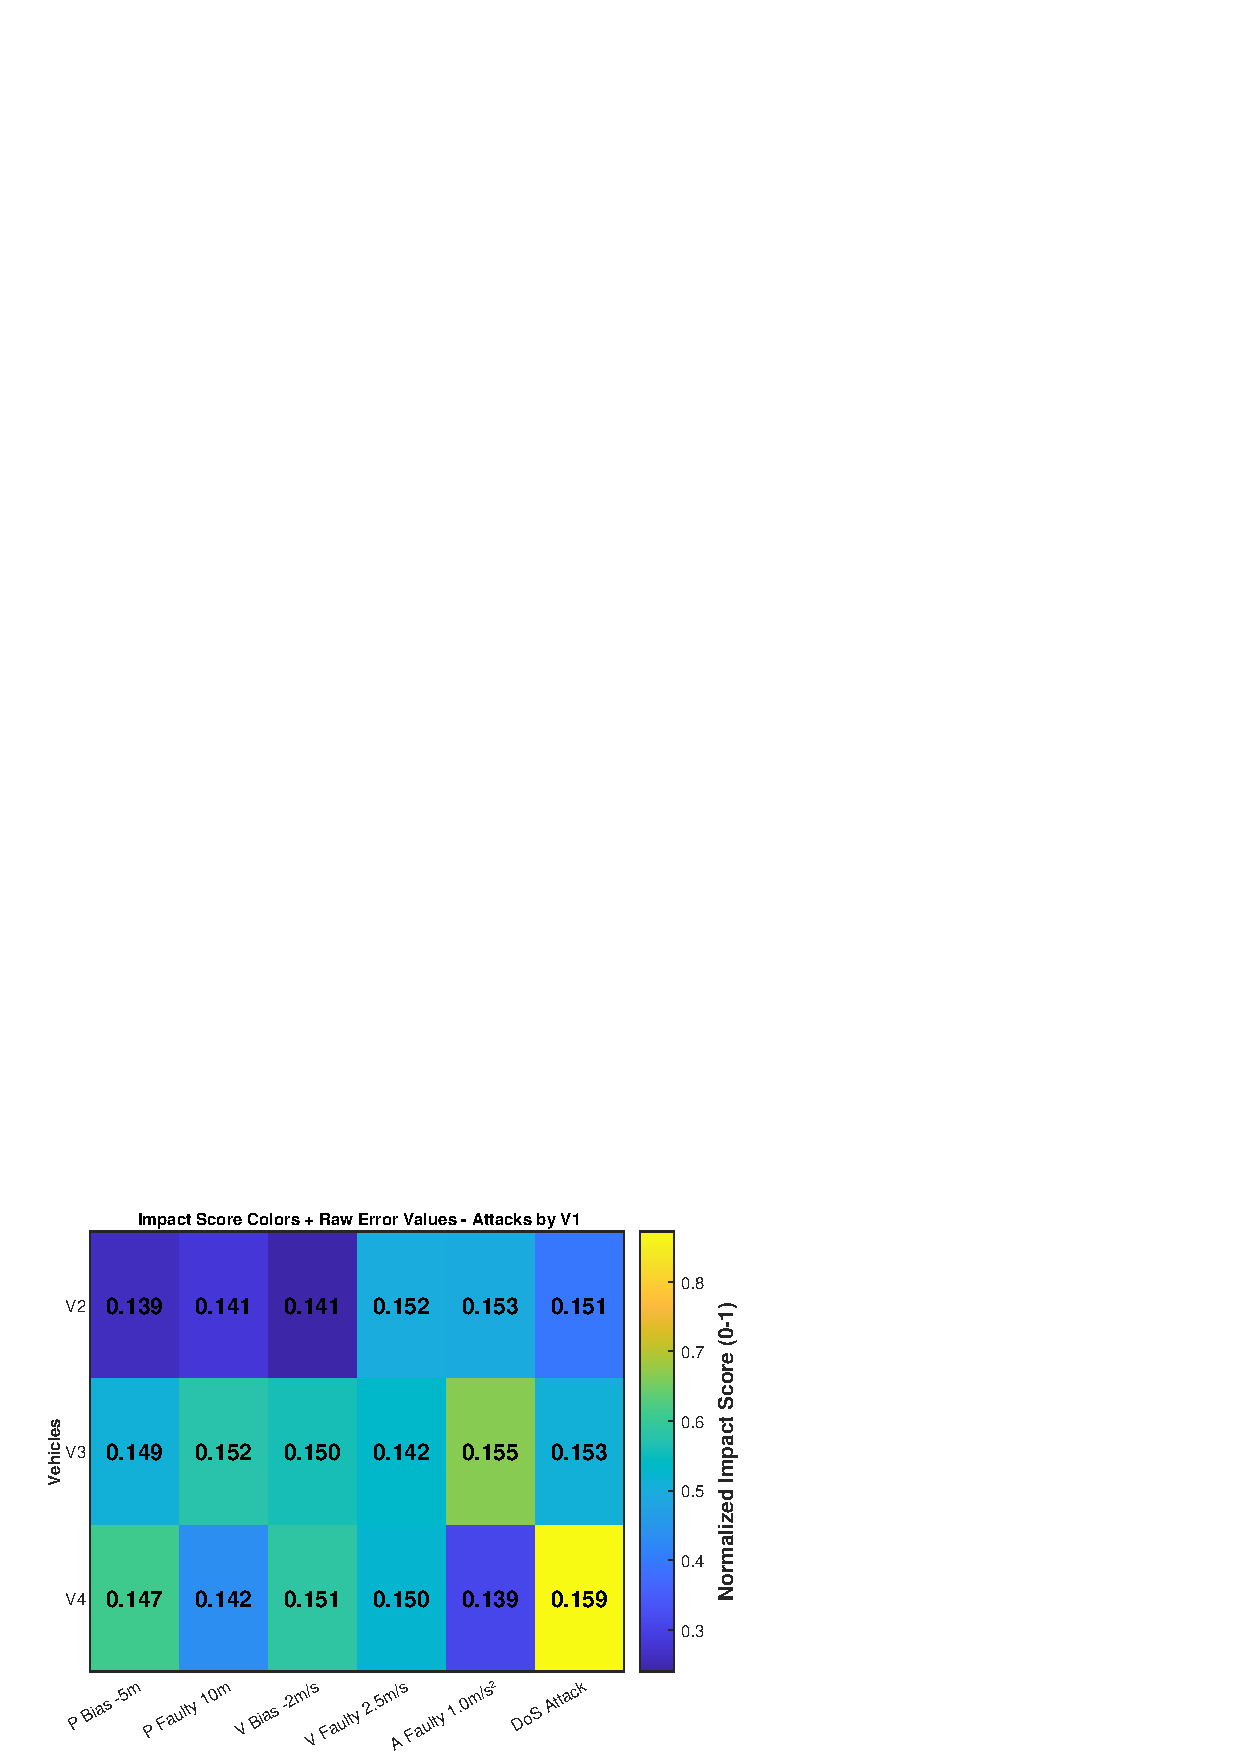
\includegraphics[width=\linewidth]{ch5/img/hybrid.jpg}
    \caption{Heatmap of normalized impact scores for all vehicles and attack cases.}
    \label{fig:hybird_heatmap}
\end{figure}


\begin{figure}[h!]
    \centering
    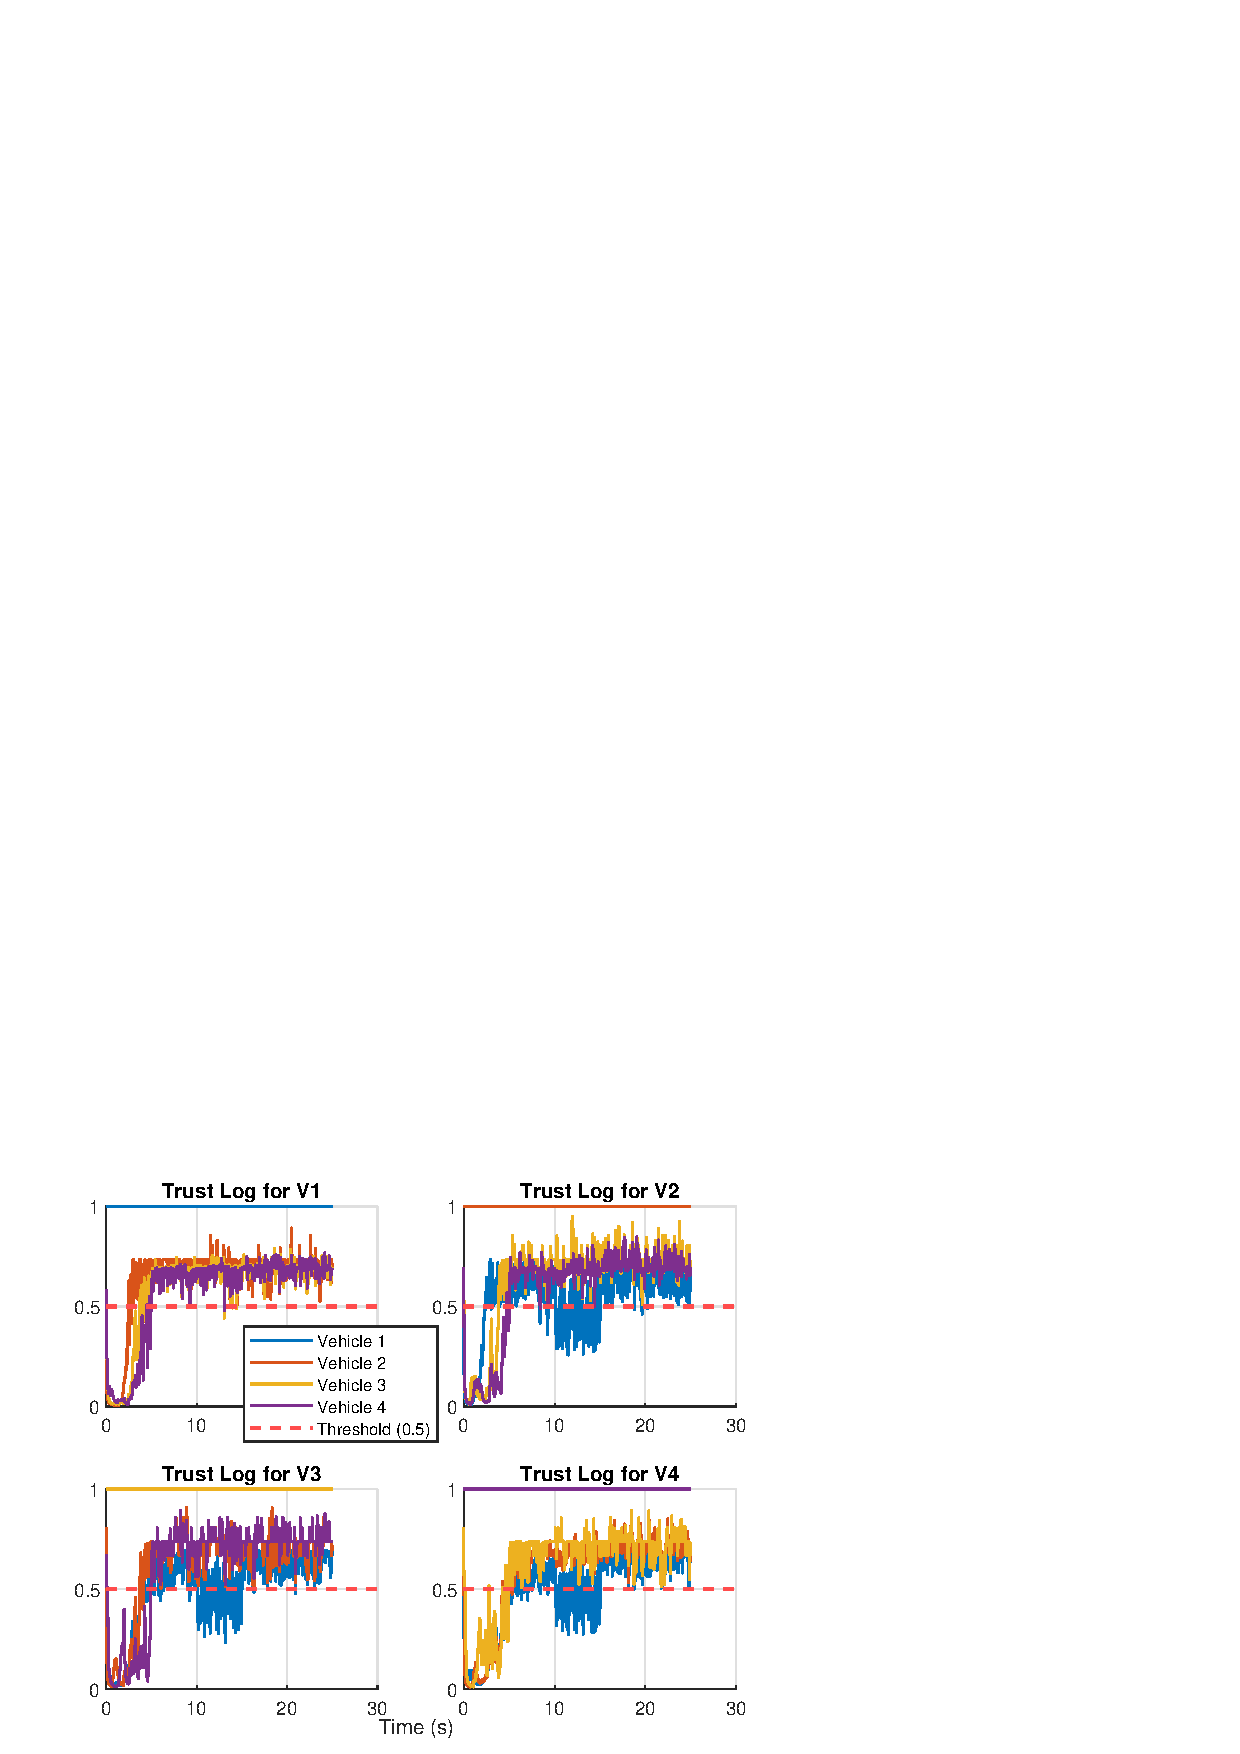
\includegraphics[width=\linewidth]{ch5/img/trust_all_new_huy.jpg}
    \caption{Trust score evolution during DoS attack ({\it\textbf{Case~6}}).}
    \label{fig:trust_Dos}
\end{figure}

In Figure~\ref{fig:trust_Dos}, the trust score evolution for the DoS attack (Case~6) is illustrated. During the attack period $[10, 15]$~s, these 3 vehicles (V2, V3, V4) exhibit a noticeable drop in trust values below the threshold of 0.5, indicating successful detection of the communication disruption. Once the attack ceases, the trust scores gradually recover, demonstrating the system ability to restore confidence and resume normal operation. This behavior confirms the effectiveness of the proposed trust mechanism in identifying and isolating malicious data in real time.






\subsection{Distributed State Estimation for Platoon Control}
% Introducing the platoon control framework using distributed state estimation
In this section, we present a platoon control framework that leverages distributed state estimation to enhance longitudinal control performance. The approach adopts a constant time headway spacing (CTHS) policy to maintain small inter-vehicle distances, improving traffic flow and safety. Two controllers are employed: an inner controller, based on the Intelligent Driver Model (IDM), for local longitudinal control using estimates from the local observer, and an outer controller, the Cooperative Adaptive Cruise Control (CACC), for distributed coordination using estimates from the distributed observer. These controllers are combined to form a robust final control strategy, balancing local responsiveness and platoon-wide consensus.

% Clarifying notation for state estimates
\subsubsection{Notation}

% For clarity, we define the notation for the estimated states used in the controllers:
% \begin{itemize}
%     \item \textbf{Local Observer ($\LO_i$)}: Each vehicle $i$ estimates its own state as $\hat{x}_0^{(i)} = [\hat{s}_0^{(i)}, \hat{v}_0^{(i)}, \hat{a}_0^{(i)}]^\top$, where $\hat{s}_0^{(i)}$, $\hat{v}_0^{(i)}$, and $\hat{a}_0^{(i)}$ are the estimated position, velocity, and acceleration of vehicle $i$, respectively.
%     \item \textbf{Distributed Observer ($\DO_i^{(j)}$)}: Each vehicle $i$ estimates the state of vehicle $j$ as $\hat{x}_i^{(j)} = [\hat{s}_i^{(j)}, \hat{v}_i^{(j)}, \hat{a}_i^{(j)}]^\top$, where $\hat{s}_i^{(j)}$, $\hat{v}_i^{(j)}$, and $\hat{a}_i^{(j)}$ are the estimated position, velocity, and acceleration of vehicle $j$ from the perspective of vehicle $i$.
% \end{itemize}

% Describing the inner controller: IDM
\subsubsection{Inner/Local Controller: Intelligent Driver Model (IDM)}
% Introducing the IDM and its purpose
The IDM is a car-following model that computes a vehicle's desired acceleration based on its own state and the relative state to its predecessor. Here, it serves as the inner controller for local longitudinal control, utilizing the local observer's estimate of the vehicle's own state, $\hat{x}_0^{(i)}$. The IDM acceleration for vehicle $i$ is given by:
\begin{equation}
    a_{\text{IDM},i} = \alpha \left[ 1 - \left( \frac{\hat{v}_0^{(i)}}{v_0} \right)^\delta - \left( \frac{s^*(\hat{v}_0^{(i)}, \Delta v_{i-1,i})}{s_{i-1,i}} \right)^2 \right],
\end{equation}
where:
\begin{itemize}
    \item $\hat{v}_0^{(i)}$ is the estimated velocity of vehicle $i$ from $\LO_i$.
    \item $s_{i-1,i} = s_{i-1} - s_i - L$ is the actual relative distance to the predecessor, with $L$ as the vehicle length (assuming direct sensor measurement for simplicity, as the query specifies IDM uses only local observer estimates, but relative distance typically requires predecessor data).
    \item $\Delta v_{i-1,i} = v_{i-1} - \hat{v}_0^{(i)}$ is the actual relative velocity, using the predecessor's true velocity $v_{i-1}$ from sensors.
    \item $s^*(\hat{v}_0^{(i)}, \Delta v_{i-1,i}) = s_0 + T \hat{v}_0^{(i)} + \frac{\hat{v}_0^{(i)} \Delta v_{i-1,i}}{2 \sqrt{\alpha \beta}}$ is the desired minimum gap.
    \item $\alpha$, $\beta$, $\delta$, $v_0$, $s_0$, and $T$ are model parameters: maximum acceleration, comfortable deceleration, free-flow exponent, desired velocity, minimum gap, and time headway, respectively.
\end{itemize}
% Noting the limitation and practical assumption
Since $\LO_i$ provides only $\hat{x}_0^{(i)}$ and not the predecessor's state, we assume vehicle $i$ uses sensor data (e.g., radar) for $s_{i-1,i}$ and $\Delta v_{i-1,i}$, consistent with standard IDM implementations, while adhering to the query's directive to use local observer estimates for the vehicle's own state.

% Describing the outer controller: CACC
\subsubsection{Cooperative Controller: Cooperative Adaptive Cruise Control (CACC)}
% Introducing the CACC and its cooperative purpose
The CACC enhances platoon coordination by leveraging information from multiple preceding vehicles via the distributed observer $\DO_{i}$. For vehicle $i$, the CACC control input is:
\begin{align}
    u_{\text{CACC},i}(k) = \sum_{j=1}^{i-1} [ \kappa_s \left( \hat{s}_i^{(j)}(k) - \hat{s}_0^{(i)}(k) - d_{i,j}(k) \right) \\ \notag +  \kappa_v \left( \hat{v}_i^{(j)}(k) -  \hat{v}_0^{(i)}(k) \right) + \kappa_a \left( \hat{a}_i^{(j)}(k) - \hat{a}_0^{(i)}(k) \right)]
\end{align}

where:
\begin{itemize}
    \item $\hat{s}_i^{(j)}(k)$, $\hat{v}_i^{(j)}(k)$, $\hat{a}_i^{(j)}(k)$ are the estimated position, velocity, and acceleration of vehicle $j$ from $\DO_i^{(j)}$.
    \item $\hat{s}_0^{(i)}(k)$, $\hat{v}_0^{(i)}(k)$, $\hat{a}_0^{(i)}(k)$ are the estimated position, velocity, and acceleration of vehicle $i$ from $\LO_i$ (included for consistency, though the query specifies distributed observer estimates for CACC).
    \item $d_{i,j}(k) = d + h \hat{v}_0^{(i)}(k)$ is the desired spacing between vehicles $i$ and $j$, with $d$ as a constant gap and $h$ as the time headway (for $j = i-1$, this aligns with the CTHS policy).
    \item $\kappa_s$, $\kappa_v$, $\kappa_a$ are control gains for position, velocity, and acceleration errors, respectively.
\end{itemize}
% Explaining the cooperative mechanism
This formulation ensures that vehicle $i$ adjusts its behavior based on the estimated states of all preceding vehicles, promoting consensus and stability across the platoon.

% Combining the controllers into a final strategy
\subsubsection{Final Controller}
% Defining the combined control input
The final control input integrates the IDM and CACC controllers to balance local and cooperative objectives. The target acceleration is:
\begin{equation}
    a_{\text{target},i} = (1 - \gamma(t)) a_{\text{IDM},i} + \gamma(t) u_{\text{CACC},i},
\end{equation}
where \(\gamma(t) \in [0,1]\) is a tuning parameter that is influenced by the opinion score mentioned in Section \ref{sec_trust_score}. For this context, we choose \(\gamma(t) = \min(\mathcal{O}_i)\).
% \begin{itemize}
%     \item $\gamma = 0$: Relies solely on IDM (local control).
%     \item $\gamma = 1$: Relies solely on CACC (cooperative control).
% \end{itemize}
% Applying a filter for smooth control
To prevent abrupt changes of the mixing 2 type controller, a first-order filter is applied:
\begin{equation}
    u_i(t) = u_i(t-1) + \tau_f (a_{\text{target},i} - u_i(t-1)),
\end{equation}
where $\tau_f$ is the filter time constant. 

% The vehicle's velocity is then updated as:
% \begin{equation}
%     v_i(t) = v_i(t-1) + u_i(t) \Delta t,
% \end{equation}
% with $\Delta t$ as the time step.

% Analyzing expected spacing for validation
\subsubsection{Expected Distance (Spacing)}
% Deriving steady-state spacing for evaluation
To validate the control strategy, we derive the expected steady-state spacing:
\begin{itemize}
    \item \textbf{IDM Steady-State Spacing}: When $a_{\text{IDM},i} = 0$ and $\Delta v_{i-1,i} = 0$:
    \[
    1 - \left( \frac{\hat{v}_0^{(i)}}{v_0} \right)^\delta = \left( \frac{s_0 + T \hat{v}_0^{(i)}}{s_{i-1,i}} \right)^2,
    \]
    yielding:
    \[
    s_{i-1,i} = \frac{s_0 + T \hat{v}_0^{(i)}}{\sqrt{1 - \left( \frac{\hat{v}_0^{(i)}}{v_0} \right)^\delta}}.
    \]
    \item \textbf{CACC Steady-State Spacing}: For the CTHS policy, when the platoon reaches consensus (all velocities equal), the spacing between vehicle $i$ and $i-1$ is:
    \[
    \boxed{s_i = d + \frac{h\,\hat{v}_0^{(i)}}{\,i-1}\,.}
    \]
\end{itemize}
% Explaining the validation process
These expressions allow comparison with simulation results, assessing the controllers' ability to maintain desired spacing under various conditions, including cyber-attacks.

\begin{figure}[h!]
    \centering
    \begin{subfigure}[t]{0.49\linewidth}
        \centering
        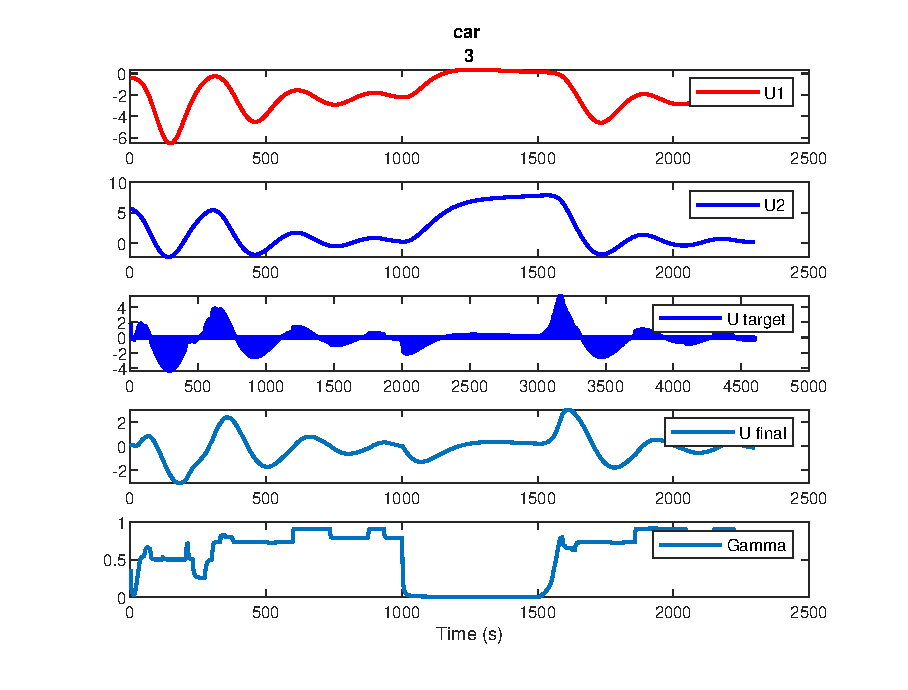
\includegraphics[width=1\linewidth]{ch5/img/controller_3.eps}
        % \caption{Compare with and without the local data exchange (Instance 1).}
        \label{fig:controller_3}
    \end{subfigure}
    \hfill
    \begin{subfigure}[t]{0.49\linewidth}
        \centering
        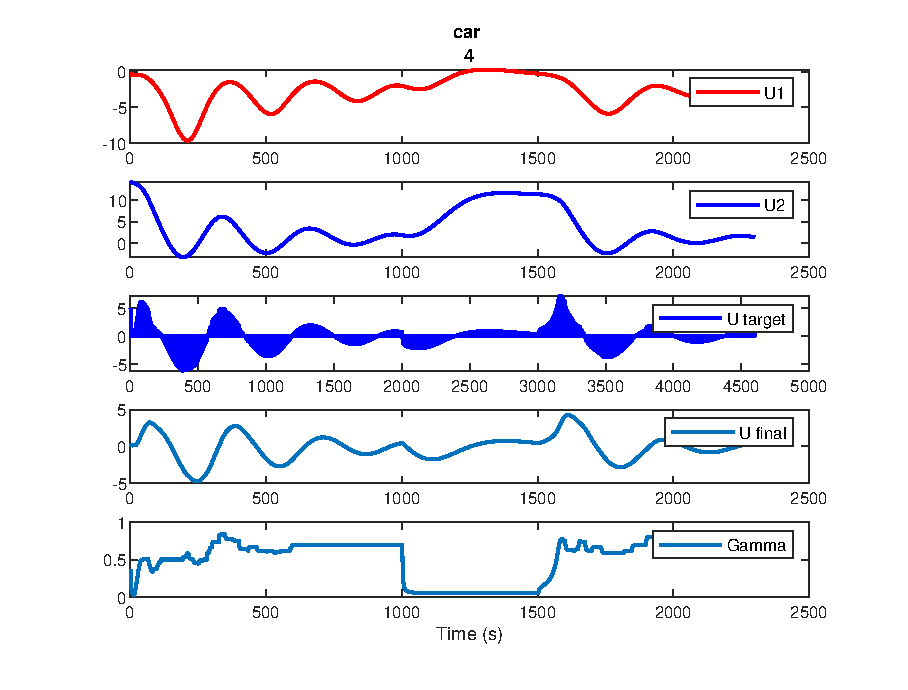
\includegraphics[width=1\linewidth]{ch5/img/controller_4.eps}
        % \caption{Compare with and without the local data exchange (Instance 2).}
        \label{fig:controller_4}
    \end{subfigure}
    
    \caption{Controller of vehicle 2 and 3.}
    \label{fig:controller_23}
\end{figure}


In figure \ref{fig:controller_23}, we can see the control input of vehicle 2 and 3, which is the acceleration of the vehicle. Smoothly switched between 2 controllers, and no abrupt change in the control input.
\begin{figure}
    \centering
    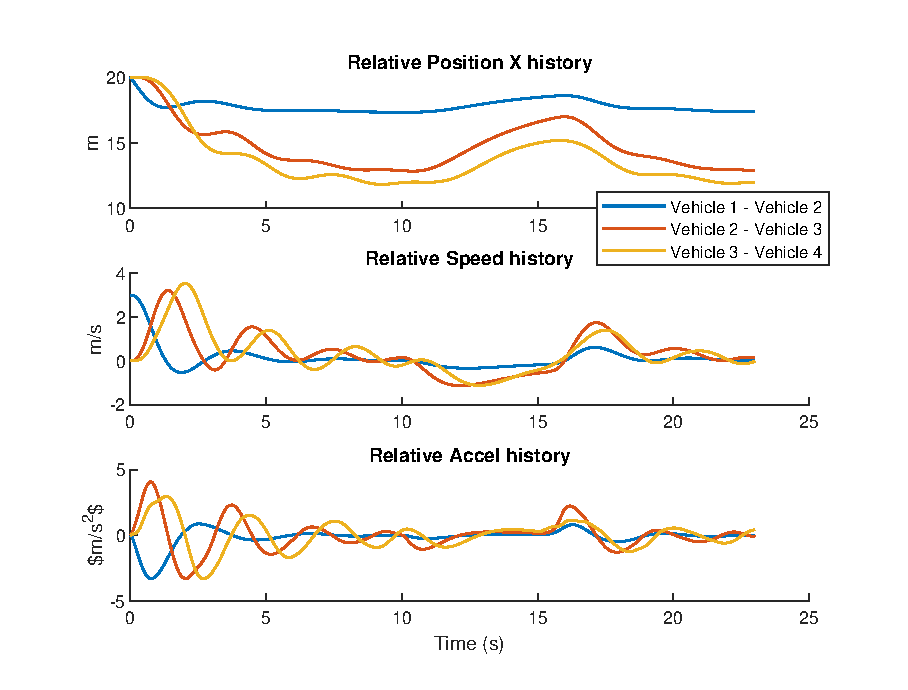
\includegraphics[width=0.8\linewidth]{ch5/img/relative_final_true.eps}
    \caption{Relative state of the vehicle in platoon}
    \label{fig:relative_final_true}
\end{figure}


In figure \ref{fig:relative_final_true}, we can see the relative state of the vehicle in platoon, which is the difference between the position of the vehicle and the position of its predecessor.
That prouve even in attack scenario, the vehicle can keep good distance No accident or crash happen in the platoon, which is a good sign of the robustness of the platoon control framework. 
Also that show the expected distance between the vehicle and its predecessor is maintained, which is the desired spacing in the platoon.


\section{Conclusion and Future Work}\label{sec_conclusion}
\vspace*{-0.2cm}
% Limitation – Estimating Malicious Vehicles
This paper presented a distributed observer-based platoon control framework capable of maintaining stability and safety under cyberattacks. The approach combines local and distributed observers with a trust evaluation mechanism to assess the reliability of inter-vehicle data, ensuring robust operation even with compromised nodes. 
%
%The proposed trust-based observer effectively protects the platoon by isolating malicious agents and preventing the propagation of corrupted data. However, it does not allow accurate estimation of the states of those malicious vehicles themselves. Once a vehicle's trust score falls below the threshold, its information is excluded from neighbor updates and is no longer corrected by trusted nodes. Consequently, its state estimate cannot converge to the true state. The framework thus prioritizes platoon safety and resilience over reconstructing the exact behavior of compromised vehicles a limitation shared by most existing distributed observer designs.
%

\subsection{Open Problems and Future Directions}
\vspace*{-0.2cm}
The analysis in this chapter focuses on stability and boundedness (ISS) under bounded disturbances and a trust-driven switching topology. Several open problems remain before such architectures can be made both sharper (less conservative) and more resilient in practice:
\begin{itemize}
    \item \textbf{Matrix-valued (channel-wise) trust weights.}
    In~\eqref{eq_observer}--\eqref{design_gain}, the coupling weights $w_{il}^{(j)}(t)$ are scalar and therefore apply the same attenuation to all state channels. A promising extension is to replace them with \emph{matrix} gains $W_{il}^{(j)}(t)\in\mathbb{R}^{n_x\times n_x}$ (e.g., diagonal or block-diagonal), allowing the trust mechanism to down-weight only the corrupted channels (e.g., acceleration) while preserving reliable channels (e.g., position). This leads to a matrix-weighted virtual Laplacian and stability conditions of the form
    $\|\mathcal{A}_{\mathrm{DO}}^{(j)}(t)\|_*\le \alpha<1$ for a suitably defined induced norm, or equivalently LMI-type contraction constraints on the lifted (block) error dynamics.

    \item \textbf{Trust/detection delay and rollback mechanisms.}
    In realistic networks, trust values are computed from time windows and may be delayed; consequently, false data can enter the distributed observer before a node is flagged, degrading the estimate. Moreover, abruptly cutting a node can temporarily reduce information flow and worsen estimation during the transition.
    A natural direction is to equip each host with a \emph{rollback buffer}: store a fixed window of past estimates and received packets. When the trust of a node drops below threshold, roll back to time $t-T_{\mathrm{w}}$ (window length) and re-propagate the observer using (i) only trusted neighbors and (ii) model-based prediction/local-observer anchoring to bridge the missing information. This resembles fixed-lag smoothing with trust-aware data rejection and could mitigate transient corruption while preserving stability, provided the reset/rollback map is bounded and updates satisfy a dwell-time or bounded-variation condition.

    \medskip
    \noindent\emph{Contamination rollback (compact recipe).}
    If a neighbor $l^{\star}$ is flagged at time $t$, undo the last $K$ steps by keeping a buffer of the \emph{innovation terms} appearing in~\eqref{eq_DO}. For each step $k$, store $\hat{x}_i^{(j)}(k)$ and
    \begin{align*}
    \eta_{il}^{(j)}(k) &\triangleq w_{il}^{(j)}(k)\big(\hat{x}_l^{(j)}(k)-\hat{x}_i^{(j)}(k)\big),\quad l\in\mathcal{N}_i,\\
    \eta_{i0}^{(j)}(k) &\triangleq w_{i0}^{(j)}(k)\big(\hat{x}_0^{(j)}(k)-\hat{x}_i^{(j)}(k)\big),
    \end{align*}
    as well as the input term $\hat{u}_j(k)$. When $l^{\star}$ is flagged, set $x\leftarrow\hat{x}_i^{(j)}(t-K)$ and replay for $k=t-K,\ldots,t-1$ using the same observer update but excluding $l^{\star}$ (or a malicious set $\mathcal{M}$):
    \begin{equation*}
    x \leftarrow A_{\text{b}}\Big(x + \sum_{l\in\mathcal{N}_i\setminus\mathcal{M}} \eta_{il}^{(j)}(k) + \eta_{i0}^{(j)}(k)\Big) + B_{\text{b}}\hat{u}_j(k),
    \end{equation*}
    and finally set $\hat{x}_i^{(j)}(t)\leftarrow x$.

    \item \textbf{Data-driven trust and learned uncertainty (with model-based safety layer).}
    Machine learning can be used to \emph{learn the mapping from signals to reliability}, while keeping the stability guarantee in the model-based layer by enforcing bounded weights. Concretely: (i) learn a calibrated trust score or anomaly probability from a feature vector built from innovation/residual signals (e.g., $\hat{x}_l^{(j)}-\hat{x}_i^{(j)}$, $\varepsilon_{i,l}^{(j)}$, packet age/loss, and consistency indicators), using change-point detection, self-supervised prediction, or lightweight sequence models; (ii) learn state-dependent covariance/uncertainty (heteroscedastic models) to adapt $\Sigma_{\text{local}}$ and thresholding; and (iii) implement the learned output only through a saturation/projection step that maps it to admissible weights satisfying Condition~(2) and preserving contraction in Condition~(3).
\end{itemize}

Future work will also focus on enhancing the trust mechanism by coupling it more closely with the controller, enabling trust evaluation for non-neighboring vehicles, and improving adaptability under dynamic communication topologies. 
We will also investigate machine-learning based trust estimation.
% \newpage
% \appendix
\chapter[Vehicle experiments and Board electronic]{Vehicle experiments and Board electronic}\label{chp6_chap}
\chaptermark{Vehicle experiments and Board electronic}

\objectif{This chapter reports the experimental validation workflow and the implementation results obtained on the Quanser QCar2/QLabs platform.
It first presents the virtual-to-real experimental methodology, the platform architecture (sensing, perception, V2V communication, software stack), and the longitudinal/lateral control loops used to reproduce cooperative driving.
Then, it details the observer and trust-aware distributed estimation pipeline, and summarizes the main results under nominal conditions and under representative cyber/communication attack scenarios.
Finally, this chapter introduces the custom embedded electronic board designed to host the proposed estimation and trust mechanisms on a real vehicle, and discusses the firmware validation and the integration roadmap.
}

%%%%%%%%%%%%%%%%%%%%%%%%%%%%%%%%%%%%%%%%%%%%%%%%%%%%%%%%%%%%%%%%%%%%%%%%%%%%%%%%%%%%%%%%%%%%%%%%%
\section{Vehicle Experiments }\label{chp6_sec_vehicle_experiments}
%%%%%%%%%%%%%%%%%%%%%%%%%%%%%%%%%%%%%%%%%%%%%%%%%%%%%%%%%%%%%%%%%%%%%%%%%%%%%%%%%%%%%%%%%%%%%%%%%

\subsection{Experimental methodology: from virtual validation to real trials}\label{chp6_subsec_methodology}
The experimental validation strategy follows a modular pipeline centered on (i) platoon modeling, (ii) cooperative control, (iii) distributed observation, and (iv) incremental validation on a realistic platform.
In practice, the workflow is decomposed into five phases:
\begin{itemize}
	\item \textbf{Phase 1 -- Environment setup:} configuration of the virtual environment under Ubuntu and deployment of the Quanser Virtual Environment container to connect QLabs and QCar2.
	\item \textbf{Phase 2 -- V2V communication and software architecture:} implementation of inter-vehicle communication via UDP and development of a modular Python architecture.
	\item \textbf{Phase 3 -- Longitudinal and lateral control:} two complementary control loops are implemented:
	(i) longitudinal control to regulate speed and inter-vehicle distance, and
	(ii) lateral control to track the road/trajectory.
	\item \textbf{Phase 4 -- Observer and trust system:} development of a distributed observer to estimate the fleet states even in presence of delays and information losses; integration of a trust system that weights the reliability of received data and dynamically adapts the fusion mechanism.
	\item \textbf{Phase 5 -- Full integration and real-time validation:} complete integration and real-time testing in QLabs; the transfer to physical scenarios on real QCar2 is prepared as a next step.
\end{itemize}

\begin{figure}[!ht]
	\centering
	% \fbox{\parbox{0.9\linewidth}{\vspace{1.6cm}\centering Placeholder for the virtual-to-real experimental workflow ("Figure 3" in the provided report).\vspace{1.6cm}}}
	\includegraphics[width=0.9\linewidth]{ch6/fig/Modular_Experimental_Phases.png}
    \caption{Modular Experimental Phases.}
	\label{fig:ch6_modular_Experimental_Phases}
\end{figure}

The objective of the real-trial preparation is to design an \emph{embedded intelligent soft sensor} able to estimate non-measured quantities and detect disturbances related to cyberattacks and/or sensor faults.
This embedded soft sensor associates perception measurements to surrounding vehicles, reconstructs critical variables, and distinguishes physical anomalies from malicious perturbations.


\begin{figure}[!ht]
	\centering
	% \fbox{\parbox{0.9\linewidth}{\vspace{1.6cm}\centering Placeholder for the virtual-to-real experimental workflow ("Figure 3" in the provided report).\vspace{1.6cm}}}
	\includegraphics[width=0.9\linewidth]{ch6/fig/experimental_workflow.png}
    \caption{Experimental workflow for the virtual validation on QLabs/QCar2 and preparation of real trials.}
	\label{fig:ch6_workflow}
\end{figure}
Beyond the modular phases described above, 
the experiments rely on a coordinated workflow that links code development, 
simulation, and real-world testing. 
A containerized development environment is used to write and package the Python control and estimation code. 
Once a new controller or observer is ready, the container sends the code to a Graphical Ground Station. 
This application acts as the central hub for the experiments: it runs the cooperative control and planning algorithms, visualizes trajectories and state estimates in real time, 
and forwards commands to the test platform. 
When working with the QLabs simulator, the ground station interfaces with the QLabs Virtual Environment, which is a digital twin of the physical QCar platform. 
The virtual QCar behaves the same way as the real hardware and exposes the same sensors and actuators, so control software can be measured and tested in simulation before deployment.

During a simulation trial, the ground station sends high‑level control commands (e.g., desired speed and spacing) to the virtual environment and receives simulated sensor data and vehicle states. 
This allows the researcher to verify the platoon behaviour, tune the cooperative adaptive cruise control and look‑ahead steering loops, and adjust observer parameters. 
Because the digital twin mirrors the physical self‑driving car studio, the same code can then be executed on the real QCar with minimal changes. 
In physical tests, the ground station sends visual plots and user commands to the vehicle while logging the on‑board measurements, estimated distances and trust indicators. 
The logs collected during real trials are sent back to the containerized development environment, where they are analysed to refine the models and software. This feedback loop—code development → ground‑station execution → virtual trials → physical trials → log analysis—enables safe, incremental validation: controllers and observers are first validated in a realistic digital twin, then applied to the real vehicle. Bridging and blending code between the virtual and physical platforms allows researchers to explore new scenarios and behaviours while ensuring that the resulting algorithms are robust when transferred to hardware.

\section{Quanser QCar2/QLabs experimental platform}\label{chp6_sec_platform}

\subsection{Virtual environment and scenario definition}\label{chp6_subsec_virtual_env}
The QLabs environment is configured with two connected vehicles: a \emph{leader} vehicle tracking a predefined closed-loop trajectory and a \emph{follower} vehicle reproducing cooperative platoon behavior.
The leader trajectory is defined via a set of waypoints that form a closed loop.
In the reported experiments, a desired speed of $0.3\,\mathrm{m/s}$ is selected to generate a smooth and repeatable reference motion for the follower.
The scenario includes typical road elements (ground, walls, pedestrian crossing), making it closer to real driving conditions.

\begin{figure}[!ht]
	\centering
	\fbox{\parbox{0.9\linewidth}{\vspace{1.6cm}\centering Placeholder for the QLabs environment configuration and the selected waypoints ("Figures 5--6" in the provided report).\vspace{1.6cm}}}
	\caption{QLabs scenario and example of selected waypoints for the leader vehicle.}
	\label{fig:ch6_qlabs_waypoints}
\end{figure}

\subsection{Measurements and perception pipeline}\label{chp6_subsec_measurements}
Designing trust-aware distributed estimation requires a clear definition of the measurements and metadata available on the QCar2 platform.
In this work, the data sources include: onboard sensors, perception modules (LiDAR-camera fusion), and V2V exchanged states.
Table~\ref{tab:ch6_qcar_measurements} summarizes the measurements used in the reported experiments.

\begin{table}[!ht]
	\centering
	\caption{Summary of measurements and metadata available on QCar2/QLabs used for control, estimation, and trust evaluation.}
	\label{tab:ch6_qcar_measurements}
	\renewcommand{\arraystretch}{1.15}
	\begin{tabular}{p{0.21\linewidth} p{0.26\linewidth} p{0.24\linewidth} p{0.25\linewidth}}
		\hline
			\textbf{Category} & \textbf{Measurement / Metadata} & \textbf{Source} & \textbf{Usage} \\
		\hline
		Onboard sensors (raw) & Position $(x,y)$ and timestamp & QLabs virtual GPS (GPSSync API) & Time alignment and trajectory registration \\
		Onboard sensors (raw) & Acceleration and angular rate & IMU (accelerometers, gyros) & Instantaneous vehicle dynamics \\
		Onboard sensors (raw) & 2D point cloud & LiDAR (RPLiDAR A2, $12\,\mathrm{m}$ range) & 360$^\circ$ obstacle sensing \\
		Onboard sensors (raw) & RGB / depth images & Cameras (Intel RealSense D435 and CSI 360$^\circ$) & Visual perception \\
		Onboard sensors (raw) & Wheel speed and steering angle & Motor encoder and steering servo & Inputs for longitudinal/lateral control \\
		Derived kinematics & Position, orientation $(\psi)$ & QLabs global state & Absolute vehicle state in the map \\
		Derived kinematics & Longitudinal speed $(v)$ & Encoder + Kalman filter & Smoothed speed estimate \\
		Derived kinematics & Longitudinal acceleration $(a)$ & Derivative of $v$ (Kalman) or IMU & Longitudinal acceleration estimate \\
		Cooperative variables & Inter-vehicle distance $(d)$ & LiDAR-camera fusion pipeline & Reliable distance for cooperative control \\
		Cooperative variables & Relative speed $(\Delta v)$ & Temporal derivative of $d$ & Rate of change of inter-vehicle gap \\
		V2V metadata & Neighbor states $(p,v,a)$ & Periodic V2V messages & Cooperation / distributed estimation \\
		V2V metadata & Link quality & Packet loss rate, delays & Communication reliability for trust \\
		\hline
	\end{tabular}
\end{table}

Two critical quantities for cooperative control and trust assessment are the inter-vehicle distance $d$ and the relative speed $\Delta v$.
They are obtained via a LiDAR-camera fusion pipeline, which can be summarized as follows:
\begin{itemize}
	\item Image segmentation: YOLOv8-seg is used to extract object masks (vehicles, pedestrians).
	\item Post-processing: mask erosion reduces false positives.
	\item LiDAR projection: 3D LiDAR points are projected into the image plane using intrinsic/extrinsic calibration matrices.
	\item Data association: projected points are associated to segmented objects, yielding a 2D-3D coupling.
	\item Spatial clustering: DBSCAN filters and groups fused points.
	\item 3D estimation: PCA computes 3D bounding boxes and relative positions.
	\item Final quantities: distance $d$ is deduced from relative position; relative speed is obtained from time-derivative of $d$.
\end{itemize}

% \begin{figure}[!ht]
% 	\centering
% 	\fbox{\parbox{0.92\linewidth}{\vspace{1.7cm}\centering Placeholder for LiDAR bird-eye view and camera fusion view ("Figures 7--8" in the provided report).\vspace{1.7cm}}}
% 	\caption{Illustration of LiDAR-camera fusion for inter-vehicle distance estimation.}
% 	\label{fig:ch6_lidar_camera_fusion}
% \end{figure}

% In the reported example, the estimated distances displayed in real time include values such as $d \approx 8\,\mathrm{m}$ and $d \approx 22\,\mathrm{m}$.
% These results show that the cooperative variables $(d,\Delta v)$ do not come from raw sensors only, but from a multimodal perception chain that combines vision and LiDAR.

\subsection{V2V communication and modular software architecture and Attack design}\label{chp6_subsec_v2v}
\subsubsection{Design of V2V communication}\label{chp6_subsubsec_v2v_design}
Beyond control and estimation algorithms, the overall system requires a robust communication layer.
The V2V stack is organized into three functional layers, as illustrated in Figure~\ref{fig:ch6_v2v_stack}:
\begin{enumerate}
	\item \textbf{Application layer}: high-level cooperative functions (platoon controller, distributed observer, trust manager) consume and produce vehicle state messages.
	\item \textbf{Session layer}: handles message reliability through acknowledgments (ACK/NACK), periodic heartbeats for neighbor-presence detection, and a virtual-GPS-based time synchronization service that timestamps every packet.
	\item \textbf{Transport layer}: UDP sockets transmit and receive datagrams at a fixed period (typically $T_s = 100\,\mathrm{ms}$). Separate threads handle transmission and reception to avoid blocking.
\end{enumerate}

At each communication period, a vehicle broadcasts a state packet containing:
\begin{itemize}
	\item vehicle identifier ($id$);
	\item position $(x,y)$ and heading $\psi$;
	\item longitudinal speed $v$ and acceleration $a$;
	\item synchronized timestamp $t$.
\end{itemize}
When a packet is received, an ACK is returned to the sender; if no ACK arrives within a timeout, the message is flagged as lost.
In parallel, a heartbeat mechanism periodically checks for missing neighbors: if no message (nor heartbeat) is received from a neighbor for a configurable interval, that neighbor is marked as unavailable and excluded from the cooperative estimation until communication resumes.
These mechanisms ensure temporal consistency and data integrity, which are prerequisites for the distributed observer and trust framework.

% ============================================================
% DIAGRAM SPECIFICATION FOR FIGURE ch6_v2v_stack
% ------------------------------------------------------------
% Create a vertical block diagram with three stacked layers:
%
%   ┌─────────────────────────────────────────────────────┐
%   │              APPLICATION LAYER                      │
%   │  ┌──────────┐  ┌──────────────┐  ┌──────────────┐   │
%   │  │ Platoon  │  │ Distributed  │  │    Trust     │   │
%   │  │Controller│  │  Observer    │  │   Manager    │   │
%   │  └────┬─────┘  └──────┬───────┘  └──────┬───────┘   │
%   └───────┼───────────────┼─────────────────┼───────────┘
%           │  state msgs   │                 │
%           ▼               ▼                 ▼
%   ┌─────────────────────────────────────────────────────┐
%   │               SESSION LAYER                         │
%   │  ┌──────────┐  ┌──────────────┐  ┌──────────────┐   │
%   │  │ ACK/NACK │  │  Heartbeat   │  │ GPS Time     │   │
%   │  │ Handler  │  │   Manager    │  │   Sync       │   │
%   │  └────┬─────┘  └──────┬───────┘  └──────┬───────┘   │
%   └───────┼───────────────┼─────────────────┼───────────┘
%           │  UDP pkts     │                 │
%           ▼               ▼                 ▼
%   ┌─────────────────────────────────────────────────────┐
%   │              TRANSPORT LAYER (UDP)                  │
%   │         ┌───────────┐    ┌───────────┐              │
%   │         │  TX Thread│    │  RX Thread│              │
%   │         └─────┬─────┘    └─────┬─────┘              │
%   └───────────────┼────────────────┼────────────────────┘
%                   │                │
%                   ▼                ▼
%              ══════════════════════════
%                  Wireless Channel
%              ══════════════════════════
% ============================================================

\begin{figure}[!ht]
	\centering
	% \fbox{\parbox{0.92\linewidth}{\vspace{1.7cm}\centering Placeholder for V2V communication stack diagram (see LaTeX comments above for specification).\vspace{1.7cm}}}
	\includegraphics[width=0.7\linewidth]{ch6/fig/V2V_achi.png}
	\caption{Layered architecture of the V2V communication stack used in the QLabs experiments.}
	\label{fig:ch6_v2v_stack}
\end{figure}

\subsubsection{Attack injection mechanism}\label{chap6_subsubsec_attack_insert}
To evaluate the robustness of the distributed observer and trust framework under adversarial conditions, a configurable \emph{attack injector} is integrated into the communication layer.
The injector intercepts outgoing or incoming V2V packets and applies one of several perturbation models before the data reach the application layer.
Figure~\ref{fig:ch6_attack_injector} illustrates the injection pipeline.

\paragraph{Injection modes.}
Three attack families are supported:
\begin{enumerate}
	\item \textbf{Bias injection}: a constant offset $\delta$ is added to one or more state variables (e.g., $\tilde{v} = v + \delta_v$).
	\item \textbf{Random fault}: with probability $p$, the transmitted value is replaced by a random sample drawn from a uniform distribution of configurable intensity.
	\item \textbf{Data drop (DoS)}: with probability $p_{drop}$, the packet is discarded entirely, simulating a denial-of-service or severe packet-loss scenario.
\end{enumerate}

\paragraph{Injection parameters.}
Each attack scenario is defined by:
\begin{itemize}
	\item \emph{attacker ID}: the vehicle whose outgoing messages are corrupted;
	\item \emph{target variables}: which state components are affected (position, velocity, acceleration, or all);
	\item \emph{attack window}: the time interval $[t_{start}, t_{end}]$ during which the attack is active;
	\item \emph{attack parameters}: bias magnitude $\delta$, fault intensity, or drop probability $p_{drop}$.
\end{itemize}
The injector can operate transparently (victim vehicles are unaware) or be logged for post-experiment analysis.
This flexibility enables systematic benchmarking of the trust-aware estimation framework across a wide range of adversarial conditions (see Table~\ref{tab:ch6_attack_scenarios} for the specific scenarios used in this work).

% ============================================================
% DIAGRAM SPECIFICATION FOR FIGURE ch6_attack_injector
% ------------------------------------------------------------
% Create a horizontal flow diagram showing the attack injection point:
%
%   ┌────────────┐      ┌──────────────────────────────┐      ┌────────────┐
%   │  Sensor /  │      │       ATTACK INJECTOR        │      │ Application│
%   │  Estimator ├─────►│  ┌─────────────────────────┐ ├─────►│   Layer    │
%   │  (Sender)  │      │  │ Mode selector:          │ │      │ (Receiver) │
%   └────────────┘      │  │  • Bias injection       │ │      └────────────┘
%                       │  │  • Random fault         │ │
%        outgoing       │  │  • Packet drop (DoS)    │ │        corrupted /
%        V2V packet     │  └─────────────────────────┘ │        clean packet
%                       │                              │
%                       │  Parameters:                 │
%                       │   - attacker ID              │
%                       │   - target variables         │
%                       │   - time window [t_s, t_e]   │
%                       │   - δ, intensity, p_drop     │
%                       └──────────────────────────────┘
%
% Use color coding:
%   • Green arrow = clean packet path (bypass)
%   • Red arrow   = corrupted packet path
% ============================================================

\begin{figure}[!ht]
	\centering
	% \fbox{\parbox{0.92\linewidth}{\vspace{1.7cm}\centering Placeholder for attack injector pipeline diagram (see LaTeX comments above for specification).\vspace{1.7cm}}}
	\includegraphics[width=0.9\linewidth]{ch6/fig/attack_injector.png}
	\caption{Attack injection mechanism integrated into the V2V communication layer.}
	\label{fig:ch6_attack_injector}
\end{figure}

\section{Control architecture}\label{chp6_sec_control}

\subsection{Longitudinal control: cooperative cruise control}\label{chp6_subsec_longitudinal}
The longitudinal control loop is based on cooperative adaptive cruise control (CACC) to regulate both velocity and inter-vehicle spacing.
The control input combines locally measured quantities (e.g., speed/acceleration) with cooperative information received via V2V (e.g., predecessor acceleration), and relies on the perception-derived distance $d$ and relative speed $\Delta v$.
This chapter focuses on the experimental integration and validation aspects; the detailed CACC modeling and resilient observer-based compensation are developed in earlier chapters.

\subsection{Lateral control: extended look-ahead to reduce corner cutting}\label{chp6_subsec_lateral}
In curves, follower vehicles tend to exhibit \emph{corner cutting} (reduced turning radius compared to the leader), which can induce lateral offsets and affect the effective inter-vehicle spacing.
To mitigate this effect, an Extended Look-Ahead Controller (ELC) is implemented.
The idea is to define a virtual pursuit point $P^*$ located ahead of the preceding vehicle by a look-ahead distance $d_{LA}$ and laterally shifted by $d_{lat}$.
The follower then computes its steering command using this virtual target rather than the preceding vehicle's center of gravity.
This improves curve tracking and helps maintain the spacing policy (e.g., constant time-gap) in both straight and curved roads.

\begin{figure}[!ht]
	\centering
	\fbox{\parbox{0.92\linewidth}{\vspace{1.7cm}\centering Placeholder for corner-cutting comparison without/with look-ahead control ("Figures 10--11" in the provided report).\vspace{1.7cm}}}
	\caption{Effect of extended look-ahead on corner cutting in curves.}
	\label{fig:ch6_corner_cutting}
\end{figure}

% \section{Observer-based estimation and trust-aware distributed fusion}\label{chp6_sec_observers_trust}

% \subsection{Two-layer observation architecture}\label{chp6_subsec_observer_arch}
% Estimation is used to reconstruct states that are not directly measured with sufficient accuracy and to maintain robustness under noisy or missing data.
% Two complementary observation layers are implemented:
% \begin{itemize}
% 	\item \textbf{Local observer} (per-vehicle): estimates the vehicle state $x_i(t)$ from local measurements $y_i(t)$.
% 	\item \textbf{Distributed observer} (cooperative): each vehicle $i$ reconstructs states of other vehicles $j$ by combining its local observer outputs with V2V information from neighbors $\mathcal{N}_i$.
% \end{itemize}
% Under graph connectivity and appropriate gain choices, the distributed estimation converges to the true fleet state (as reported in the provided experimental document).

% \begin{figure}[!ht]
% 	\centering
% 	\fbox{\parbox{0.92\linewidth}{\vspace{1.7cm}\centering Placeholder for the two-layer observation/communication architecture ("Figure 12" in the provided report).\vspace{1.7cm}}}
% 	\caption{Two-layer estimation architecture: local observers and V2V-based distributed fusion.}
% 	\label{fig:ch6_two_layer_arch}
% \end{figure}

% \subsection{Nominal results (no attack)}\label{chp6_subsec_nominal_results}
% In nominal conditions, the local observer estimates are consistent with the GPS reference trajectories.
% The reported comparisons show that positions $(x,y)$, heading $\psi$, and longitudinal speed $v$ are accurately reconstructed despite encoder noise.
% Moreover, distributed observers enable each vehicle to reconstruct the full fleet state (trajectories and speed profiles) from V2V exchanges.
% These nominal results provide a baseline reference before introducing faulty or adversarial scenarios.

% \begin{figure}[!ht]
% 	\centering
% 	\fbox{\parbox{0.92\linewidth}{\vspace{1.7cm}\centering Placeholders for local-observer vs GPS plots and distributed fleet estimates ("Figures 13--18" in the provided report).\vspace{1.7cm}}}
% 	\caption{Nominal estimation results: local observer tracking of GPS and distributed reconstruction of fleet states.}
% 	\label{fig:ch6_nominal_estimation}
% \end{figure}

% \subsection{Trust framework integration}\label{chp6_subsec_trust}
% To increase resilience against compromised neighbors and communication faults, a trust framework is integrated into the distributed observer.
% Trust is computed from both local kinematic consistency and global consistency of distributed estimates:
% \begin{itemize}
% 	\item \textbf{Local evaluation functions:}
% 	\begin{itemize}
% 		\item \texttt{evaluate\_velocity()}: checks consistency between reported speed and observed displacement.
% 		\item \texttt{evaluate\_distance()}: compares reported position with locally measured inter-vehicle distance.
% 		\item \texttt{evaluate\_acceleration()}: evaluates whether speed variations are dynamically plausible.
% 	\end{itemize}
% 	\item \textbf{Global evaluation functions:}
% 	\begin{itemize}
% 		\item \texttt{gamma\_cross()}: measures coherence between a vehicle's global fleet estimates and observed data.
% 		\item \texttt{gamma\_local()}: checks if neighbors' local estimates match the ego vehicle perception.
% 	\end{itemize}
% \end{itemize}

% The \emph{local trust} is computed as a product of local consistency terms:
% \[
% 	LT = (\text{velocity})\times(\text{distance})\times(\text{acceleration}).
% \]
% The \emph{global trust} evaluates the reliability of the information a vehicle shares about the rest of the fleet:
% \[
% 	DT = \gamma_{cross}\times\gamma_{local}.
% \]
% The final combined trust score for vehicle $j$ is defined as
% \[
% 	O_j = DT\times LT.
% \]
% Based on this score, the set of trusted neighbors is updated online according to a simple thresholding rule:
% \[
% 	\mathcal{N}_i(t) = \{ j\in\mathcal{N}_i: O_j>0.5\}.
% \]
% Communication weights are then dynamically adapted as a function of the number of trusted neighbors.
% In particular, a normalized weight is maintained even when only a few neighbors are trusted, using a lower bound $\kappa$ to preserve connectivity.

% \begin{figure}[!ht]
% 	\centering
% 	\fbox{\parbox{0.92\linewidth}{\vspace{1.7cm}\centering Placeholders for trust impact heatmap and trust score evolution during DoS ("Figures 19--20" in the provided report).\vspace{1.7cm}}}
% 	\caption{Trust framework results: normalized impact scores and trust score evolution under DoS.}
% 	\label{fig:ch6_trust_results}
% \end{figure}

\subsection{Attack scenarios and quantitative summary}\label{chp6_subsec_attack_scenarios}
In the reported virtual experiments, the leader vehicle (ID 1) behaves as the attacker between $t=5\,\mathrm{s}$ and $t=10\,\mathrm{s}$.
Several scenarios are considered, including bias injection, random faults, and DoS-like packet drops on position/velocity/acceleration.

\begin{table}[!ht]
	\centering
	\caption{Attack scenarios used to evaluate the trust-aware estimation framework (leader ID 1 attacks other vehicles during $t\in[5,10]\,\mathrm{s}$).}
	\label{tab:ch6_attack_scenarios}
	\renewcommand{\arraystretch}{1.15}
	\begin{tabular}{c p{0.26\linewidth} p{0.26\linewidth} p{0.28\linewidth}}
		\hline
            \textbf{Case} & \textbf{Attack method} & \textbf{Parameter(s)} & \textbf{Target (data)} \\
		\hline
		1 & Bias & $-5\,\mathrm{m}$ & Position \\
		2 & Random fault & intensity $=10$, $p=0.3$ & Position \\
		3 & Bias & $-2\,\mathrm{m/s}$ & Velocity \\
		4 & Random fault & intensity $=2.5$, $p=0.3$ & Velocity \\
		5 & Random fault & intensity $=1.0$, $p=0.3$ & Acceleration \\
		6 & Data drop (DoS) & $p_{drop}=0.5$ & Position, velocity, acceleration \\
		\hline
	\end{tabular}
\end{table}

Two indicators are used to quantify the effects of the attacks: (i) a combined raw error capturing deviations on distance, speed, and acceleration estimates; and (ii) a normalized impact score obtained by dividing the combined error by the maximum error observed across scenarios.
Among the considered scenarios, the DoS attack (Case~6) yields the highest normalized impact score ($0.872$), confirming it as the most severe perturbation.
Conversely, the velocity bias attack (Case~3, bias $=-2\,\mathrm{m/s}$) yields the lowest reported impact score ($0.240$), indicating a limited effect on the overall platoon stability.
In terms of vehicle sensitivity, the reported results show that vehicle $V4$ is the most affected (max impact $0.872$), whereas vehicle $V2$ is the most resilient with the lowest average impact score ($0.362$).
Finally, the trust score evolution under DoS shows a clear drop below the $0.5$ threshold during the perturbation interval, followed by progressive recovery after the attack ends.

\section{Custom embedded electronic board for future onboard deployment}\label{chp6_sec_board}

\subsection{Motivation and design objectives}\label{chp6_subsec_board_motivation}
To move from simulation-based validation / small-scale experiments to real trials, the project includes the design of a dedicated embedded electronic board.
The objective is not only to ``run the code on hardware'', but to provide an integration-ready platform where sensing, communication, timing, and basic cyber-resilience can be validated under realistic constraints.
In this thesis, the board is envisioned as an embedded \emph{intelligent soft sensor}: it reconstructs non-measured variables, monitors the consistency of cooperative data, and exports reliable state and trust indicators to higher-level decision and control.

From a system engineering viewpoint, the design targets four key objectives:
\begin{itemize}
	\item \textbf{Real-time execution:} guarantee deterministic execution of periodic estimation and control-related computations (e.g., $\approx 100\,\mathrm{Hz}$ loops as used in the experimental software stack), with bounded jitter.
	\item \textbf{Multi-interface sensing and synchronization:} acquire heterogeneous data streams (inertial, positioning/time reference, and auxiliary sensors) and ensure time alignment through timestamping.
	\item \textbf{V2V-ready communication:} support low-latency exchange of compact state messages and metadata (packet loss, delay indicators) required by the distributed observer and trust evaluation.
	\item \textbf{Robustness and diagnosability:} provide a hardware and firmware structure that supports fault detection, health monitoring, and graceful degradation when sensors or communications are unavailable.
\end{itemize}

Compared with a purely PC-based ground-station deployment, the embedded approach also addresses practical constraints that become critical on a vehicle: compactness and wiring reduction, controlled power distribution, electromagnetic compatibility (EMC), and reliable boot/execution behavior.
The overall role of the board is therefore to acquire onboard sensing data, exchange information with neighboring vehicles, fuse local and remote information, and publish consolidated variables (including trust indicators) to the vehicle-level decision and control system.

\subsection{Architecture and PCB design}\label{chp6_subsec_board_hw}
The development process is structured into four phases: (i) functional needs analysis and block-architecture definition, (ii) electronic CAD design, (iii) prototyping and embedded programming, and (iv) experimental verification with rigorous test protocols.
The design identifies the required sensors, the target microcontroller family, and the relevant communication protocols, including \textbf{SPI}, \textbf{I$^2$C}, \textbf{UART}, and \textbf{Wi-Fi 6}.
The electronic design is implemented in KiCad and routed on a \textbf{4-layer PCB}, which offers two main benefits: (i) dedicated reference planes to control return paths and reduce EMI, and (ii) improved power distribution and decoupling compared with 2-layer prototypes.

\paragraph{Functional blocks.}
At a high level, the board architecture (Figure~\ref{fig:ch6_board_design}) can be described as a composition of:
\begin{itemize}
	\item a \textbf{real-time processing unit} (microcontroller + memory resources) responsible for scheduling tasks, running the embedded observer/trust logic, and managing peripherals;
	\item a \textbf{communication subsystem} supporting short-range V2V exchange (Wi-Fi) and wired diagnostic/telemetry links (UART);
	\item a \textbf{sensing and timing subsystem} interfacing inertial and positioning/time-reference signals through SPI/I$^2$C/UART, and providing timestamping for data consistency;
	\item a \textbf{power subsystem} that converts the vehicle supply to regulated rails for digital logic and RF modules, with attention to inrush current, ripple, and protection.
\end{itemize}

\paragraph{Electrical and layout considerations.}
Beyond functional connectivity, the PCB is designed to be compatible with an onboard environment where noisy actuators, switching regulators, and RF emissions may coexist.
The main layout guidelines are summarized below:
\begin{itemize}
	\item \textbf{Power integrity:} short decoupling loops close to IC supply pins, separation of noisy switching nodes from sensitive analog/RF areas, and adequate bulk capacitance for transient loads.
	\item \textbf{Grounding and return paths:} continuous ground reference planes and stitching vias to reduce loop areas, ensuring that high-frequency return currents follow controlled paths.
	\item \textbf{High-speed / RF routing:} controlled-impedance routing and keep-out zones for the Wi-Fi/RF section, plus careful placement of the GNSS/RF components to minimize coupling.
	\item \textbf{Robust I/O:} ESD-aware connector placement and protection where needed (especially for external cables), as well as clear separation between internal buses (SPI/I$^2$C) and external-facing ports.
\end{itemize}
Particular care is therefore devoted to power integrity, impedance constraints, electromagnetic compatibility, and high-frequency signal management (Wi-Fi and GNSS).

\begin{table}[!ht]
	\centering
	\caption{Embedded board design targets for thesis-to-vehicle transfer (high-level, implementation-dependent).}
	\label{tab:ch6_board_targets}
	\renewcommand{\arraystretch}{1.15}
	\begin{tabular}{p{0.30\linewidth} p{0.64\linewidth}}
		\hline
			extbf{Design aspect} & \textbf{Target / rationale} \\
		\hline
		Real-time behavior & Deterministic scheduling for periodic estimation tasks (e.g., $\sim 100\,\mathrm{Hz}$) and bounded latency for event-driven message handling. \\
		Interfaces & Support SPI/I$^2$C/UART for sensors and debugging; support Wi-Fi for V2V exchange of compact state packets and link-quality metadata. \\
		Time consistency & Timestamping and time-reference handling to align sensor samples and received packets before fusion and trust evaluation. \\
		Robustness & Health monitoring (watchdog, peripheral status), logging/telemetry hooks, and safe fallback behavior when links or sensors degrade. \\
		PCB constraints & 4-layer stack-up to improve grounding and EMC; separation of RF/power/sensitive areas; routing practices compatible with onboard EMI constraints. \\
		\hline
	\end{tabular}
\end{table}

\begin{figure}[!ht]
	\centering
	% \fbox{\parbox{0.92\linewidth}{\vspace{1.7cm}\centering Placeholders for board block diagram, PCB routing, and 3D model ("Figures 21--23" in the provided report).\vspace{1.7cm}}}
    \begin{subfigure}[t]{0.49\linewidth}
		\centering
		\includegraphics[width=1\linewidth]{ch6/fig/achitec_carte.png}
		% \caption{block architecture.}
		\label{fig:ch6_block_architecture}
	\end{subfigure}
	\hfill
	\begin{subfigure}[t]{0.49\linewidth}
		\centering
		\includegraphics[width=1\linewidth]{ch6/fig/Kidcad_elec.png}
		% \caption{KiCad PCB electrical plan.}
		\label{fig:ch6_KiCad_PCB}
	\end{subfigure}
    
    
    \caption{Embedded board design: block architecture and KiCad PCB implementation.}
	\label{fig:ch6_board_design}
\end{figure}

\begin{figure}[!ht]
	\centering
	\begin{subfigure}[t]{0.49\linewidth}
		\centering
		\includegraphics[width=1\linewidth]{ch6/fig/proto1.png}
		\caption{Prototype validation using development kits (firmware bring-up and I/O tests).}
		\label{fig:ch6_proto_devkit}
	\end{subfigure}
	\hfill
	\begin{subfigure}[t]{0.49\linewidth}
		\centering
		\includegraphics[width=1\linewidth]{ch6/fig/cart_true.jpg}
		\caption{Manufactured embedded board intended for onboard deployment.}
		\label{fig:ch6_proto_board}
	\end{subfigure}

	\caption{Prototype validation and manufactured embedded board.}
	\label{fig:ch6_board_prototype}
\end{figure}

\subsection{Firmware structure and first validation tests}\label{chp6_subsec_board_fw}
In order to validate the hardware early and de-risk the integration, initial firmware developments are performed using development modules before deployment on the final board.
The embedded software is prepared using STM32CubeMX and STM32CubeIDE, and integrates a real-time operating system (RTOS).
The firmware is designed as a modular set of drivers and tasks that mirrors the software decomposition used in the QLabs experiments (sensing, communication, estimation, and trust update), while respecting embedded constraints (bounded memory, fixed timing, and robust I/O).

\paragraph{RTOS organization.}
From a scheduling point of view, two categories of tasks are distinguished:
\begin{itemize}
    \item \textbf{Periodic tasks} (time-triggered), responsible for sensor acquisition, filtering, and state propagation at a fixed rate.
    \item \textbf{Event-driven tasks} (message-triggered), responsible for reception/transmission handling and for updating distributed estimates when new V2V data arrive.
\end{itemize}
This separation is aligned with the needs of the trust-aware distributed observer: local estimation must remain stable even when communication becomes intermittent, while V2V updates can be processed opportunistically and explicitly timestamped.

\paragraph{Data flow and software services.}
At a functional level, the firmware implements the following services:
\begin{itemize}
	\item acquire environment data from onboard sensors;
	\item structure data in a dynamic list adapted to real-time processing;
	\item communicate with neighbor vehicles to exchange environmental and state data;
	\item fuse received information with local measurements for a coherent view;
	\item transmit consolidated variables to the vehicle system for decision making.
\end{itemize}
The sensing layer provides unified data structures that include both numerical values and metadata (timestamps, validity flags, and optional quality indicators).
The communication layer provides packet framing, serialization/deserialization, and hooks for monitoring link quality (e.g., packet counters, estimated loss, and delay statistics).
At the application level, the embedded ``observer/soft-sensor'' logic consumes these time-stamped inputs and outputs a consistent state estimate together with trust-related indicators that can be logged or transmitted to the vehicle control stack.

\paragraph{Verification philosophy.}
The first firmware iterations focus on hardware bring-up and repeatable tests that validate each subsystem independently before enabling closed-loop operation.
This staged validation reduces integration risk: peripherals are tested with controlled stimuli, and each interface is instrumented with debug traces before moving to multi-task real-time execution.
First validation tests reported in the provided document confirm:
\begin{itemize}
	\item sensor data readout and transmission via UART;
	\item stable RTOS scheduler operation at $100\,\mathrm{Hz}$;
	\item correct interrupt and asynchronous task handling;
	\item compatibility between configured peripherals and the target hardware.
\end{itemize}
In practice, these checks provide evidence that the embedded platform can sustain the required sampling and communication rates, and that timing-critical sections (interrupt handlers, DMA transfers if used, and inter-task synchronization) behave reliably under continuous operation.

\subsection{Integration roadmap with thesis algorithms}\label{chp6_subsec_board_roadmap}
The embedded platform is designed to support a progressive transfer of the estimation and resilience mechanisms developed throughout the thesis:
\begin{itemize}
	\item implementing the local observer as a periodic real-time task (sensor acquisition, filtering, state update);
	\item implementing the distributed observer and trust update as event-driven tasks synchronized with V2V message reception;
	\item maintaining time consistency via timestamping (synchronized clock) and heartbeat/ACK mechanisms;
	\item ensuring safe degradation modes under detected faults/attacks by down-weighting or isolating untrusted neighbors.
\end{itemize}
The proposed integration is intentionally incremental.
First, the embedded platform is used as a data concentrator and logger to validate sensing and timestamping on the vehicle.
Second, the local observer is activated onboard, producing filtered kinematic estimates and residuals for fault detection.
Third, V2V exchange is enabled and the distributed observer is executed, initially in a monitoring mode (estimating and logging without affecting control), then progressively coupled to the decision/control layer once stability and robustness are confirmed.

Two practical aspects are key to a successful transfer:
\begin{itemize}
    \item \textbf{Computational budgeting:} profiling of task execution times and memory usage to ensure that worst-case execution times remain compatible with the selected sampling periods.
    \item \textbf{Numerical robustness:} careful management of numeric scaling, saturation, and data validation (outlier rejection, missing-data handling) to avoid observer divergence when inputs are corrupted or delayed.
\end{itemize}
At the hardware level, the reported design identifies future optimization axes, including RF matching network tuning, via-loss reduction, improved high-frequency routing, and more refined power management.
From an experimental perspective, these optimizations will be coupled with extended stress tests (continuous operation, communication congestion, and perturbation injection) to verify that the embedded implementation preserves the key properties demonstrated in simulation: stable local estimation, timely trust degradation under attacks, and recovery once the perturbation ends.

\section{Conclusion}\label{chp6_sec_conclusion}
This chapter presented the experimental workflow and results obtained on the Quanser QCar2/QLabs platform.
The full software stack (communication, perception, control, estimation) was integrated and validated in real time.
Nominal experiments confirm accurate local state reconstruction and coherent distributed estimation of the whole fleet.
Under representative attack scenarios (biases, random faults, and DoS drops), the trust-aware fusion mechanism detects inconsistencies and mitigates their impact, with the DoS case being the most severe according to the reported normalized impact score.
Finally, a custom embedded electronic board was designed and prototyped as a hardware foundation for future real-vehicle deployment of the proposed observers and cyber-resilience mechanisms.





%%%%%%%%%%%%%%%% AUTRES PAGES %%%%%%%%%%%%%%%%%%
\mtcaddchapter % Close last chapter's minitoc before backmatter
\backmatter
\addchapnonumber{Conclusion et perspectives}
% \chapter[Conclusion and Perspectives]{Conclusion and Perspectives}\label{chp_conclusion}

%%%%%%%%%%%%%%%%%%%%%%%%%%%%%%%%%%%%%%%%%%%%%%%%%%%%%%%%%%%%%%%%%%%%%%%%%%%%%%%%%%%%%%%%%%%%%%%%
% \chapter{Conclusion and Perspectives}

\section{General Conclusion}

This thesis addressed the problem of resilience in autonomous and connected vehicles through the development of advanced state estimation algorithms. As autonomous driving systems increasingly rely on interconnected sensors, embedded computation, and wireless communications, their vulnerability to sensor faults, modeling uncertainties, and cyber-attacks has become a major safety concern. In particular, false data injection attacks targeting vehicle-to-vehicle communication channels pose a serious threat to cooperative driving functionalities such as Adaptive Cruise Control (ACC), Cooperative Adaptive Cruise Control (CACC), and vehicle platooning.

The main objective of this research was to design estimation frameworks capable of maintaining reliable state information under adverse conditions, thereby ensuring safe and robust control performance. To this end, several complementary observer-based approaches were developed, analyzed, and validated within the context of autonomous and connected vehicle systems.

First, a discrete-time unknown input observer was proposed to estimate both vehicle states and malicious disturbances affecting communication signals. By employing an advanced discretization strategy and appropriate state transformations, the observer overcomes classical existence constraints and significantly reduces estimation delay. This contribution enables fast and accurate reconstruction of cyber-attack signals, allowing the controller to compensate for their effects in real time rather than merely detecting their presence.

Second, to address nonlinearities and modeling uncertainties inherent to vehicle dynamics, a neural network-based observer was introduced. This observer integrates learning capabilities into a model-based estimation framework, allowing online adaptation to unknown dynamics and external perturbations. The proposed architecture preserves stability while improving estimation accuracy in scenarios where classical models alone are insufficient, such as aggressive maneuvers or varying road conditions.

Third, the estimation framework was extended to cooperative and distributed scenarios involving vehicle platoons and mixed traffic environments. A distributed observer architecture combined with a trust management mechanism was developed to evaluate the reliability of information received through vehicle-to-vehicle communication. This approach limits the influence of compromised or unreliable data and enhances the collective resilience of the platoon, preventing the propagation of malicious effects from a single vehicle to the entire formation.

The proposed methods were extensively validated through high-fidelity simulations using MATLAB/Simulink, CARLA, and Quanser QLabs environments. Various scenarios were considered, including nominal operation, sensor faults, communication disturbances, and cyber-attacks. The results demonstrate that the developed estimation algorithms significantly improve robustness, estimation accuracy, and safety compared to conventional approaches. Furthermore, the preparation for embedded implementation confirms the feasibility of deploying the proposed observers in real-time automotive systems.

Overall, this thesis contributes novel theoretical developments and practical solutions for resilient autonomous and connected vehicles. By combining model-based estimation, learning techniques, and cooperative trust mechanisms, it provides a unified framework capable of addressing both physical and cyber-related uncertainties in modern intelligent transportation systems.

\section{Ouverture et Perspectives}

Although the results obtained in this thesis represent a significant step toward resilient autonomous driving, several promising research directions remain open and deserve further investigation.

A first perspective concerns large-scale experimental validation. While the proposed algorithms were tested in realistic simulation environments and prepared for embedded implementation, full-scale experiments on real vehicles in diverse traffic conditions would provide valuable insights into their real-world performance. Such experiments could include highway platooning, urban driving, and interaction with non-cooperative road users.

A second perspective involves extending the estimation framework to cooperative perception systems. Future autonomous vehicles will increasingly rely on shared perception data, such as camera images, LiDAR point clouds, and radar detections exchanged through V2V and V2I communications. Integrating resilient estimation algorithms with cooperative perception would enable robust fusion of heterogeneous data sources while mitigating the impact of corrupted or delayed information.

Another important direction concerns the interaction between estimation, control, and decision-making layers. In this thesis, the focus was placed on state estimation and its role in ensuring reliable control. 
Future work could explore tighter integration between resilient observers and higher-level planning or decision-making modules, allowing autonomous vehicles to adapt their behavior dynamically in response to detected threats or uncertainty levels.

From a methodological standpoint, further research could investigate advanced learning techniques, such as adaptive neural ordinary differential equations or hybrid physics-informed learning models, to enhance estimation accuracy while maintaining stability guarantees. Additionally, incorporating uncertainty quantification into the estimation process could provide confidence measures that inform both control actions and trust management strategies.

Finally, extending the proposed framework to multi-agent traffic networks and infrastructure-assisted systems represents a long-term perspective. In such systems, vehicles, roadside units, and cloud services collaborate to optimize traffic flow and safety. Developing scalable, resilient estimation algorithms capable of operating across multiple layers of this ecosystem remains a challenging and impactful research direction.

In conclusion, the work presented in this thesis lays a solid foundation for resilient estimation in autonomous and connected vehicles. It opens the door to numerous future developments aimed at enhancing safety, reliability, and trust in next-generation intelligent transportation systems.

%%%%%%%%%%%%%%%%%%%%%%%%%%%%%%%%%%%%%%%%%%%%%%%%%%%%%%%%%%%%
\addchapnonumber{List of Publications}

%%%%%%%%%%%%%%%%%%%%%%%%%%%%%%%%%%%%%%%%%%%%%%%%%%%%%%%%%%%%
\section*{Peer-Reviewed Journal Articles}

% See macros MyprodwithDOI and Myprod in config/macro.tex

\Myprod{\textbf{Q. H. Nguyen}, O. Sadki, H. Rafaralahy, M. Haddad, A. Zemouche}
{Cyberattack Detection by Using a Discrete-Time Model-Based Unknown Input Observer}{IEEE Control Systems Letters 8, 856-861, 2024}

%%%%%%%%%%%%%%%%%%%%%%%%%%%%%%%%%%%%%%%%%%%%%%%%%%%%%%%%%%%%
\section*{International Conference Papers (First Author)}

\Myprod{\textbf{Q. H. Nguyen}, S. Meng, M. Haddad, H. Rafaralahy, A. Zemouche}
{Neural Observer-Based Learning for Robust State Estimation}{The International Conference on Electrical and Computer Engineering, 2025}

%%%%%%%%%%%%%%%%%%%%%%%%%%%%%%%%%%%%%%%%%%%%%%%%%%%%%%%%%%%%
\section*{International Conference Papers (Co-Author)}

\Myprod{S. Bougherara, \textbf{Q. H. Nguyen}, M. Haddad, H. Rafaralahy, A. Zemouche}
{Application of Discrete-Time Unknown Input Observers for Cyberattack Detection in Connected CACC Vehicles}{The International Conference on Electrical and Computer Engineering, 2025}

\Myprod{S. Meng, \textbf{Q. H. Nguyen}, A. Zemouche, F. Meng, F. Zhang}
{Distributed High-Gain Observer for Nonlinear Connected Autonomous Vehicle}{2025 American Control Conference (ACC), 626-631}

\Myprod{O. Sadki, \textbf{Q. H. Nguyen}, A. Zemouche, H. Rafaralahy, M. Haddad}
{Cyberattack Estimation in Intelligent Transportation System by Using an Adaptive High Order Sliding Mode Differentiator}{2025 33rd Mediterranean Conference on Control and Automation (MED), 43-48}

%%%%%%%%%%%%%%%%%%%%%%%%%%%%%%%%%%%%%%%%%%%%%%%%%%%%%%%%%%%%
\section*{Poster Presentations}

\Myprod{\textbf{Q. H. Nguyen}, O. Sadki, H. Rafaralahy, M. Haddad, A. Zemouche}
{Cyberattack Detection by Using a Discrete-Time Model-Based Unknown Input Observer}{American Control Conference (ACC), 2024}


\begin{singlespace}
\setlength\labelalphawidth{0em}
\small\printbibliography[heading=bibintoc,title=Bibliographie]
\end{singlespace}

\end{document}
